% Main Thesis Document
% Epoka University MSc Thesis Template
% 
% This is the main file for your thesis. Customize the metadata.tex file
% with your personal information and thesis details.

% epoka.cls issues \bibliographystyle{plain} while it loads. Section 4.2.6 of the
% Epoka thesis writing guideline requires APA, and BibTeX aborts if the .aux file
% contains two \bibstyle commands, so the class's default is swallowed here and
% the APA style is set once, below. epoka.cls itself is left untouched.
\makeatletter
\let\epoka@bibliographystyle\bibliographystyle
\renewcommand{\bibliographystyle}[1]{}
\makeatother

\documentclass{epoka}

\makeatletter
\let\bibliographystyle\epoka@bibliographystyle
\makeatother

% Additional packages you might need
\usepackage{amsmath}
\usepackage{amssymb}
\usepackage{graphicx}
\usepackage{url}
\usepackage{booktabs}
\usepackage{multirow}
\usepackage{longtable}
\usepackage{algorithm}
\usepackage{algorithmic}
\usepackage{listings}
\usepackage{xcolor}
\usepackage{hyperref}

% Hyperref setup
\hypersetup{
    colorlinks=true,
    linkcolor=black,
    filecolor=black,
    citecolor=black,
    urlcolor=blue,
    pdftitle={Deep Learning for Instance Segmentation and Quantification of
              Bead Defects in SEM Images of Electrospun Nanofibre Mats},
    pdfauthor={Erlind Skura},
}

% Added bookmark package to fix nested bookmark issues
\usepackage{bookmark}

% APA citations and reference list, as required by section 4.2.6 of the Epoka
% thesis writing guideline. Loaded after hyperref, and overriding the numeric
% \bibliographystyle{plain} that epoka.cls sets by default.
% \cite{key}  -> (Author, year)     parenthetical
% \citeA{key} -> Author (year)      textual, when the name is part of the sentence
\usepackage{apacite}
\bibliographystyle{apacite}

% Code listing setup (optional)
\lstset{
    basicstyle=\ttfamily\small,
    breaklines=true,
    frame=single,
    numbers=left,
    numberstyle=\tiny,
    captionpos=b
}

% Include your thesis metadata
% Thesis Metadata
% Fill in your personal information and thesis details here

% Thesis type (uncomment one)
% \BSc  % For Bachelor of Science
 \MSc  % For Master of Science
% \PhD  % For Doctor of Philosophy

% Student Information
\author{Erlind}{Skura}  % {First Name}{Last Name}

% Thesis titles
\title{DEEP LEARNING FOR INSTANCE SEGMENTATION AND QUANTIFICATION OF BEAD DEFECTS IN SEM IMAGES OF ELECTROSPUN NANOFIBRE MATS}
\titleenglish{DEEP LEARNING FOR INSTANCE SEGMENTATION AND QUANTIFICATION OF BEAD DEFECTS IN SEM IMAGES OF ELECTROSPUN NANOFIBRE MATS}
\titlealbanian{MËSIMI I THELLË PËR SEGMENTIMIN E INSTANCAVE DHE KUANTIFIKIMIN E DEFEKTEVE TË TIPIT RRUAZË NË IMAZHE SEM TË MEMBRANAVE NANOFIBROZE TË ELEKTROTJERRURA}

% TODO(supervisor): title not yet approved.

% Dates
\date{September 2026}
\dateenglish{September 2026}

% Approval date (shown on the approval sheet next to "Date:") -- confirmed by Erlind.
\approvaldate{4 September 2026}

% Supervisor
\supervisor{Assoc. Prof. Dr. Arban Uka}
\supervisorenglish{Assoc. Prof. Dr. Arban Uka}

% Department and Faculty
\department{Computer Engineering}
\departmentenglish{Computer Engineering}
\departmentalbanian{Inxhinierisë Kompjuterike}
\faculty{Faculty of Architecture and Engineering}
\facultyenglish{Faculty of Architecture and Engineering}

% Head of Department (for approval page) -- confirmed by Erlind.
\headofdepartment{Dr. Florenc Skuka}

% Committee members (for approval page - Not required for BSc)
% TODO(supervisor): only the supervisor is known so far -- ask for the other two
% examiners once the defence is scheduled (question 20).
\committee
    {Assoc. Prof. Dr. Arban Uka}  % Chair/Supervisor
    {}
    {}
    {}
    {}

% Abstract (English)
\abstract{
Bead defects in electrospun nanofibre mats degrade porosity and mechanical
strength, and are quantified by hand, one ImageJ outline at a time.

This thesis automates that measurement. The dataset is 11 SEM micrographs of four
specimens at 500$\times$, 1000$\times$ and 3000$\times$, carrying 606 manually
delineated beads; since the specimens are the only independent units in it,
evaluation is leave-one-specimen-out. Mask R-CNN is compared under an identical
protocol against five alternatives: a detection-only ablation of itself, YOLOv8
and YOLOv5u, a U-Net semantic baseline and a classical Otsu-plus-watershed
pipeline.

Mask R-CNN leads the mask-predicting methods at
$\mathrm{AP}_{50} = 0.298 \pm 0.059$, a counting error of 41.1\% per micrograph
and a median bead diameter within 3.2\% of the manual value -- two thousandths
short of the 0.30 criterion, taken from a benchmark of matched object size. The
semantic baseline matches its mask accuracy but merges 48.7\% of beads and
under-counts by 44\%: what instance segmentation contributes is separation, not
boundary precision. Detection improves with magnification, 0.227 at $500\times$
against 0.396 at $3000\times$ although that group holds only 52 beads: the
binding constraint is pixels per object, not label scarcity, and magnifying the
dataset threefold raises it to 0.373 without adding an observation. YOLOv5u, the
best detector tested, counts three specimens to within 18.3\% and the fourth to
212.5\%.
}

% Keywords (English)
\keywordsenglish{Instance Segmentation, Electrospun Nanofibres, Bead Defects, Scanning Electron Microscopy, Mask R-CNN}

% Abstrakt (Albanian - optional, Not required for BSc)
\abstrakt{
Defektet e tipit rruazë në membranat nanofibroze ulin porozitetin dhe
qëndrueshmërinë mekanike dhe maten manualisht, duke vizatuar secilën në ImageJ.

Kjo tezë e automatizon atë matje. Grupi ka 11 imazhe SEM të katër mostrave në
500$\times$, 1000$\times$ dhe 3000$\times$, me 606 rruaza të anotuara
manualisht; meqë mostrat janë njësitë e vetme të pavarura, vlerësimi lë jashtë
një mostër të plotë. Mask R-CNN krahasohet nën të njëjtin protokoll me pesë
alternativa: vetë ai pa degën e maskave, YOLOv8, YOLOv5u, një model bazë U-Net
dhe një metodë klasike Otsu-\emph{watershed}.

Mask R-CNN kryeson mes metodave me maska, me
$\mathrm{AP}_{50} = 0{,}298 \pm 0{,}059$, gabim numërimi 41,1\% për imazh dhe
diametër mesatar brenda 3,2\% të matjes manuale -- dy të mijta nën kriterin 0,30,
marrë nga një bazë të dhënash me objekte po aq të vogla. Modeli bazë semantik
arrin të njëjtën saktësi maskash, por bashkon 48,7\% të rruazave: kontributi i
segmentimit të instancave është ndarja e objekteve, jo konturi. Detektimi
përmirësohet me zmadhimin, 0,227 në $500\times$ kundrejt 0,396 në $3000\times$
edhe pse ai grup ka vetëm 52 rruaza: kufizimi është numri i pikselëve për objekt,
jo etiketat e pakta; zmadhimi i grupit me faktorin tre e ngre në 0,373. YOLOv5u,
detektori më i mirë i testuar, i numëron tri mostra brenda 18,3\% dhe të katërtën
me 212,5\%.
}

% Keywords (Albanian)
\keywords{Segmentim Instancash, Nanofibra të Elektrotjerrura, Defekte Rruazë, Mikroskopi Elektronike me Skanim, Mask R-CNN}

% Acknowledgments
\acknowledgments{
I would like to thank my supervisor, Assoc. Prof. Dr. Arban Uka, for proposing this
problem, for providing the micrographs and the annotations on which the whole study
rests, and for his guidance throughout the work.

I am also grateful to my family for their support during my studies, and to Epoka
University for the resources that made this research possible.
}

% Abbreviations
\abbreviations{
\begin{longtable}{>{\bfseries}ll}
AJI & Aggregated Jaccard Index \\
AP & Average Precision \\
CNN & Convolutional Neural Network \\
EHT & Extra High Tension (accelerating voltage) \\
FPN & Feature Pyramid Network \\
GPU & Graphics Processing Unit \\
IoU & Intersection over Union \\
LOSO & Leave-One-Specimen-Out \\
mAP & Mean Average Precision \\
NMS & Non-Maximum Suppression \\
PQ & Panoptic Quality \\
R-CNN & Region-based Convolutional Neural Network \\
RoI & Region of Interest \\
RPN & Region Proposal Network \\
SAM & Segment Anything Model \\
SEM & Scanning Electron Microscopy \\
WD & Working Distance \\
\end{longtable}
}

% Optional: Disable table or figure lists if not needed
% \NoTableList
% \NoFigureList


\begin{document}

% Generate front matter (cover page, abstract, TOC, etc.)
\makefrontmatter

% Include chapters
\chapter{INTRODUCTION}
\label{ch:introduction}

\section{Introduction}

Electrospinning is a fabrication technique in which a high electric field applied
between a spinneret and a grounded collector draws a polymer solution into fibres
with diameters ranging from tens of nanometres to a few micrometres. The non-woven
mats obtained in this way combine a very high surface-to-volume ratio with an
interconnected pore structure, and these properties explain their use in air
and water filtration, in wound dressings, in drug delivery and as scaffolds for
tissue engineering.

The process, however, is not uniformly well behaved. When the electrostatic
stretching force is not sufficient to overcome the surface tension of the jet, the
solution collapses locally into droplets which then solidify as ellipsoidal
swellings along the fibre. These \emph{bead defects}, first characterised
systematically by Fong, Chun and Reneker \cite{fong1999beaded}, are commonly taken
as an indicator that the spinning parameters lie outside their usable window. Their
presence reduces the effective surface area of the mat, disturbs its pore-size
distribution and introduces stress concentrators that weaken it mechanically. For
this reason, counting and measuring the beads is a routine step whenever an
electrospinning recipe is being tuned.

That step is currently performed manually. The operator loads each scanning
electron microscopy (SEM) micrograph into ImageJ \cite{schindelin2012fiji},
identifies the beads by visual inspection and outlines them one at a time. A single
micrograph of the dataset used here contains up to 152 beads, each of which has to
be traced individually. The procedure is therefore slow and it does not scale to
the number of micrographs that a parameter study produces. In addition, the
boundary between a large bead and a locally thick fibre segment is a matter of
judgement, so that the resulting annotation is difficult to reproduce between
operators or even between sessions of the same operator.

\section{Background and Motivation}

The automation of this measurement is an image segmentation problem, although not
among the simpler ones. Three properties of SEM micrographs of nanofibre mats make
the task more difficult than the generic case: i) a dense and high-contrast
background, ii) objects of interest that touch and overlap, and iii) scarce data
acquired at several magnifications. These are considered in turn below.

The beads are located on top of a dense background of overlapping fibres. The
fibres are themselves bright, elongated and cross each other at every angle, and
consequently a simple intensity threshold is not able to separate beads from
background, as both occupy similar grey levels while the texture energy of the
fibre mesh is comparable to that of a bead surface.

The objects of interest touch and overlap. Beads frequently occur in clusters along
the same fibre, and a method that produces only a foreground mask merges such a
cluster into a single connected component. Since the quantities required by the
laboratory are a \emph{count} and a \emph{size distribution}, the merging of two
beads into one cannot be treated as a small error, because it lowers the reported
count and at the same time introduces into the size histogram a large particle that
does not exist. It is this requirement that makes the task an instance segmentation
problem rather than a semantic one.

The data are scarce and are acquired at several magnifications. The dataset
available for this thesis contains 11 annotated micrographs drawn from four
specimens, each of them imaged at $500\times$, $1000\times$ and $3000\times$. A
bead measuring approximately 14 pixels across at $500\times$ measures
approximately 76 pixels across at $3000\times$, so that the same physical object
appears with a sixfold difference in apparent size. A model trained on such data is
required to be scale-robust, while the evaluation protocol has to take into account
that the four specimens, and not the eleven images, are the independent units of
the experiment.

The first two difficulties are addressed directly by modern instance segmentation
architectures. Mask R-CNN \cite{he2017mask} detects each object separately and
predicts a mask inside its own region proposal, so that touching beads remain
separate instances by construction. The third difficulty, namely the limited amount
of data and the manner in which it is evaluated, determines whether the reported
numbers can be trusted, and for this reason it is given explicit attention
throughout this thesis.

\section{Problem Statement}

This thesis addresses the automated detection, delineation and quantification of
bead defects in SEM micrographs of electrospun nanofibre mats. The work is
organised around four research questions:

\begin{enumerate}
    \item Is a deep instance segmentation model able to delineate individual bead
    defects in SEM micrographs of nanofibre mats with an accuracy sufficient to
    replace manual annotation, when only 11 annotated micrographs from four
    specimens are available?

    \item Does instance-level modelling offer a measurable advantage over semantic
    segmentation in this task, in particular in the separation of touching beads
    and consequently in the accuracy of the reported bead count?

    \item How does a deep model compare with the classical image-processing
    pipeline, consisting of thresholding followed by watershed splitting, which
    represents current laboratory practice?

    \item Do the derived physical quantities, namely bead count, areal density and
    size distribution expressed in micrometres, agree with those obtained from the
    manual annotation closely enough to be used in process optimisation?
\end{enumerate}

The scope of the work is restricted to bead defects in micrographs of a single
material system, imaged on one instrument. Fibre diameter measurement,
three-dimensional structure and the relation between spinning parameters and bead
formation are outside this scope, although they are discussed as possible
extensions in Section~\ref{sec:futurework}.

\section{Research Objectives}
\label{sec:objectives}

The objectives are listed below, each together with the criterion by which it
is judged to have been met.

\begin{itemize}
    \item \textbf{Dataset characterisation and calibration.} Establish what the
    available data contain and place every measurement on a physical scale. This
    includes the recovery of the pixel size of each micrograph from its burned-in
    scale bar and the verification of this calibration by checking whether the bead
    size distribution is consistent across the three magnifications. Success
    criterion: median bead diameter agreeing to within 20\% across $500\times$,
    $1000\times$ and $3000\times$.

    \item \textbf{A leakage-free evaluation protocol.} Define a partitioning scheme
    appropriate to a dataset whose 11 images derive from only 4 specimens, and
    demonstrate quantitatively why the naive alternative, that is a random split
    over images or over the augmented copies, overstates performance. Success
    criterion: a reported gap between the naive and the specimen-wise protocol
    obtained with the same model.

    \item \textbf{Instance segmentation of beads.} Train Mask R-CNN to delineate
    individual beads under leave-one-specimen-out cross-validation. Success
    criterion: $\mathrm{AP}_{50} \geq 0.30$ averaged over the four folds, which
    corresponds to what a standard region-based detector achieves on a published
    benchmark of comparable object size.

        This criterion replaces the value of $\mathrm{AP}_{50} \geq 0.70$ that was
    recorded when the work was proposed. The grounds for the revision are reported
    here explicitly, since a criterion that is revised after the results are known
    has no value unless the grounds for revising it are independent of those
    results. The original figure was set before the small-object literature
    reviewed in Section~\ref{sec:small_objects} was surveyed, and that survey
    indicates that 0.70 lies above what any published detector reaches at this
    object size. On AI-TOD-v2, a benchmark whose objects average 12.7 pixels
    against the 14.3-pixel median obtained here, a standard Faster R-CNN reaches
    $\mathrm{AP}_{50} = 0.299$, whereas the method introduced in the same paper
    reaches 0.574 \cite{xu2022tiny}. The revised criterion is the first of these
    values, rounded. It is stated while being fully aware that
    Chapter~\ref{ch:results} reports 0.298, which is two thousandths below it, as a
    threshold selected in order to be cleared would not have been set at this
    level.

    One qualification has to be attached to this number, and it would soften the
    result. The AI-TOD-v2 figure is a \emph{box} average precision, whereas the
    value of 0.298 reported here is a \emph{mask} average precision, which is the
    stricter of the two since a mask is required to agree in shape as well as in
    position. When measured on boxes, as is done in the reference, the
    detection-only methods of Chapter~\ref{ch:results} do clear the criterion,
    reaching 0.305 and 0.315. The criterion is nevertheless kept at the mask level,
    where it is not met, because the objective stated here is instance segmentation
    and not detection.

    \item \textbf{Comparison against five alternatives.} Quantify what is gained by
    instance-level modelling and which component of it is responsible for that
    gain. Mask R-CNN is compared against i) the same detector with its mask branch
    removed, that is Faster R-CNN \cite{ren2015faster}, which isolates the
    contribution of that branch, ii) two one-stage detectors of the YOLO family
    \cite{jocher2023ultralytics}, a YOLOv8 segmentation model and a YOLOv5u
    detector, which vary the architecture family as a whole and differ from each
    other in the backbone, iii) a U-Net \cite{ronneberger2015unet} semantic
    baseline followed by connected-component labelling, and iv) an Otsu
    \cite{otsu1979threshold} and watershed \cite{vincent1991watersheds} pipeline
    that represents current manual practice. Success criterion: a clear ranking on
    counting error, with the merge behaviour of each method reported explicitly.

    \item \textbf{Physical quantification.} Report bead count, areal density
    (beads\,mm$^{-2}$) and the size distribution in micrometres, and compare each
    of them against the manual ground truth. Success criterion: counting error
    together with a distributional comparison of predicted versus manual bead
    diameters.
\end{itemize}

\section{Contributions}

\begin{enumerate}
    \item A characterised and physically calibrated dataset of 606 manually
    delineated bead defects across 11 SEM micrographs of four electrospun
    specimens, in which the per-magnification pixel sizes are recovered from the
    instrument's own scale bars and are validated for internal consistency.

    \item An evaluation protocol for this class of small and hierarchically
    structured microscopy datasets, in which the specimen and not the image is used
    as the unit of partitioning, together with a measurement of the cost that a
    naive split actually carries on a dataset of this shape.

    \item A controlled comparison of six methods, namely two-stage instance
    segmentation, the same detector without its mask branch, two one-stage
    alternatives from the same family, semantic segmentation with connected
    components and classical thresholding, carried out on the same micrographs and
    under the same protocol. The comparison is evaluated both by segmentation
    metrics and by the counting and sizing errors that determine whether a method
    is usable in the laboratory.

    \item An open implementation covering annotation conversion, scale calibration,
    training, evaluation and the reporting of physical quantities.
\end{enumerate}

\section{Thesis Organization}

\textbf{Chapter 2} reviews electrospinning and bead formation, classical image
analysis for fibrous microscopy and deep segmentation architectures, and identifies
the gap that this thesis addresses.

\textbf{Chapter 3} presents the methodology, that is the dataset and its structure,
the scale calibration, the specimen-wise evaluation protocol, the six methods under
comparison and the metrics.

\textbf{Chapter 4} describes the implementation, including annotation conversion,
the handling of the burned-in information banner, the augmentation strategy and the
training setup.

\textbf{Chapter 5} reports the experimental results and discusses them.

\textbf{Chapter 6} concludes and sets out directions for future work.

\chapter{LITERATURE REVIEW}
\label{ch:literature}

\section{Introduction}

This chapter reviews the three bodies of work on which the thesis draws. These are
i) the materials-science literature on electrospinning and bead formation, which
defines what is measured and why, ii) the image-analysis literature on fibrous
microscopy, which describes the way in which the measurement is currently made, and
iii) the computer-vision literature on segmentation, from which the methods used
here are taken. The gap between them is stated at the end of the chapter.

\section{Theoretical Background}

\subsection{Electrospinning and the Formation of Bead Defects}

In electrospinning, a polymer solution is fed through a spinneret that is held at a
high potential relative to a collector. Above a threshold voltage the electrostatic
repulsion of the surface charge overcomes the surface tension of the pendant
droplet, which then deforms into a Taylor cone and emits a charged jet. The jet
undergoes a bending instability and stretches by orders of magnitude while the
solvent evaporates, leaving a solid fibre that is deposited as a randomly oriented
non-woven mat \cite{doshi1995electrospinning, huang2003review}.
A detailed account of the jet dynamics governing this process is given by Reneker
and Yarin \cite{reneker2008electrospinning}.

The morphology of the deposit is determined by a balance of forces, where surface
tension favours the break-up of a cylindrical thread into droplets while
viscoelastic stress and charge repulsion oppose it. At low viscosity, low charge
density or high surface tension the instability is not fully suppressed and the jet
collapses partially, producing ellipsoidal swellings along the fibres. The standard
account of this behaviour was established by Fong, Chun and Reneker
\cite{fong1999beaded}, who showed that higher viscosity and higher net charge
density result in fewer and more elongated beads, whereas higher surface tension
has the opposite effect. Bhardwaj and Kundu \cite{bhardwaj2010electrospinning}
review the way in which concentration, conductivity, voltage, flow rate and
tip-to-collector distance interact in practice.

Since the bead content responds so directly to these parameters, bead count and
bead size are used as the diagnostic output of a parameter sweep, and a recipe is
refined until the mat is bead-free or until the bead population is acceptably
small. Beads are also important physically, as they reduce the specific surface
area that makes these mats useful in filtration and catalysis, perturb the
pore-size distribution that governs permeability and act as stress concentrators
that lower the tensile strength.

\subsection{Scanning Electron Microscopy of Nanofibre Mats}

SEM is the standard characterisation tool for these materials. It resolves features
well below the diffraction limit of light microscopy and produces images in which
the contrast derives largely from surface topography, making it suitable for the
assessment of fibre morphology. Micrographs are typically acquired at several
magnifications, a low one in order to sample enough fibres for a representative
measurement and a higher one in order to resolve individual features. The
instrument software burns an information banner into the image, in which the scale
bar, the accelerating voltage, the working distance and the magnification are
recorded. The banner is convenient for a human reader and provides the means by
which pixel measurements are converted to physical units. It is not, however, part
of the specimen, and therefore it has to be excluded before any automated analysis.

\subsection{Semantic and Instance Segmentation}

Semantic segmentation assigns a class label to every pixel, whereas instance
segmentation additionally separates the pixels belonging to distinct objects of the
same class. This distinction is decisive in the present task. A semantic model that
labels every bead pixel correctly still produces a single connected component for a
cluster of touching beads, so that the derived count is too low while the derived
size distribution contains a spurious large object. Since the laboratory endpoint
is a count and a size distribution rather than an area fraction, an instance-level
output is required.

\section{Related Work}

\subsection{Classical Image Analysis for Fibrous Microscopy}

The established approach in the materials literature is a sequence of hand-designed
operations, namely contrast normalisation, thresholding, morphological cleaning and
a splitting step. Otsu's method \cite{otsu1979threshold} selects a global threshold
by maximising the between-class variance and remains the default in tools such as
Fiji \cite{schindelin2012fiji}. Touching objects are then separated by the watershed
transform \cite{vincent1991watersheds}, which is usually applied to the distance
transform of the binary mask.

For electrospun materials in particular, DiameterJ \cite{hotaling2015diameterj}
provides a validated open-source pipeline for fibre diameter and porosity from SEM
micrographs and is widely used. Its scope, however, is the fibre network, as it
characterises diameters and intersections rather than isolating discrete defects.

These pipelines have real advantages, since they are transparent, they require no
training data and their failure modes are interpretable. They depend, however, on
the foreground being separable by intensity, and in micrographs of a dense fibre mat
this assumption does not hold, as bright fibres cross the field at every angle and
occupy the same grey levels as the bead surfaces, so that a global threshold is not
able to isolate the beads. Watershed splitting has in addition a well-known tendency
to over-segment on noisy distance transforms, and this is the failure that corrupts
a count most directly.

\subsection{Encoder--Decoder Networks for Semantic Segmentation}

U-Net \cite{ronneberger2015unet} introduced the encoder--decoder architecture with
skip connections that has dominated biomedical segmentation since then. The
contracting path captures context while the expanding path recovers spatial
resolution, and the skip connections restore the high-frequency detail that is lost
to pooling. The architecture was designed explicitly for the regime of interest
here, having been demonstrated on training sets of a few dozen annotated images
together with heavy augmentation. Falk et al.\ \cite{falk2019unet} later packaged
it for cell counting and morphometry, thus confirming that it transfers to
quantification tasks.

U-Net nevertheless remains a semantic model. The standard remedy for instance
separation, which consists in predicting object boundaries as an auxiliary class and
using them to split the foreground, is effective but indirect, as its accuracy
depends on how reliably thin boundaries can be predicted.

\subsection{Instance Segmentation}

Faster R-CNN \cite{ren2015faster} established the two-stage detection paradigm, in
which a region proposal network scores candidate boxes and a second stage classifies
and refines them. Mask R-CNN \cite{he2017mask} extends this design with a parallel
branch that predicts a binary mask inside each proposal, and replaces the coarse RoI
pooling with RoIAlign in order to preserve spatial correspondence. Since each object
is handled inside its own region, touching objects are separated by construction
rather than by post-processing, and it is this property that makes the architecture
a natural choice for counting tasks. Feature pyramid networks \cite{lin2017feature}
supply the multi-scale representation that allows a single model to handle objects
of very different apparent size, which is directly relevant to a dataset spanning a
sixfold magnification range.

Several methods developed for microscopy exploit the shape regularity of the
targets. StarDist \cite{schmidt2018stardist} represents each object as a star-convex
polygon, which is well matched to roundish and convex objects and degrades
gracefully when they touch. Cellpose \cite{stringer2021cellpose} learns spatial
gradient flows towards object centres and follows them in order to recover the
instances, and it generalises across cell types without retraining. Bead defects are
approximately ellipsoidal and convex, so that these shape priors are a plausible fit
and are noted here as alternatives.

\subsection{One-Stage Detection}
\label{sec:onestage}

The two-stage design described above spends its first stage in proposing regions and
its second in refining them. One-stage detectors remove the proposal step and predict
the class and the box directly on a dense grid of locations, and it is this that
makes them fast. The formulation was introduced by YOLO \cite{redmon2016yolo}, whose
principal early weakness was its accuracy on the objects falling between grid cells,
that is small and clustered ones. Lin et al.\ \cite{lin2020focal} identified the
cause as the class imbalance of dense prediction, where the overwhelming majority of
the candidate locations are background, and addressed it with a loss that
down-weights easy negatives. The modern YOLO releases \cite{jocher2023ultralytics}
keep the one-stage structure but drop the anchor boxes, predicting object extent
directly and adding an optional branch that emits a mask per detection, which brings
the family into the same comparison as the region-based instance models.

The reason for testing such a model here is not speed, which this application does
not require, but the different inductive bias. A region-based model reasons about one
object at a time inside its own proposal, whereas a one-stage model reasons
about the whole frame at once and has to resolve neighbouring objects through
non-maximum suppression rather than by construction. For a dataset in which the
objects touch this is a substantive difference and not an implementation detail, and
Chapter~\ref{ch:results} measures in which direction it operates.

Two cautions from the literature carry directly into the way in which the result
should be read. First, the weakness of this family on small objects is documented
rather than incidental, and Section~\ref{sec:small_objects} quantifies it against
the other architectures included in this comparison. Second, a comparison against a
region-based model varies the backbone, the label assignment, the loss and the
augmentation schedule at the same time, so that it answers whether a different
family performs better on this data but not which component is responsible.

\subsection{Detection of Small Objects}
\label{sec:small_objects}

The objects counted in this work are small in the precise sense used by the COCO
benchmark, where an object is defined as \emph{small} when its area falls below
$32 \times 32 = 1024$ pixels. Under this convention 82.8\% of the particles
annotated here are small, rising to 97\% in the $500\times$ micrographs, while only
1.2\% are large (Section~\ref{sec:calibration}). This is not an incidental property
of the dataset, since it determines which results in the literature form a fair
point of comparison. Detector accuracy degrades sharply and systematically with
object size, a decline that is documented across architectures and datasets in the
survey of Liu et al.\ \cite{liu2021survey} and is attributed there to the small
number of pixels contributed by each object, to the loss of that signal through
successive downsampling, and to the coarse alignment between small objects and the
anchors or feature-map cells that are meant to capture them.

The clearest evidence for this degradation is obtained by holding the model and the
dataset fixed and splitting the score by object size alone. Table~\ref{tab:coco_size}
summarises this for five architectures evaluated on COCO, where every entry is taken
from the paper that introduced the method. The same pattern is observed for all of
them, as the small-object score lies between a seventh and a half of the large-object
score for the same model on the same images. The ratio also separates the
architectures in a way that the pooled AP does not. The single-stage detectors of
that generation lose the most, with YOLOv2 recovering only a seventh of its
large-object accuracy on small objects, whereas the two-stage detectors built on a
feature pyramid lose the least. This constitutes the empirical basis for preferring
a pyramid-based two-stage model in the present work.

\begin{table}[htbp]
    \centering
    \caption{Average precision on COCO decomposed by object size. Every row is the
    published result of the method's own paper, so that the comparison holds the
    dataset and the evaluation protocol fixed and varies only the architecture. The
    final column reports the ratio $\mathrm{AP}_S / \mathrm{AP}_L$, that is the
    fraction of a model's large-object accuracy that survives on small objects.
    Mask R-CNN is scored on masks and the others on boxes.}
    \label{tab:coco_size}
    \begin{tabular}{llrrrrr}
        \toprule
        Method & Backbone & AP & AP$_{50}$ & AP$_S$ & AP$_L$ & $\mathrm{AP}_S/\mathrm{AP}_L$ \\
        \midrule
        YOLOv2 \cite{redmon2016yolo, lin2020focal} & DarkNet-19 & 21.6 & 44.0 & 5.0  & 35.5 & 0.14 \\
        SSD513 \cite{lin2020focal}        & ResNet-101      & 31.2 & 50.4 & 10.2 & 49.8 & 0.20 \\
        Mask R-CNN \cite{he2017mask}      & ResNet-101-FPN  & 35.7 & 58.0 & 15.5 & 52.4 & 0.30 \\
        Faster R-CNN \cite{lin2020focal}  & ResNet-101-FPN  & 36.2 & 59.1 & 18.2 & 48.2 & 0.38 \\
        RetinaNet \cite{lin2020focal}     & ResNet-101-FPN  & 39.1 & 59.1 & 21.8 & 50.2 & 0.43 \\
        \bottomrule
    \end{tabular}
\end{table}

A second body of work studies domains in which nearly every object is small, and it
is these absolute numbers that set a realistic expectation for the present task.
Table~\ref{tab:small_object_lit} collects the studies whose stated aim, as given in
the abstract, is the detection or segmentation of small objects, together with the
figure reported in this thesis, so that the two can be read on the same scale.

The first row provides the plainest statement of the difficulty. Cheng et al.\
\cite{cheng2023soda} quote in their abstract a single detector on a single benchmark
scored by object size, where DyHead reaches 28.3 AP on small objects on COCO
test-dev against 50.3 on medium and 57.5 on large ones. Small objects are therefore
not a variant of the same problem, as they are roughly half as solvable with the
same model on the same images. The mechanism is geometric and is quantified in the
same paper, where a six-pixel displacement of a predicted box costs a small object
almost all of its overlap and reduces the IoU from 100\% to 32.5\%, while the same
displacement leaves a medium or a large object at 56.6\% or 71.8\% respectively. A
localisation error that is negligible for a large object is thus fatal for a small
one.

The dedicated benchmarks confirm this in absolute terms. On SODA-D, whose objects
average 20.3 pixels, a standard Faster R-CNN reaches 28.9 AP \cite{cheng2023soda}.
The aerial benchmark AI-TOD-v2 \cite{xu2022tiny} is more severe still, as its
objects average 12.7 pixels, which is comparable to the 14.3-pixel median of the
$500\times$ micrographs used here, and a standard Faster R-CNN reaches only 12.8 AP
on it while scoring 0.0 on the very-tiny band of 2--8 pixels. Even the method
proposed in that paper reaches 24.7 AP. TinyPerson \cite{yu2020tinyperson} defines
its task in the same terms, targeting persons below 20 pixels in large-scale images
and identifying the scale mismatch between the pre-training and the target data as
the cause of the loss. This is the same argument that the magnified-input experiment
of Section~\ref{sec:upsample_results} tests directly.

Microscopy studies report far higher scores, although on a materially easier
problem, since both \cite{monchot2021titanium} and \cite{bals2023nanoparticles}
image particles against a clean and uniform substrate rather than through an
occluding fibre network, and both of them report region-overlap measures such as
DICE or IoU rather than an average precision that also has to assign every instance
correctly.

\begin{table}[htbp]
    \centering
    \caption{Published results of studies that state small-object detection or
    segmentation as their aim, together with the result of this thesis on the same
    scale. Average precision is reported on the 0--100 scale used by those papers
    rather than on the 0--1 scale used elsewhere in this work. The metrics are not
    mutually comparable, since AP penalises every false positive and every missed
    instance whereas DICE and IoU measure region overlap once the objects have been
    found, and therefore the column reports the headline figure of each study under
    its own name.}
    \label{tab:small_object_lit}
    \begin{tabular}{p{3.0cm}p{2.9cm}p{2.4cm}p{3.2cm}}
        \toprule
        Study & Domain and object size & Method & Reported result \\
        \midrule
        Cheng et al. \cite{cheng2023soda} &
        COCO test-dev; by size band &
        DyHead &
        AP 28.3 small, 50.3 medium, 57.5 large \\
        \addlinespace
        Cheng et al. \cite{cheng2023soda} &
        Driving (SODA-D); mean 20.3 px &
        Faster R-CNN &
        AP 28.9, AP$_{50}$ 59.7 \\
        \addlinespace
        Xu et al. \cite{xu2022tiny} &
        Aerial imagery; mean 12.7 px &
        Faster R-CNN &
        AP 12.8, AP$_{50}$ 29.9, AP 0.0 on 2--8 px \\
        \addlinespace
        Xu et al. \cite{xu2022tiny} &
        Aerial imagery; mean 12.7 px &
        DetectoRS + NWD-RKA &
        AP 24.7, AP$_{50}$ 57.4 \\
        \addlinespace
        Monchot et al. \cite{monchot2021titanium} &
        TiO$_2$ agglomerates, SEM &
        Mask R-CNN, transfer learning &
        DICE 0.95 \\
        \addlinespace
        Bals and Epple \cite{bals2023nanoparticles} &
        Nanoparticles, SEM and STEM &
        UNet++ &
        IoU 0.92, $F_1$ 0.96 \\
        \addlinespace
        This work (Ch.~\ref{ch:results}) &
        Beads in SEM; median 14.3 px at $500\times$ &
        Mask R-CNN &
        AP 12.0, AP$_{50}$ 29.8 on masks \\
        \bottomrule
    \end{tabular}
\end{table}

The last row is the reason for placing the table here rather than in the results
chapter. The $\mathrm{AP}_{50}$ of 29.8 obtained in this work on masks lies within a
tenth of a point of what a standard Faster R-CNN achieves with boxes on AI-TOD-v2, a
benchmark built specifically for tiny-object detection and whose mean object size is
within two pixels of the median obtained here. This coincidence is not presented as
a claim of equivalence, since the datasets, the metrics and the task all differ, but
it does locate the result. A figure that appears to be a failure when compared with
pooled COCO numbers is an ordinary one when compared with the literature that shares
this object size.

Two lessons carry over into the methodology. The first is that a feature pyramid is
not optional at this object size, since it is the mechanism by which small objects
retain a representation at a resolution where they still occupy several cells of the
feature map. The second is that an average precision in the range reported in
Chapter~\ref{ch:results} has to be read against Tables~\ref{tab:coco_size} and
\ref{tab:small_object_lit} rather than against the pooled COCO figures that are
usually quoted, as the latter are dominated by objects an order of magnitude larger
than these.

\subsection{Prior Work at Epoka University}
\label{sec:epoka_prior}

The problem addressed here has a direct antecedent in the research of the host
institution, which for several years has concerned the counting and segmentation of
small, low-contrast objects in microscopy. The imaging modality is different, being
unstained brightfield rather than SEM, but the difficulties are the same ones that
recur throughout this thesis, namely objects that touch, backgrounds that are not
uniform, and too few annotated images to allow training from scratch.

Uka et al.\ \cite{uka2020faster} applied Faster R-CNN to the counting of cells in
low-contrast micrographs, motivated by the observation that manual counting is
repetitive and does not scale, and that unstained acquisition, which is chosen in
order to avoid the side effects of staining, makes the objects harder to separate
from the background. The combination of a counting endpoint with a detector that
isolates each object inside its own region is the same argument that is made in
Section~\ref{sec:small_objects} for the present work, and it is the reason why a
region-based detector rather than a purely semantic model is used here as the
primary method.

The same group has established that the preprocessing applied before a network sees
an image changes materially what that network is able to learn. Uka et al.\
\cite{uka2020preprocessing} report the effect of preprocessing choices on the
classification of microscopy images suffering from non-uniform illumination and low
contrast. The contrast measurements presented in Figure~\ref{fig:contrast} indicate
that the present dataset has the same character, with roughly eighteen grey levels
separating a particle from the surrounding mat, and for this reason preprocessing is
treated in
Chapter~\ref{ch:methodology} as an experimental variable rather than as a fixed
preliminary step.

A subsequent line of work covers the segmentation side. Uka et al.\
\cite{uka2021basis} set out the image-analysis basis for evaluating
cell--biomaterial interaction, while Polisi Duro et al.\ \cite{polisi2024detection}
apply U-Net architectures to detection, segmentation, counting and average-area
estimation, which are the same four endpoints reported in Chapter~\ref{ch:results}.
More recent work \cite{polisi2023pruning, polisi2025efficient} examines how far such
models can be compressed by pruning and quantisation, and how the choice of
optimiser and loss function affects segmentation quality, which bears on the
training configuration justified in Section~\ref{sec:training_config}. Alongside
this segmentation line, Polisi Duro et al.\ \cite{polisiduro2025optimizing} pair
three pretrained feature extractors with six classifiers for cell-type
classification, finding the deepest extractor and the most flexible classifier to be
the best combination.

% TODO(supervisor): a conference abstract by this group on segmenting nanobeads
% on nanofibres -- the same object in the same modality as this thesis, and so
% its closest antecedent -- was reported by a literature search and attributed to
% NanoBalkan 2024. It could not be confirmed: the conference's full abstract book
% was searched and contains no such abstract and none of those authors. Ask the
% supervisor whether the work exists and where, then cite it here. Until then
% nothing is claimed about it.

Table~\ref{tab:epoka_results} summarises the headline result of each of these
studies where it could be obtained.

\begin{table}[htbp]
    \centering
    \caption{Reported results of the prior work of the host institution on
    microscopy image analysis. Two rows are taken from the papers themselves, which
    are open access. Two report what the indexed abstract states and no more, since
    the full text is behind institutional access. One is marked \emph{not
    retrieved}, as neither its text nor an indexed abstract could be obtained. The
    counting accuracy in the first row is a secondary attribution taken from a paper
    that cites it. No figure reported here is approximated, and the incomplete rows
    are retained so that the gap remains visible rather than hidden.}
    \label{tab:epoka_results}
    \begin{tabular}{p{3.1cm}p{3.2cm}p{2.4cm}p{2.9cm}}
        \toprule
        Study & Task and data & Method & Reported result \\
        \midrule
        Uka et al. \cite{uka2020faster} &
        Cell counting, unstained brightfield &
        Faster R-CNN &
        Counting accuracy 78\%, as reported by \cite{ferreira2024classification} \\
        \addlinespace
        Uka et al. \cite{uka2020preprocessing} &
        Classification of 20\,000 cell images; test sets of 300 to 8000 &
        CNN, varied preprocessing &
        No headline figure in the abstract \\
        \addlinespace
        Polisi Duro et al. \cite{polisi2024detection} &
        Detection, segmentation, counting, mean area &
        U-Net &
        \emph{not retrieved} \\
        \addlinespace
        Polisi et al. \cite{polisi2023pruning} &
        Cell segmentation from small input data &
        U-Net, augmented, pruned and quantised &
        No numeric result in the abstract \\
        \addlinespace
        Polisi et al. \cite{polisi2025efficient} &
        Cell segmentation; 1088 crops of $256 \times 256$ &
        U-Net, BCE--Jaccard, RMSprop &
        IoU 0.90--0.93; precision 0.973; under 1\% lost to quantisation \\
        \addlinespace
        Polisi Duro et al. \cite{polisiduro2025optimizing} &
        Cell-type classification, three lines &
        VGG16 features, neural network &
        Accuracy 0.895, $F_1$ 0.896, AUC 0.981 \\
        \addlinespace
        \bottomrule
    \end{tabular}
\end{table}

% TODO(supervisor): question L1. Three rows of Table~\ref{tab:epoka_results} are
% still incomplete because the full texts are behind IEEE or institutional
% access. Ask the supervisor for the PDFs -- he is an author on all of them.
% \cite{polisi2024detection} matters most, since it reports a counting endpoint
% and is the closest published comparison to Section~\ref{sec:counting}. The 78%
% for \cite{uka2020faster} is currently taken from a paper that cites it, not
% from the paper itself; confirm it against the original.

One number in that table requires care, since it is the one that a reader will reach
for first. The segmentation work of this group reports an intersection over union
between 0.90 and 0.93, against the $\mathrm{AP}_{50}$ of 0.298 reported in
Chapter~\ref{ch:results}. The two values are not on the same scale and cannot be
subtracted. An IoU of that kind is a \emph{pixel-level} measure over a foreground
that occupies a large fraction of the frame, as it asks how well the predicted
region overlaps the true region while remaining indifferent to whether two touching
objects have been separated. Average precision is an \emph{instance-level} measure,
where every object has to be found, delineated and matched one-to-one, and where
every spurious detection is counted against the score. A model can therefore
maintain an IoU near 0.9 while merging half of the objects that it finds, and this
is exactly the failure exhibited by the U-Net baseline of
Section~\ref{sec:comparison}.

% Both figures are computed by code/evaluate.py and stored in results/metrics.json
% under loso.<method>.pixel_agreement, pooled over the 11 held-out micrographs.
When measured on the present dataset in the metric used by that group, the same
U-Net architecture reaches a pixel-level DICE of 0.667 and an IoU of 0.501, whereas
Mask R-CNN reaches 0.625 and 0.454 respectively. The gap with respect to 0.90 is
therefore not a gap between this work and that one, but a gap between cells that are
large, dense and imaged against a controlled background and beads that are small,
sparse and embedded in an occluding fibre network. The comparison is reported here
so that the two bodies of work can be read together, while
Section~\ref{sec:small_objects} provides the literature-wide version of the same
caution.

\subsection{Segmentation from Few Annotated Images}

Training on a handful of annotated micrographs is standard practice in microscopy,
and the countermeasures are well established, namely transfer learning from large
natural-image corpora such as ImageNet \cite{deng2009imagenet} or COCO
\cite{lin2014microsoft}, together with aggressive geometric and photometric
augmentation \cite{shorten2019survey}. Microscopy is more forgiving than most
domains in this respect, since flips and rotations are genuinely label-preserving,
as a micrograph, unlike a photograph of a natural scene, has no canonical
orientation.

Augmentation also introduces a hazard that is easy to overlook. If augmented copies
are generated before the data are partitioned, transformed versions of the same
source image can appear both in the training and in the test set, so that the test
set measures memorisation rather than generalisation. The same concern applies more
broadly to any hierarchical dataset in which several images derive from one physical
specimen, a point that is returned to in Chapter~\ref{ch:methodology}.

\subsection{Foundation Models for Segmentation}

The Segment Anything Model \cite{kirillov2023segment} is trained on a very large
mask corpus and produces class-agnostic masks from point or box prompts, with strong
zero-shot transfer. For a domain with only 11 annotated images this is attractive,
but SAM has no notion of what a bead is, and when prompted densely on a fibre mat it
segments fibres, inter-fibre voids and beads indiscriminately. Its realistic role in
the present context is therefore that of an annotation aid or a mask proposal
generator rather than a standalone detector.

\section{Evaluation of Instance Segmentation}

Detection quality is conventionally summarised by an average precision computed over
intersection-over-union thresholds, following the COCO protocol
\cite{lin2014microsoft}. For microscopy, metrics that penalise merges and splits
explicitly are more informative. The aggregated Jaccard index
\cite{kumar2017dataset} accumulates intersection and union over matched objects and
charges the unmatched ones to the denominator, while panoptic quality
\cite{kirillov2019panoptic} factors performance into a recognition and a
segmentation term. Since the laboratory endpoint is a count and a size distribution,
these segmentation metrics are reported here alongside the counting error and a
direct comparison of the predicted and the manual size distributions.

\section{Research Gap}

Three gaps emerge from the work reviewed above.

First, the image-analysis tooling available to the electrospinning community is
aimed at the fibre network, that is at diameter, orientation and porosity, rather
than at discrete defects. DiameterJ and comparable tools do not count beads, and
consequently the quantification of bead defects is still performed by hand.

Second, where deep segmentation has been applied to fibrous microscopy it has
usually been semantic and has reported pixel-level overlap. For a task whose output
is a count this is the wrong figure of merit, since it does not distinguish a model
that separates two touching beads from one that merges them, although only the
former counts correctly. Studies that report counting error against a manual ground
truth, and that compare instance-level with semantic-level modelling on the same
images, are scarce.

Third, and most consequential for the credibility of any result in this area,
evaluation protocols are frequently not matched to the structure of the data. Small
microscopy datasets are hierarchical, with many images per specimen and many
augmented copies per image, and a partition that ignores this structure allows the
same specimen, or the same source image, to appear on both sides of the split,
leaving the reported scores optimistic by an unknown margin.

This thesis addresses these gaps by treating bead quantification as an instance
segmentation problem, by evaluating it with the counting and sizing errors that
determine its usefulness in the laboratory alongside conventional segmentation
metrics, and by adopting a specimen-wise protocol whose effect relative to the naive
alternative is measured rather than assumed.

% Question 11 was answered on 2026-08-24: the supervisor asked for all of the
% group's Epoka publications to be reviewed and their results included, which is
% now Section~\ref{sec:epoka_prior} and Table~\ref{tab:epoka_results}. What
% remains is not a framing question but a retrieval one, recorded at the TODO
% above: five of those seven results are behind institutional access.

\section{Summary}

Bead defects are the standard diagnostic of a misconfigured electrospinning process
and are currently quantified by hand, since the existing automated tools target the
fibre network instead. Classical thresholding fails on these micrographs because
beads and fibres are not separable by intensity. Encoder--decoder networks segment
the bead class well but merge touching instances, thus corrupting precisely the
quantity of interest. Region-based instance segmentation separates instances by
construction and is therefore the approach adopted here. The following chapter sets
out the dataset, the calibration and the evaluation protocol in detail.

\chapter{METHODOLOGY}
\label{ch:methodology}

\section{Introduction}

This chapter defines the experimental design. It begins with the dataset, since its
size and structure constrain everything that follows. A sample of 11 annotated
images drawn from four specimens is small and strongly hierarchical, and the
evaluation protocol therefore has to be built around this fact rather than around
convention. Roberts et al.\ \cite{roberts2017crossvalidation} set out why data with
a hierarchical structure require the partition to respect that hierarchy, while
Kapoor and Narayanan \cite{kapoor2023leakage} document how frequently the omission
has produced published results that do not hold.
The chapter then describes the physical calibration that allows pixel measurements
to be reported in micrometres, the six methods under comparison, and the metrics.

\section{Research Design}

The study is experimental and comparative. Six methods drawn from four families,
namely a classical thresholding pipeline, a semantic encoder--decoder network, two
region-based detectors and two one-stage detectors, are applied to the same
images under an identical partitioning scheme, and are assessed both by
conventional segmentation metrics and by the counting and sizing errors that
determine whether the output is usable in the laboratory.

The comparison is structured so each method isolates one factor. The
classical pipeline establishes what is achievable without training data. The
semantic network establishes what is gained by learning while still producing only
a foreground mask. The region-based instance network adds explicit instance
separation, so the difference between the second and the third measures the value
of instance-level modelling rather than of deep learning in general. The remaining
methods vary one component at a time within this structure.

\section{Dataset}

\subsection{Acquisition and Structure}

The dataset consists of SEM images of electrospun nanofibre membranes, acquired on
a Zeiss instrument at an accelerating voltage of 15.00\,kV and at working
distances between 8.5 and 11.0\,mm. Every image is $1024 \times 768$ pixels,
8-bit greyscale, stored as JPEG.

The 11 images are not independent samples. They derive from four specimens,
denoted S1, S2, S3 and S4, each imaged at $500\times$, $1000\times$ and
$3000\times$. The numeric suffix in a filename encodes the magnification rather
than a repeat acquisition, so S1-1, S1-2 and S1-3 are three views of one specimen.
One combination is absent, as specimen S2 has no $500\times$ image, and
specimen S4 uses the identifier S4-4 for its $3000\times$ view. The four specimens
are four different production methods and not four repeats of one, which is what
makes the partitioning choice of Section~\ref{sec:protocol} consequential rather
than procedural: holding out a specimen holds out a production method, so a model
generalising across the folds has generalised across the process and not merely
across the frame.

\begin{table}[htbp]
    \centering

    \caption{The 11 annotated images. Specimen and magnification are recovered
    from the filename and confirmed against the instrument banner burned into each
    image. All images are $1024 \times 768$ px at 15.00\,kV.}
    \label{tab:dataset}
    \begin{tabular}{llrrrr}
        \toprule
        Image & Specimen & Mag. & WD (mm) & Beads & Median $d$ (px) \\
        \midrule
        S1-1 & S1 & $500\times$  & 10.0 & 71  & 14.2 \\
        S1-2 & S1 & $1000\times$ & 10.0 & 51  & 28.8 \\
        S1-3 & S1 & $3000\times$ & 10.0 & 10  & 76.3 \\
        \midrule
        S2-2 & S2 & $1000\times$ & 9.0  & 59  & 24.4 \\
        S2-3 & S2 & $3000\times$ & 9.0  & 4   & 68.0 \\
        \midrule
        S3-1 & S3 & $500\times$  & 8.5  & 102 & 12.9 \\
        S3-2 & S3 & $1000\times$ & 8.5  & 57  & 22.1 \\
        S3-3 & S3 & $3000\times$ & 8.5  & 14  & 53.9 \\
        \midrule
        S4-1 & S4 & $500\times$  & 11.0 & 152 & 15.7 \\
        S4-2 & S4 & $1000\times$ & 11.0 & 62  & 28.7 \\
        S4-4 & S4 & $3000\times$ & 11.0 & 24  & 75.4 \\
        \midrule
        \textbf{Total} & 4 specimens & 3 mags & & \textbf{606} & \\
        \bottomrule
    \end{tabular}
\end{table}

Figure~\ref{fig:dataset_overview} shows one specimen at all three magnifications
with its annotations overlaid. The change in apparent object size is the dominant
visual difference between the three panels, and it is the reason why a scale-robust
model is required.

\begin{figure}[htbp]
    \centering
    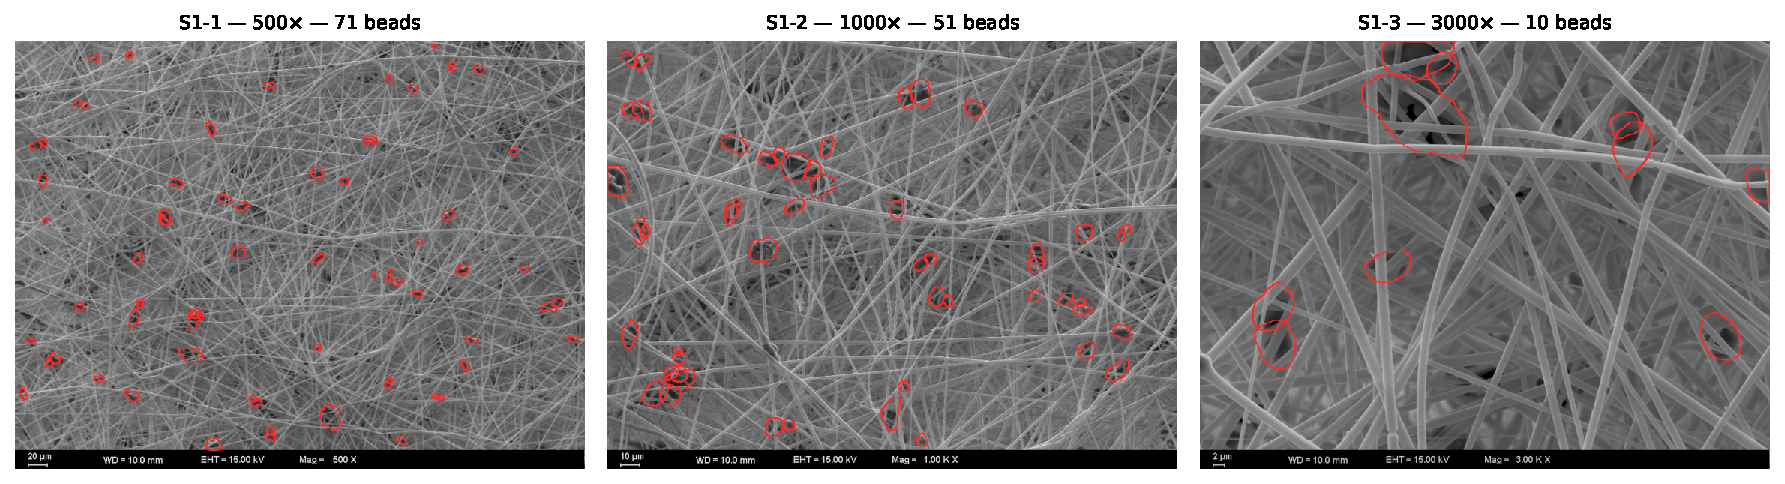
\includegraphics[width=\textwidth]{figures/fig_dataset_overview.pdf}
    \caption{Specimen S1 imaged at $500\times$, $1000\times$ and $3000\times$, with
    the manual bead annotations overlaid in red. The same beads appear at roughly
    14, 29 and 76 pixels across, and the count within the field falls from 71 to 10
    as the field of view narrows.}
    \label{fig:dataset_overview}
\end{figure}

\subsection{Annotation}

The annotations were produced in LabelMe (version 5.4.1) and are supplied as one
JSON file per image. Every annotated object is a closed polygon carrying the
single class label \texttt{bead}, and the polygons contain between 8 and 40
vertices, with a median of 16. Across the 11 images there are 606 annotated
beads. No annotation intersects the instrument banner region described in
Section~\ref{sec:banner}.

The dataset is therefore single-class, as the task is to separate beads from
everything else and no distinction is drawn between bead subtypes.

\subsubsection{What Counts as an Object}
\label{sec:object_definition}

A segmentation result is interpretable only against a definition of the thing
being segmented, so the three rules to which the annotator worked are stated here
rather than left implicit in the polygons. They were specified by the supervisor,
who directs the group that produced the specimens.

The first rule is circularity. The embedded zeolite particles, referred to
throughout this thesis as beads since the two terms denote the same objects, are
approximately circular in projection, so an object is annotated when it presents
as a compact, roughly circular body, and not when it presents as an elongated
fibre segment.

The second is that swellings count. Where a fibre thickens locally into such a
body, that swelling is annotated as a bead even though the fibre passes through
it. In these images this is the common case rather than the exception, which is
why no distinction is drawn between a free bead and a thickened fibre segment.

The third is that a cluster is one object. Where several small beads lie together,
the group is outlined once rather than resolved into its members.

The third rule carries a consequence Chapter~\ref{ch:results} has to live with. A
method that splits a cluster into its visible members is scored as having made a
split error, even where its output may be closer to the number of individual
crystals present. What is counted here is therefore bead sites, and the merge
and split rates of Section~\ref{sec:comparison} measure agreement with that
convention rather than with crystal-level truth; the distinction is revisited
among the limitations in Section~\ref{sec:limitations}.

Two properties of the annotation constrain the implementation and are shown in
Figures~\ref{fig:bead_examples} and \ref{fig:overlap}. The same physical object is
presented at very different resolutions, as the median bead of specimen S4
measures about 8\,$\mu$m at every magnification while spanning 16 pixels at
$500\times$ and 77 at $3000\times$. And beads touch: 8.8\% of annotated bead
pixels lie inside more than one polygon, so the annotation is not a partition of
the image and cannot be stored as one without discarding exactly the regions where
merge and split errors are decided.

\begin{figure}[htbp]
    \centering
    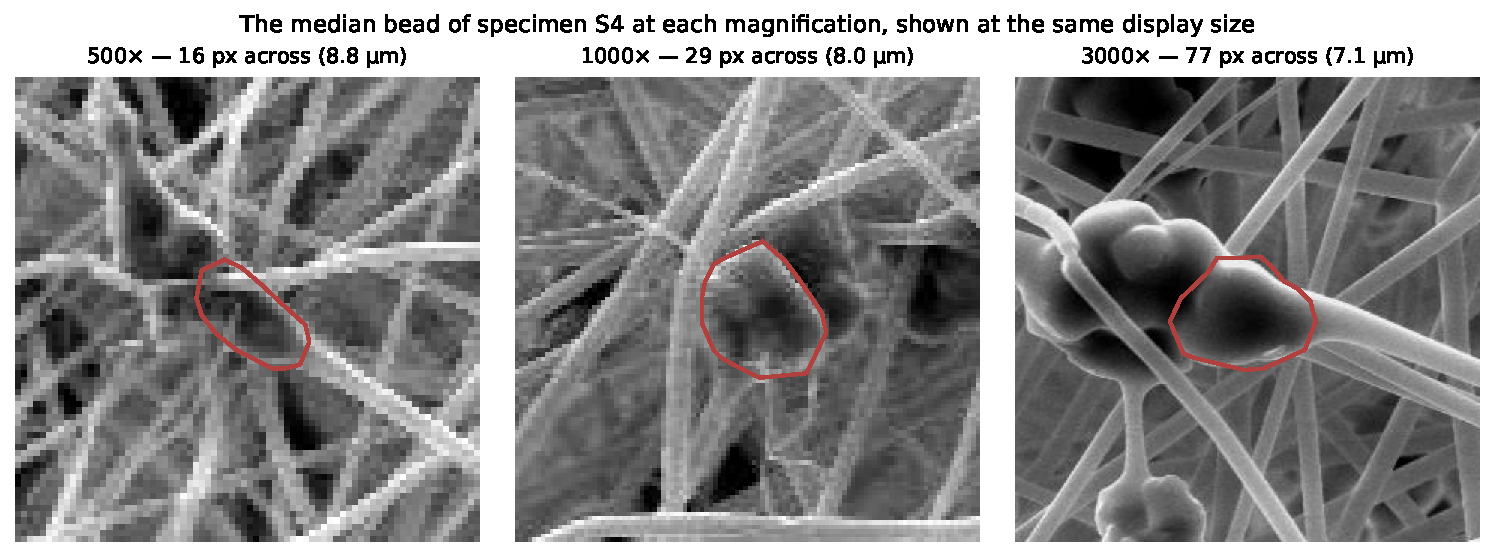
\includegraphics[width=\textwidth]{figures/fig_bead_examples.pdf}
    \caption{The median bead of specimen S4 at each magnification, each crop
    scaled to the same display size. The physical diameter is nearly constant
    while the pixel diameter varies almost fivefold.}
    \label{fig:bead_examples}
\end{figure}

\begin{figure}[htbp]
    \centering
    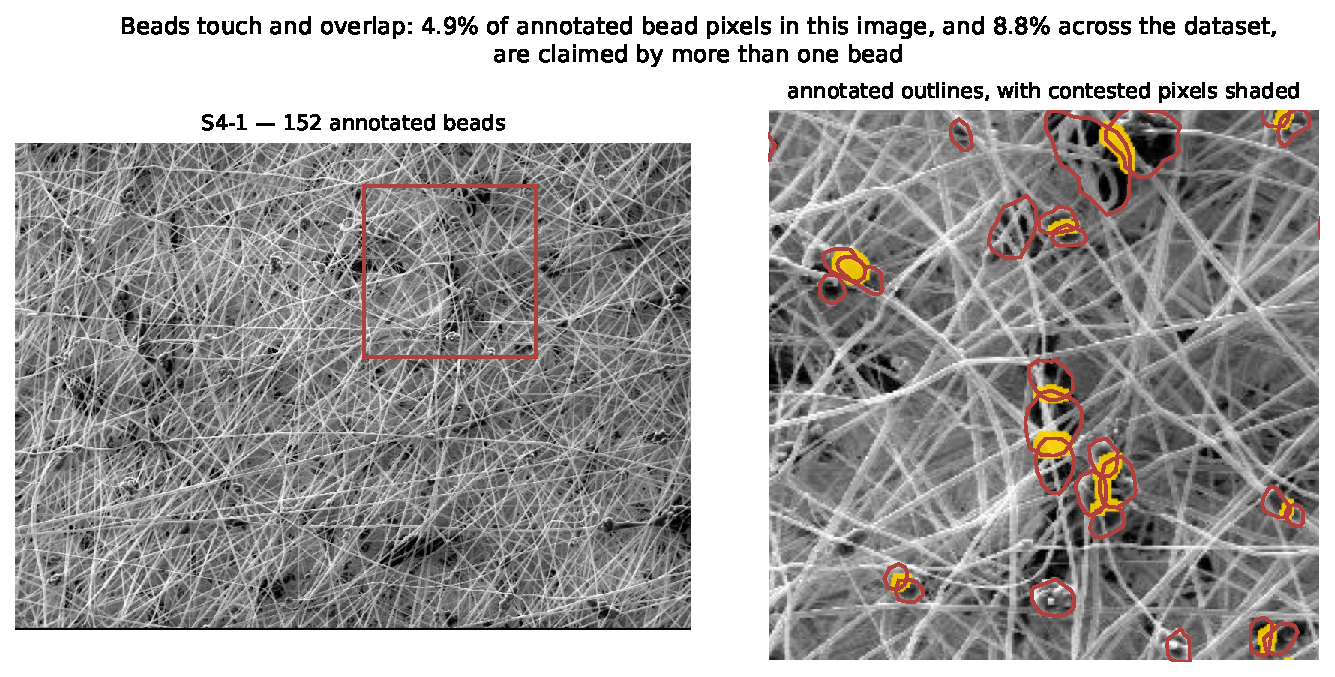
\includegraphics[width=\textwidth]{figures/fig_overlap.pdf}
    \caption{A region of S4-1 in which annotated beads share pixels. Red outlines
    are the manual annotation and shaded pixels are claimed by more than one
    bead.}
    \label{fig:overlap}
\end{figure}

\subsection{Physical Calibration}
\label{sec:calibration}

Each image carries a burned-in scale bar. Measuring the bar in pixels and
dividing by its stated physical length yields the pixel size, and the values
recovered in this way are mutually consistent, since the field width is
$284.4\,\mu$m at $1000\times$ and scales inversely with magnification, as it must.
The resulting calibration is given in Table~\ref{tab:calibration}.

\begin{table}[htbp]
    \centering
    \caption{Pixel size recovered from the burned-in scale bars. The field width is
    inversely proportional to magnification, confirming that the three values form a
    consistent calibration rather than three independent measurements.}
    \label{tab:calibration}
    \begin{tabular}{lrrr}
        \toprule
        Magnification & Field width ($\mu$m) & Pixel size (nm/px) & Beads \\
        \midrule
        $500\times$  & 568.9 & 555.6 & 325 \\
        $1000\times$ & 284.4 & 277.8 & 229 \\
        $3000\times$ & 94.8  & 92.6  & 52  \\
        \bottomrule
    \end{tabular}
\end{table}

Bead size is expressed as an equivalent circular diameter, that is the diameter of
the circle having the same area as the outlined bead. The area is computed
analytically from the polygon vertices $(x_1, y_1), \dots, (x_N, y_N)$ by the
shoelace formula, with indices taken modulo $N$,
%
\begin{equation}
    A = \frac{1}{2}
        \left| \sum_{i=1}^{N} \bigl( x_i \, y_{i+1} - x_{i+1} \, y_i \bigr) \right|,
    \label{eq:shoelace}
\end{equation}
%
rather than by counting the pixels of a rasterised mask. The distinction is not
pedantic in this case, since at $500\times$ the median bead is only about 14 pixels
across, so a one-pixel error along its boundary changes the area by roughly
15\%. The equivalent diameter in micrometres then follows from the pixel size $s$ of
Table~\ref{tab:calibration},
%
\begin{equation}
    d = 2 s \sqrt{\frac{A}{\pi}}.
    \label{eq:equivalent_diameter}
\end{equation}

The calibration can be validated independently of the scale bars. If it is correct,
the physical bead size distribution measured at one magnification should agree with
that measured at another, since all three views image the same specimens. Grouping
every annotated polygon by magnification gives median diameters of 7.92, 7.34 and 6.75\,$\mu$m at $500\times$,
$1000\times$ and $3000\times$ respectively, which is agreement to within 15\%. This
satisfies the criterion set in Section~\ref{sec:objectives} and confirms both the
calibration and the internal consistency of the annotation. The three distributions
are compared in Figure~\ref{fig:bead_statistics}.

\begin{figure}[htbp]
    \centering
    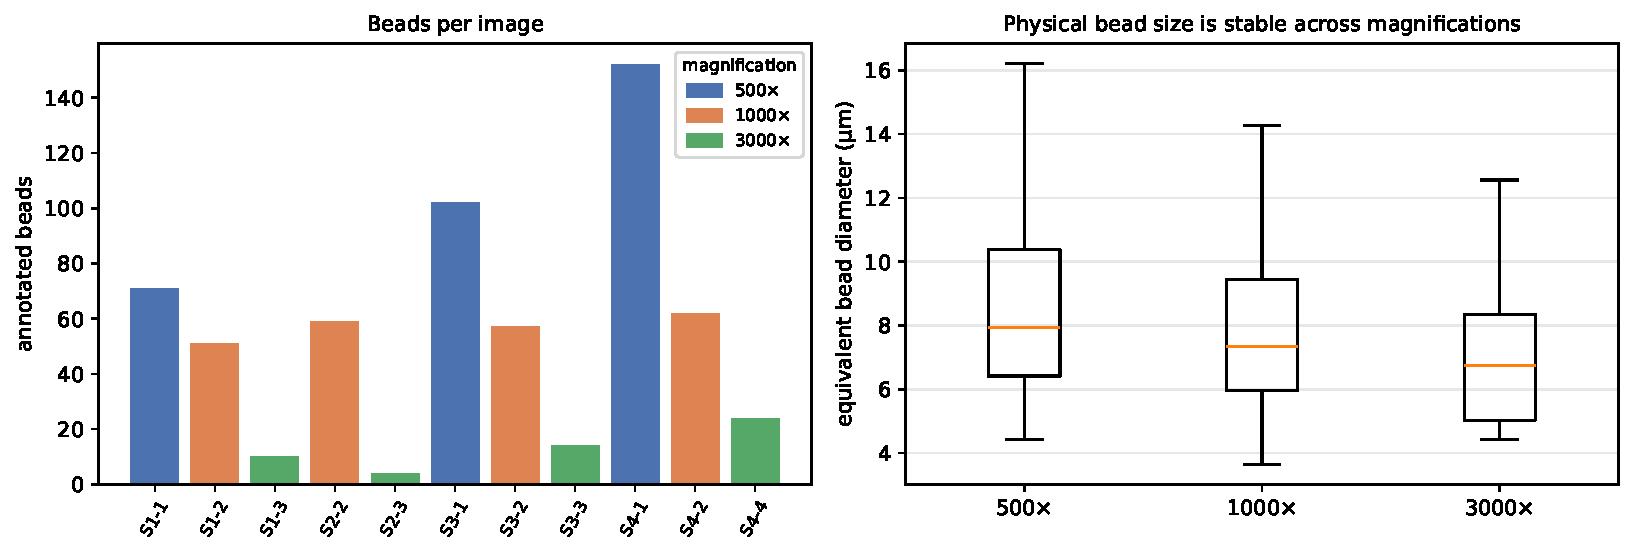
\includegraphics[width=\textwidth]{figures/fig_bead_statistics.pdf}
    \caption{Left: annotated beads per image, coloured by magnification; the
    $3000\times$ images contribute only 52 of the 606 annotated beads. Right:
    equivalent bead diameter in micrometres, grouped by magnification. The three
    distributions overlap, as they must if the calibration is correct.}
    \label{fig:bead_statistics}
\end{figure}

The residual downward trend with magnification, from 7.92 to 6.75\,$\mu$m, is
consistent with a sampling effect rather than a calibration error. At $3000\times$
the field is only 94.8\,$\mu$m wide, so a large bead is more likely to be clipped
by the image border and excluded, and only 52 beads are observed in total.

\subsection{The Instrument Banner}
\label{sec:banner}

Every image carries a burned-in information banner occupying the bottom 32
pixels, containing the scale bar, working distance, accelerating voltage and
magnification. The banner is not part of the specimen: it is high-contrast,
identical in structure across images, and correlates with magnification, so a
network trained on uncropped images could read the magnification off the banner
instead of learning scale-invariant features. It is therefore cropped before any
processing, leaving an effective image size of $1024 \times 736$. No annotation is
lost, since no annotated polygon extends into the banner region, and the
calibration values of Table~\ref{tab:calibration} are extracted once before
cropping and carried forward as metadata.

\subsection{The Supplied Augmentations}
\label{sec:supplied_aug}

The dataset as received contains 143 image--annotation pairs rather than 11. Each
of the 11 originals is accompanied by 12 pre-computed augmented copies: a
horizontal flip, a vertical flip, eight translations of $\pm 150$ pixels along
each axis and in combination, and two horizontal stretches of 20\% and 40\%. The
polygon coordinates were transformed along with the images and remain correctly
registered in every variant.

These copies are nevertheless excluded, for three reasons. The first is
statistical: thirteen copies of one image contain the information of one
image, so reporting 143 images, or 7\,878 bead instances, would misstate the
sample size by a factor of 13.

\begin{figure}[htbp]
    \centering
    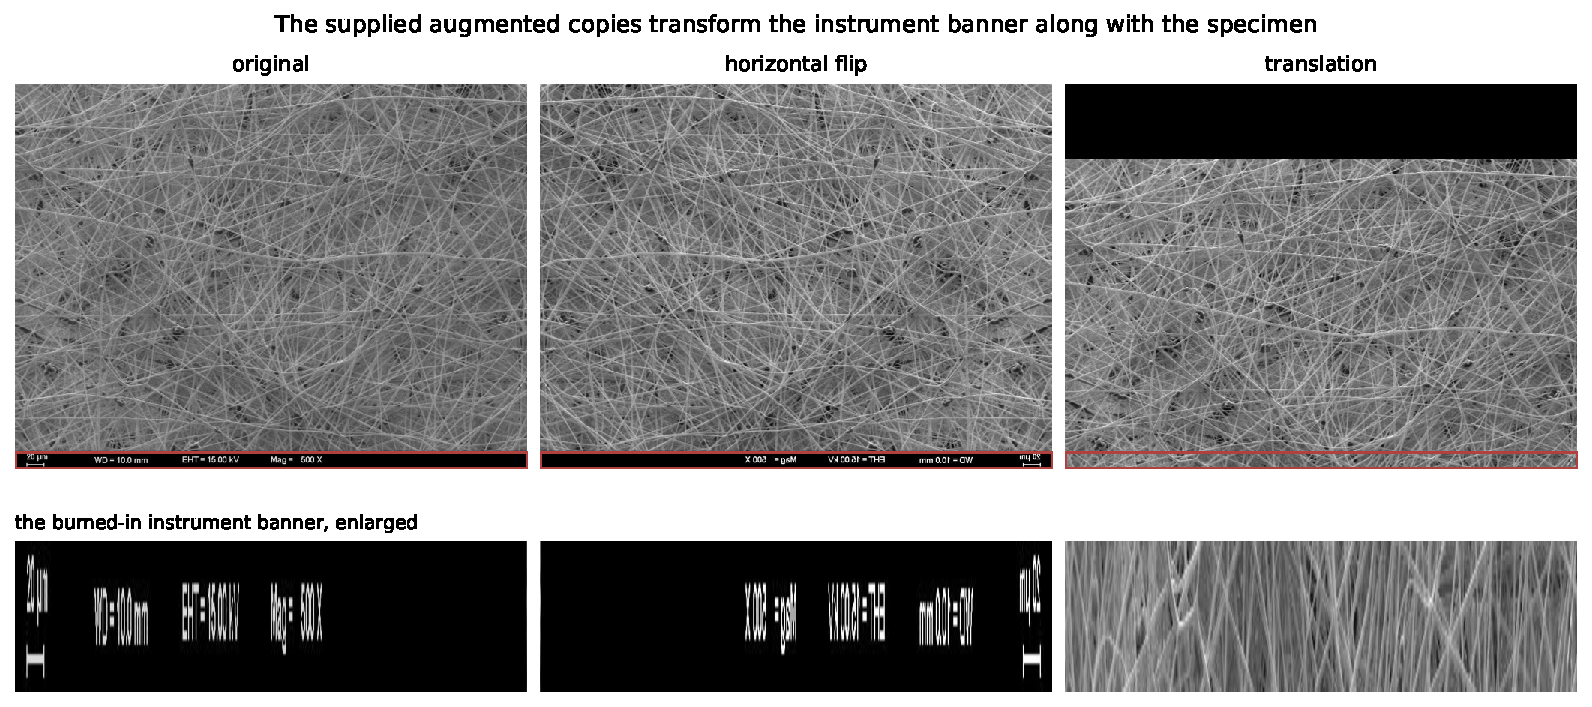
\includegraphics[width=\textwidth]{figures/fig_augmentation_problem.pdf}

    \caption{Three of the 143 supplied files: one original and two of its
    pre-computed augmented copies, with the instrument banner outlined and
    enlarged beneath each. The flip mirrors the burned-in text and the translation
    leaves black fill along the top edge.}
    \label{fig:augmentation_problem}
\end{figure}

The second reason is methodological and more serious. Since the copies were
generated before partitioning, a random split over the 143 files would place
transformed versions of the same source image in both the training and the
test partition, and the test score would then partly measure memorisation.
Augmentation is still used, as it is essential at this sample size, but applied on
the fly during training, after partitioning, so no test image has a transformed
relative in the training set.

The third is visible in Figure~\ref{fig:augmentation_problem}: the transformations
were applied to the whole file, including the instrument banner. The flipped
copies carry mirrored burned-in text and the translated copies carry black fill
along the vacated edge, so the copies are not merely redundant but carry an
artefact a network can key on.

\section{Evaluation Protocol}
\label{sec:protocol}

The four specimens, and not the eleven images, are the independent units of
this dataset. Images S1-1, S1-2 and S1-3 are three views of the same physical
material, sharing its polymer, its spinning parameters and its particular
population of beads, so a partition placing S1-1 in training and S1-3 in testing
measures generalisation to a new magnification of a specimen already seen rather
than to a new specimen.

\begin{figure}[htbp]
    \centering
    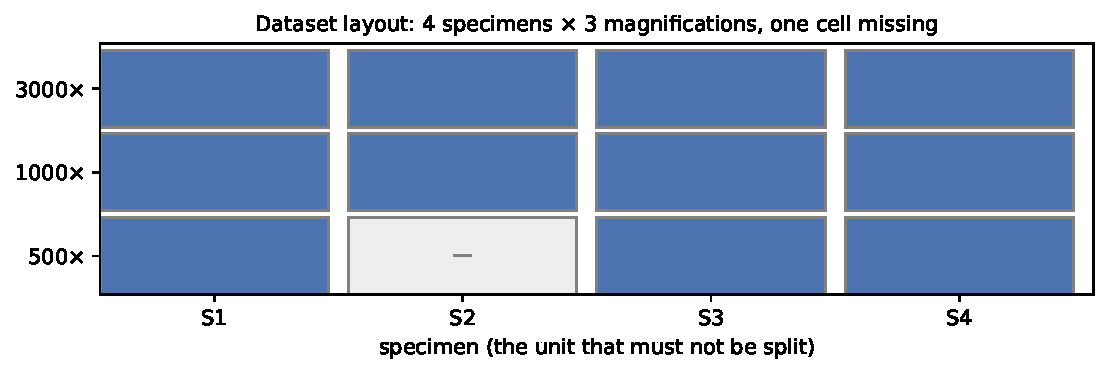
\includegraphics[width=0.75\textwidth]{figures/fig_split_protocol.pdf}
    \caption{Layout of the dataset. Each column is a specimen and each row a
    magnification, and the shaded cells are the 11 available images. Specimen
    S2 has no $500\times$ image.}
    \label{fig:split_protocol}
\end{figure}

The protocol adopted is therefore \emph{leave-one-specimen-out
cross-validation}. Each of the four folds trains on all images of three
specimens and tests on all images of the fourth, so every image is used
for testing exactly once and no specimen is ever split. Results are reported as
the mean over folds together with the spread, which at this sample size is itself
an important number.

To quantify what this protocol costs, and therefore what a naive protocol would
have overstated, a second and deliberately flawed configuration is also run, in
which the 11 images are split at random without regard to specimen. The
difference is reported in Chapter~\ref{ch:results}, and this comparison is one of
the stated contributions of the thesis, since it converts a methodological
argument into a measured quantity.

\section{Methods}

\subsection{Classical Baseline: Otsu Thresholding with Watershed}

The classical pipeline represents current laboratory practice. The cropped
image is contrast-normalised, thresholded with Otsu's method
\cite{otsu1979threshold} and cleaned with morphological opening and closing, and
the resulting binary mask is split into instances by a watershed transform
\cite{vincent1991watersheds} applied to its distance transform with local maxima
as markers. Components smaller than a minimum area, expressed in physical units
through the calibration of Section~\ref{sec:calibration}, are discarded. The
baseline requires no training data, so it is evaluated on all 11 images
directly, with its parameters tuned once on the training folds and held fixed.

\subsection{Semantic Baseline: U-Net}

The semantic baseline is a U-Net \cite{ronneberger2015unet} with a ResNet encoder
\cite{he2016deep} initialised from ImageNet weights \cite{deng2009imagenet},
trained to predict a binary bead-versus-background mask, with instances recovered
afterwards by connected-component labelling. It is included specifically to
isolate the cost of merging: it is expected to segment bead pixels well while
merging clusters of touching beads into single components, and the gap between its
pixel-level and its count-level performance is the quantity of interest.

\subsection{Instance Segmentation: Mask R-CNN}

The primary model is Mask R-CNN \cite{he2017mask} with a ResNet-50 backbone
\cite{he2016deep} and a feature pyramid network \cite{lin2017feature}, initialised
from COCO-pretrained weights \cite{lin2014microsoft}. The region proposal network
proposes candidate boxes, and for each surviving proposal the network predicts a
class, a refined box and a binary mask within the region, so touching beads are
separated by construction. The feature pyramid assigns proposals to levels
according to their size, which is the mechanism by which a single model can handle
beads spanning 14 to 76 pixels across. Anchor scales are set from the empirical
bead size distribution rather than left at their COCO defaults, since the median
bead occupies 0.04\% of the image area.

\subsection{Detection Without Segmentation: Faster R-CNN}

The endpoint this work exists to serve is a count, and a count requires only
detection. Faster R-CNN \cite{ren2015faster} is therefore included as a controlled
ablation of the mask branch of Mask R-CNN: the two share the ResNet-50 and feature
pyramid backbone, the anchor sizes, the cap on detections, the optimiser, the
schedule, the fold definitions and the rule fixing the score threshold on each
fold's training partition. The mask branch is the only difference, so a gap
between them is attributable to it. The same architecture was applied to counting
cells in low-contrast images by Uka et al.\ \cite{uka2020faster}.

Its predictions are stored as boxes with no segmentation field, so it is absent
from every mask-level result: the Aggregated Jaccard Index, Panoptic Quality, the
merge and split rates and the size distribution are mask quantities, and filling
each box to manufacture one would score the method on something it never
predicted. What the ablation can compare is the count, defined identically for
both.

\subsection{One-Stage Alternatives: YOLOv8 and YOLOv5u}

YOLOv8 \cite{redmon2016yolo, jocher2023ultralytics} is the one-stage family of
Section~\ref{sec:onestage}, included to answer a different question from the
ablation above, namely whether a different family of architecture performs better
on this data. It is not a controlled comparison and is not read as one, since it
shares nothing with the region-based models, having a different backbone, an
anchor-free head, a different label assignment rule, a different loss and its own
augmentation and optimiser schedule, so a gap between it and Mask R-CNN identifies
no component as responsible. The segmentation variant is used, so it predicts
masks and is scored on every metric the region-based instance model is.

YOLOv5u is included alongside it, sharing the Ultralytics training loop, the same
three departures from its defaults and the same number of training iterations, while differing
in the backbone and in carrying no mask branch, since the package ships no
segmentation weights for YOLOv5. Two models rather than one make the family
comparison less dependent on a single checkpoint.

The checkpoint is \texttt{yolov5su}, the YOLOv5 backbone fitted by Ultralytics
with the anchor-free, objectness-free split head of YOLOv8, and not the
anchor-based YOLOv5 of the original release. What separates it from
\texttt{yolov8s-seg} is therefore mostly the backbone and the mask branch. The
results are labelled YOLOv5u throughout.

Three settings depart from the package defaults, each for a measured property of
this dataset rather than by search. The input size is held at 1024 rather than the
default 640, since downscaling a $1024 \times 736$ image by 0.625 would take
the median bead at $500\times$ from 14.3 to 8.9 pixels. Mosaic augmentation is
disabled, because composing four images and rescaling roughly halves the apparent
object size while 82.8\% of the beads are already below the small-object
threshold of COCO. Each model is likewise allowed to return up to 400 objects from one
image, since a single image here can hold 152 annotated beads and the default
would discard real detections without reporting that it had.

One consequence has to be stated with the results. The data pipeline of the
package expects a fixed directory of images rather than the crops the region-based
models draw on demand, so both YOLO models train on whole images at 1024
pixels while the region-based models train on $512 \times 512$ crops. Their
training cost is therefore not comparable with that of the region-based models.

\subsection{Preprocessing as an Experimental Factor}
\label{sec:preprocessing_method}

Prior work from this institution reports that the preprocessing applied before a
network sees an image changes materially what it can learn, for images
suffering from non-uniform illumination and low contrast
\cite{uka2020preprocessing}. The present dataset shares the low contrast, with
about eighteen grey levels separating a bead from the surrounding membrane, but
differs in one respect that governs which transforms are worth testing: in
unstained brightfield the background is a smooth field, whereas here it is a dense
fibre network with structure at the same spatial scale as the beads. The
transforms are therefore selected for this material rather than carried across.

Four variants are compared, with the architecture, schedule, fold definitions and
threshold-selection rule held fixed, so any difference is attributable to the
input transform alone:

The first variant applies no transform at all, and it is not merely a formality.
Both detectors are initialised from weights trained on natural images, which carry
expectations about intensity statistics, so a transform can as easily cost
accuracy as buy it, and a variant that loses to this baseline is a finding.

The second is CLAHE, contrast-limited adaptive histogram equalisation, applied
against the narrow separation. It is adaptive rather than global because the
brightness of the membrane varies across a frame by more than the
bead-to-membrane difference.

The third is background subtraction. The beads are darker than the membrane, so
the illumination estimate is a grey closing, which erases dark features while
preserving the slowly varying field. Its footprint has to exceed the largest
object present, and since the largest annotated bead spans 214 pixels the
footprint is set to 257.

The fourth is a median filter, a $3\times3$ median against sensor noise, kept
deliberately small since the median bead is 20 pixels across and a window
approaching that size would remove the object along with the noise.

Each variant is applied to the whole image before cropping, at the single
point where the training and inference paths share code. This is a correctness
requirement rather than a convenience, since a model trained on equalised images
and evaluated on raw ones would still produce numbers, wrong in a way no metric
would reveal.

\section{Evaluation Metrics}

\subsection{Segmentation and Detection Metrics}

Throughout this section, $G = \{g_1, \dots, g_n\}$ denotes the set of annotated bead
masks in an image and $P = \{p_1, \dots, p_m\}$ the set of predicted masks, with
$|\cdot|$ the area of a mask in pixels. The overlap between two masks is measured by
the intersection over union,
%
\begin{equation}
    \mathrm{IoU}(g, p) = \frac{|g \cap p|}{|g \cup p|}.
    \label{eq:iou}
\end{equation}

Detection and mask quality are reported as average precision at an
intersection-over-union threshold of 0.5 ($\mathrm{AP}_{50}$), at 0.75
($\mathrm{AP}_{75}$), and averaged over thresholds from 0.5 to 0.95 following the
COCO protocol \cite{lin2014microsoft}. Average precision at a fixed overlap
threshold originates with the Pascal VOC challenge \cite{everingham2010pascal},
while the COCO variant averages over a range of thresholds so boundary accuracy is
rewarded rather than only detection.

The aggregated Jaccard index \cite{kumar2017dataset} is reported in addition,
since it penalises merges and splits explicitly rather than treating each object
independently. Each annotated bead $g_i$ is assigned the prediction it overlaps
most,
%

\begin{equation}
    j^{*}(i) = \arg\max_{j} \; \mathrm{IoU}(g_i, p_j),
    \label{eq:aji_match}
\end{equation}
%
and writing $M$ for the beads whose best overlap is non-zero, $\bar{M}$ for those
with none, and $U$ for the predictions never selected by any bead,
%
\begin{equation}
    \mathrm{AJI} =
    \frac{\displaystyle\sum_{i \in M} \bigl|g_i \cap p_{j^{*}(i)}\bigr|}
         {\displaystyle\sum_{i \in M} \bigl|g_i \cup p_{j^{*}(i)}\bigr|
          \;+\; \sum_{i \in \bar{M}} |g_i|
          \;+\; \sum_{k \in U} |p_k|}.
    \label{eq:aji}
\end{equation}

%
Every predicted object that matches nothing, and every bead matched by nothing,
therefore enters the denominator and lowers the score, which is what makes the
index sensitive to over-segmentation where a per-object average is not.

Panoptic quality \cite{kirillov2019panoptic} is reported to separate
recognition from delineation. A predicted and an annotated mask are matched when
$\mathrm{IoU}(g, p) > 0.5$, and since no mask can exceed that overlap with more than
one partner, the matching is unique and requires no assignment solver. Writing
$\mathit{TP}$ for the matched pairs and $\mathit{FP}$, $\mathit{FN}$ for the
unmatched predictions and beads,
%
\begin{equation}
    \mathrm{PQ} =
    \underbrace{\frac{\sum_{(g,p) \in \mathit{TP}} \mathrm{IoU}(g,p)}
                     {|\mathit{TP}|}}_{\textstyle \mathrm{SQ}}
    \times
    \underbrace{\frac{|\mathit{TP}|}
                     {|\mathit{TP}| + \tfrac{1}{2}|\mathit{FP}|
                      + \tfrac{1}{2}|\mathit{FN}|}}_{\textstyle \mathrm{RQ}}.
    \label{eq:pq}
\end{equation}

%
The two factors are reported separately as well as combined, since they answer
different questions: segmentation quality $\mathrm{SQ}$ measures how well the
beads that are found are outlined, whereas recognition quality $\mathrm{RQ}$
measures how many were found at all. A method can be strong on one and weak on the
other, and Chapter~\ref{ch:results} shows the distinction matters here.

Finally, one measure deliberately discards instance identity. Flattening each side
to a single binary mask, $\hat{G} = \bigcup_i g_i$ and $\hat{P} = \bigcup_j p_j$,
gives the pixel-level agreement
%

\begin{equation}
    \mathrm{DICE} = \frac{2\,|\hat{G} \cap \hat{P}|}{|\hat{G}| + |\hat{P}|},
    \qquad
    \mathrm{IoU}_{\text{px}} = \frac{|\hat{G} \cap \hat{P}|}
                                    {|\hat{G} \cup \hat{P}|}.
    \label{eq:pixel_dice}
\end{equation}

%
This is the weakest measure in the chapter and is not used to rank anything, since
it cannot distinguish a method that separates two touching beads from one that
fuses them. It is reported for one reason: the semantic segmentation literature,
including the prior work of Section~\ref{sec:epoka_prior}, reports DICE and IoU
computed this way, and those values cannot be read against an average precision,
so computing both from the same predictions is what makes them comparable. The
counts are pooled over images before the ratio is formed, so a frame holding
four beads does not weigh as much as one holding 152.

\subsection{Laboratory Metrics}

Segmentation metrics do not by themselves establish that a method is usable, so
the following are reported as primary outcomes.

The counting error is the error in the number of beads found in an image,
as a fraction of the number actually present, reported both signed and absolute
since a method whose errors cancel behaves differently from one that is biased:
%

\begin{equation}
    e = 100 \times \frac{|G| - |P|}{|G|} \quad (\%),
    \label{eq:counting_error}
\end{equation}
%
positive for an under-count and negative for an over-count, with the sign written
out wherever the quantity appears.

The merge and split rates are the two failure modes that corrupt a
count, and since they have opposite effects on it they are reported separately.
Both are defined through the asymmetric coverage of one mask by another,
%
\begin{equation}
    c_{G}(g, p) = \frac{|g \cap p|}{|g|},
    \qquad
    c_{P}(g, p) = \frac{|g \cap p|}{|p|},
    \label{eq:coverage}
\end{equation}
%
with a threshold of $\tau = 0.5$ throughout. A prediction is a \emph{merge} when it
contains at least half of each of two or more annotated beads, and every bead that
it absorbed counts as merged, whereas an annotated bead is \emph{split} when it
contains at least half of each of two or more predictions:
%
\begin{align}
    \mathrm{merge\ rate} &= \frac{100}{|G|}
        \Bigl|\bigl\{\, g \in G \;:\; \exists\, p \in P,\;
        c_{G}(g,p) \geq \tau \;\wedge\;
        |\{g' \in G : c_{G}(g',p) \geq \tau\}| \geq 2 \,\bigr\}\Bigr|,
    \label{eq:merge_rate} \\[4pt]
    \mathrm{split\ rate} &= \frac{100}{|G|}
        \Bigl|\bigl\{\, g \in G \;:\;
        |\{p \in P : c_{P}(g,p) \geq \tau\}| \geq 2 \,\bigr\}\Bigr|.
    \label{eq:split_rate}
\end{align}

%
Coverage is used rather than intersection over union because the two failures are
asymmetric: a prediction swallowing two beads has a low $\mathrm{IoU}$ with each
while containing both almost entirely, so an overlap-based criterion would miss
exactly the case being measured.

Areal density is beads per square millimetre, the form in which the
measurement is used for process comparison. For an image of $W \times H$
pixels at a pixel size of $s$ micrometres,
%

\begin{equation}
    \rho = \frac{|P| \times 10^{6}}{W H s^{2}}
    \quad (\mathrm{beads\ mm^{-2}}).
    \label{eq:density}
\end{equation}

Size distribution agreement compares the predicted and the manual distributions of
equivalent bead diameter in micrometres, compared by their medians and interquartile
ranges and by a two-sample Kolmogorov--Smirnov test.

\section{Tools and Technologies}

The implementation uses Python with PyTorch. Annotations are parsed from the
LabelMe JSON format and converted to COCO-style instance masks, the classical
baseline uses scikit-image and OpenCV, and figures and statistics are produced
with Matplotlib and NumPy. Full version information is given in
Chapter~\ref{ch:implementation}. No local GPU was available, so the training
stages were run on Google Colab with an NVIDIA T4, with consequences for the
experimental design set out in Section~\ref{sec:environment}.

The dataset comprises 11 SEM images of four electrospun specimens, imaged at
three magnifications and annotated with 606 bead polygons. Each image is
calibrated against its burned-in scale bar, and the calibration is validated by
the agreement of the physical bead size distribution across magnifications. Since
the specimen is the only independent unit, evaluation uses leave-one-specimen-out
cross-validation, and the pre-computed augmented copies supplied with the dataset
are excluded in favour of augmentation applied after partitioning. Six methods,
namely classical thresholding, a semantic U-Net, Mask R-CNN, the same detector
without its mask branch, and the YOLOv8 and YOLOv5u one-stage models, are compared
under this protocol. The next chapter describes how the design is realised in
software.

\chapter{IMPLEMENTATION}
\label{ch:implementation}

\section{Introduction}

This chapter describes the way in which the design of Chapter~\ref{ch:methodology}
is realised in software, that is how the LabelMe annotations are converted into a
trainable format, how the instrument banner and the physical calibration are
handled, how augmentation is applied after partitioning, and how the six methods are
configured and trained.

\section{System Architecture}

The pipeline is organised as five stages, each independently runnable so the
expensive stage, training, does not have to be repeated when only the reporting
changes. Ingest reads the LabelMe JSON files, recovers specimen and
magnification and extracts the pixel calibration from the instrument banner.
Prepare crops the banner, rasterises the polygons into instance masks and emits a
COCO-format annotation file. Partition assigns images to the four
leave-one-specimen-out folds. Train and predict fits each method on each fold's
training partition and predicts on its held-out specimen. Evaluate and report
computes segmentation metrics, counting and merge/split statistics and converts
detections into physical units.

\section{Data Preparation}

\subsection{Annotation Parsing and Rasterisation}
\label{sec:parsing}

Each LabelMe file stores a list of shapes, each carrying a class label, a shape
type and a list of vertices. All 606 shapes are polygons carrying the label
\texttt{bead}, rasterised into per-instance binary masks at full resolution.
Object area is computed analytically from the polygon vertices using the shoelace
formula rather than by counting mask pixels, which avoids a rasterisation bias
significant for the smallest beads, since at $500\times$ the median bead is only
about 14 pixels across, so a one-pixel boundary error changes its area by roughly
15\%. The equivalent circular diameter follows as $d = 2\sqrt{A/\pi}$ and is
converted to micrometres using the magnification-specific pixel size from
Table~\ref{tab:calibration}.

The polygons are kept as polygons rather than flattened into a single label map.
Measurement shows that 8.8\% of all annotated bead pixels are claimed by more than
one polygon, and a label map assigns each pixel to exactly one object, so it would
discard that overlap silently, and precisely in the regions where merge and split
errors are decided. Instance masks are therefore rasterised on demand, one plane
per object.

\subsection{Banner Handling and Calibration}

The instrument banner occupies the bottom 32 rows of every image. Calibration
is performed before cropping, where the scale bar is located as the longest run of
saturated pixels in the lower-left region of the banner and its pixel length divided
by the physical length printed beside it gives the pixel size. The recovered values
are cross-checked by verifying that the field width scales inversely with
magnification, as reported in Section~\ref{sec:calibration}.

The banner rows are then removed, giving a $1024 \times 736$ working image. The
polygon coordinates require no adjustment, since the crop is taken from the bottom
edge and no annotation extends into the banner region.

\subsection{Fold Assignment}

Fold membership is derived from the specimen prefix of the filename, so all
images of one specimen move together. The four folds are S1, S2, S3 and S4. The
assignment is written to disk as an explicit manifest rather than recomputed at
training time, so every method is guaranteed to see identical partitions and
the comparison between them is exact.

The deliberately flawed control configuration described in
Section~\ref{sec:protocol} uses the same machinery with the specimen constraint
disabled, splitting the 11 images at random.

\section{Augmentation}

Augmentation is applied on the fly during training, after partitioning, for the
reasons set out in Section~\ref{sec:supplied_aug}. The pre-computed copies shipped
with the dataset are not used.

The transformations are chosen so as to be label-preserving for this modality.
Images of a non-woven membrane have no canonical orientation, so horizontal and
vertical flips and rotations in multiples of $90^{\circ}$ are physically meaningful.
Random scaling is included deliberately and with a wider range than would be usual,
since scale robustness across the $500\times$ to $3000\times$ span is the central
difficulty of the dataset. Brightness and contrast jitter model the variation in
detector gain between sessions. Elastic and shear deformations are excluded, as they
would distort bead shape, and bead shape is a measured output rather than an
incidental property.

Random cropping to fixed-size tiles is used both as augmentation and as a practical
measure, since a $1024 \times 736$ image containing up to 152 small beads is
awkward to fit in memory at the batch sizes needed for stable training.

\section{Model Configuration}

\subsection{Mask R-CNN}

The primary model uses a ResNet-50 backbone with a feature pyramid network,
initialised from COCO-pretrained weights. Two departures from the defaults are
required by the data.

The anchor sizes are set from the empirical bead size distribution rather than left
at their COCO values. The median bead occupies 0.04\% of the image area, which is
far smaller than a typical COCO object, and default anchors would leave the smallest
beads without a well-matched proposal.

The maximum number of detections per image is raised well above the COCO default of
100, since a single $500\times$ image contains up to 152 beads and the default
would silently truncate the count, which is an error that would corrupt precisely
the quantity being measured.

\subsection{U-Net Baseline}

The semantic baseline uses a ResNet encoder initialised from ImageNet weights
together with a symmetric decoder with skip connections. It is trained with a
combined cross-entropy and Dice loss to counter the strong
foreground/background imbalance, since bead pixels constitute only 2 to 20\% of a
image. Writing $\hat{y}_i$ for the predicted probability at pixel $i$ and
$y_i \in \{0,1\}$ for the annotation,
%
\begin{equation}
    \mathcal{L} =
    \underbrace{-\frac{1}{N}\sum_{i=1}^{N}
      \bigl[\, y_i \log \hat{y}_i + (1 - y_i) \log (1 - \hat{y}_i) \,\bigr]}
      _{\textstyle \text{cross-entropy}}
    \;+\;
    \underbrace{1 - \frac{2 \sum_i \hat{y}_i y_i + \varepsilon}
                        {\sum_i \hat{y}_i + \sum_i y_i + \varepsilon}}
      _{\textstyle \text{Dice}},
    \label{eq:dice_bce}
\end{equation}
%
with $\varepsilon = 1$ guarding the degenerate case of an empty crop.
Cross-entropy alone is minimised well by a nearly empty prediction when the
foreground is this sparse, whereas the Dice term is scale-invariant in the number of
foreground pixels and supplies the gradient that prevents this.

The instances are recovered from the predicted mask by connected-component
labelling, with no boundary-aware post-processing. The omission is deliberate, since
connected components cannot separate two beads whose predicted regions touch, and
adding a boundary-aware correction would hide that limitation rather than measure
it. Whether it costs anything on this data is reported as the merge rate in
Chapter~\ref{ch:results}.

\subsection{Faster R-CNN}

Faster R-CNN is built from the same torchvision family as Mask R-CNN and from the
same COCO-pretrained ResNet-50 and feature pyramid weights, with the mask predictor
absent. The anchor ladder, the cap of 400 detections per image, the region proposal limits,
the optimiser, the learning-rate schedule and the input-size pinning are set by the
same code path, so the two models differ in the mask branch and in nothing else
that was configured.

The consequence for the output format is deliberate. The predictions are written as
boxes with no segmentation field, and the evaluation module therefore leaves every
mask-level metric unset for this method rather than filling each box with a
rectangle to score it. ``Did not segment'' and ``segmented badly'' are
different claims, and a zero would report the second while meaning the first.

\subsection{YOLOv8 and YOLOv5u}

YOLOv8 is trained through the Ultralytics package rather than through the
torchvision path, which imposes two implementation differences on which the
results depend.

The package expects a dataset on disk in its own layout, so each fold is exported
to a scratch directory as images plus one label file per image, with the instance
polygons converted to normalised vertex lists. That export is written to local
disk rather than to the mounted Drive, since the iteration count converts to roughly
750 epochs over eight images and the package rewrites its \texttt{last.pt}
checkpoint at the end of every epoch, which over a network filesystem would
dominate the run time.

The package also drives its own training loop, so the schedule, the augmentation
and the optimiser are its defaults rather than those in
Table~\ref{tab:training_config}, with three exceptions set explicitly: the input
size at 1024, mosaic augmentation disabled and the detection cap at 400. Its
predictions are converted to the same run-length-encoded mask format every other
mask-predicting method writes.

Both YOLO families are handled by one script, which selects the family from the
weights filename and writes each to its own prediction file. Both are reported in
Chapter~\ref{ch:results}, although not on the same footing, since the package
ships no segmentation variant of YOLOv5 and that family therefore enters on the
box-only path alongside Faster R-CNN.

One point of nomenclature has to be stated, since the version numbers invite a
reading the weights do not support. The checkpoint used is \texttt{yolov5su.pt},
which is not the YOLOv5 of the original release: Ultralytics distributes the
YOLOv5 backbone fitted with the anchor-free, objectness-free split head of YOLOv8.
Comparing it against \texttt{yolov8s-seg} therefore varies mostly the backbone and
the presence of a mask branch, and is not the anchor-based against anchor-free
comparison the version numbers suggest. The results are labelled YOLOv5u
throughout.

\subsection{Classical Baseline}

The classical pipeline is implemented with scikit-image, comprising CLAHE contrast
normalisation, Otsu thresholding, morphological opening and closing, the distance
transform, local-maximum markers and watershed. Its three free parameters, namely
the morphological kernel size, the minimum accepted object area in $\mu$m$^2$ and
the marker suppression distance, are tuned by grid search on the training partition
of each fold and are then held fixed for that fold's test specimen, so it is
subject to the same protocol as the learned methods.

\section{Training Setup}

Each of the four folds is trained independently from the same initialisation, and no
fold's held-out specimen influences any choice made during its training, neither the
number of iterations nor the score threshold applied to the output. The threshold is
selected separately for each fold by maximising $F_1$ on that fold's own training
partition.

The configuration is reported in Chapter~\ref{ch:results},
Table~\ref{tab:training_config}, rather than here, because the values that matter
are the ones that the runs actually used. Stating a planned configuration in this
chapter and a measured one in the next invites the two to drift apart, and it is the
measured one against which the results have to be read.

\section{Development Environment}
\label{sec:environment}

Development is in Python with PyTorch \cite{paszke2019pytorch} and torchvision.
Annotation handling and figures use NumPy, Pillow and Matplotlib, the classical
baseline uses scikit-image \cite{vanderwalt2014scikit} and SciPy, and average
precision is computed with the reference COCO implementation
\cite{lin2014microsoft}.

No local GPU was available, so the training stages run on Google Colab with an
NVIDIA T4. This constrains the design in two ways. A session can be interrupted,
so each stage writes its predictions to persistent storage and can be resumed
independently rather than the pipeline being one long run. And the total GPU time
is limited, which is why the comparison is between six methods under one protocol
rather than a wider hyperparameter search, since the leave-one-specimen-out
protocol already multiplies every configuration by four.

The iteration counts and every other setting the runs actually used are recorded
in Table~\ref{tab:training_config}, which \texttt{make\_tables.py} writes from the
metadata each training script stores alongside its predictions. Wall-clock cost is
instrumented separately by \texttt{runtime.py} and reported in
Table~\ref{tab:runtime}.

\section{Challenges and Solutions}
\label{sec:challenges}

Six problems were encountered while building the pipeline, and each changed a
design decision.

The augmented copies could not be used as supplied. The dataset arrives
as 143 image--annotation pairs, which initially appears to be a usable sample
size, while the filenames reveal 11 originals with 12 transformed copies each.
The transformations are correctly applied, so the copies are not defective, but
they are not independent either, and letting them cross a partition boundary would
have produced optimistic results.

The banner is augmented along with the image. The flipped copies show the
instrument banner mirrored and the translated copies carry black padding along the
vacated edge, which reinforced the decision to crop it before any processing.

Object size varies sixfold across the dataset. The median bead is 14
pixels across at $500\times$ and 76 at $3000\times$, which drove the choice of a
feature pyramid backbone, the resetting of the anchor scales and the wide
random-scaling range in the augmentation policy.

Augmentation initially shifted every mask by one pixel. Reflections were
first implemented as $x \mapsto W - 1 - x$, correct for an integer pixel index but
not for polygon vertices, which are continuous coordinates and reflect as
$x \mapsto W - x$. Half a pixel at each edge is invisible on a large object, but
the mean bead here is 17 pixels across, so a one-pixel boundary shift moves
roughly 13\% of its area on every flipped training sample. The fault was found by
rasterising the transformed polygons and comparing them against the directly
transformed raster mask, which agree to an intersection over union of 0.9995 under
the correct convention and 0.87 under the incorrect one. That check is now
permanent in the test suite, since the failure produced no error message and no
visibly wrong image, only slightly wrong labels.

Evaluating a thousand objects per image was forty times slower than
necessary. Instances were initially held as full-frame masks, one
$1024 \times 736$ array per object, and the classical baseline emits over a
thousand objects for a single image, so its parameter search spent almost all
its time reading zeros: a single Aggregated Jaccard Index computation took 5.95
seconds. Holding each instance as a bounding box plus a mask covering only that
box, and computing intersections only for pairs whose boxes overlap, reduced that
to 0.02 seconds and the full parameter search from over an hour to a few minutes.

The smoke run destroyed a completed set of results. The fast correctness
check of Section~\ref{sec:deployment} originally wrote its predictions to the same
directory as a real run, so re-running it after a completed four-fold experiment
silently overwrote several hours of predictions with output from eight training
iterations. A smoke run produces a well-formed predictions file, so nothing fails
and nothing warns, and the only symptom is that every subsequently reported number
is wrong. The fix is structural rather than procedural: a smoke run now redirects
its working and results directories before any pipeline module is imported.

\section{Code Organization}

Table~\ref{tab:modules} lists the modules and what each is responsible for.

\begin{table}[htbp]
    \centering
    \caption{The modules of the implementation. Each concern is owned by one
    file, so a rule such as the partitioning guarantee is written once and
    inherited everywhere it applies.}
    \label{tab:modules}
    \begin{tabular}{p{0.32\textwidth}p{0.58\textwidth}}
        \toprule
        Module & Responsibility \\
        \midrule
        \texttt{config.py} & Dataset facts, calibration constants and paths, in one place so no constant is defined twice. \\
        \texttt{dataset\_stats.py} & Descriptive statistics and the dataset figures of Chapter~\ref{ch:methodology}. \\
        \texttt{prepare\_data.py} & Banner cropping and COCO conversion. \\
        \texttt{folds.py} & The fold manifests for both protocols. \\
        \texttt{data\_io.py} & Annotation loading, polygon rasterisation and the augmentation geometry, free of any deep-learning dependency so the classical baseline and the evaluation code run without PyTorch. \\
        \texttt{datasets.py}, \texttt{models.py} & The PyTorch dataset, the Mask R-CNN configuration and the U-Net definition. \\
        \texttt{train\_maskrcnn.py}, \texttt{train\_fasterrcnn.py}, \texttt{train\_unet.py}, \texttt{train\_yolo.py}, \texttt{classical.py} & The six methods, the two one-stage models being driven by a single script that selects the family from the weights filename. \\
        \texttt{predio.py} & The shared prediction format. Every method writes COCO results, the mask-predicting ones as run-length-encoded masks and the box-only ones as boxes with no segmentation field. \\
        \texttt{metrics.py}, \texttt{evaluate.py} & Segmentation metrics, counting and merge/split statistics, and physical quantification. \\
        \texttt{runtime.py} & The wall-clock instrumentation behind Table~\ref{tab:runtime}. \\
        \texttt{make\_tables.py}, \texttt{make\_figures.py} & The tables and figures of Chapter~\ref{ch:results} and the dataset figures, generated from the measured metrics. \\
        \texttt{run\_all.py} & Runs the pipeline end to end, with a \texttt{-{}-smoke} mode that executes a few iterations to verify nothing crashes before committing hours of GPU time. \\
        \texttt{notebooks/Thesis\_Colab.ipynb} & The notebook used to run the training stages. \\
        \bottomrule
    \end{tabular}
\end{table}

Chapter~\ref{ch:results} is populated by \texttt{make\_tables.py} rather than by
hand, so no number can reach the thesis without a run having produced it.

\section{Deployment}
\label{sec:deployment}

The pipeline is deployed as a Google Colab notebook that clones the repository,
mounts the specimen data from Drive and runs each stage as a separate cell. Three
properties of that arrangement are deliberate.

Each stage is independently resumable. A Colab session can be
disconnected at any point, and a four-fold run of six methods takes long enough
that this is likely rather than merely possible, so every stage writes its
predictions to persistent storage before the next begins.

A smoke path runs the entire pipeline in about two minutes. It executes
eight training iterations per fold and a single classical parameter combination.
Its numbers are meaningless; its purpose is to establish that nothing crashes
before committing hours of GPU time. It writes to a separate working directory,
for the reason given in Section~\ref{sec:challenges}.

Reporting is reproducible from stored metrics. The evaluation and
table-generation stages read only the saved predictions, so the tables and figures
of Chapter~\ref{ch:results} regenerate without repeating any training, and a
change in how a result is presented cannot alter the result.

The complete repository, including the notebook, is available at
\url{https://github.com/ErlindSkura/Erlind_Skura_Thesis}.

The pipeline separates ingest, preparation, partitioning, training and evaluation
so the partitioning guarantee of Chapter~\ref{ch:methodology} is enforced in one
place and inherited by every method. The two decisions that most affect the
validity of the results, discarding the pre-computed augmentations and cropping
the instrument banner, both follow from properties of the data discovered during
preparation rather than from convention. The next chapter reports what the
pipeline produces.

\chapter{RESULTS AND DISCUSSION}
\label{ch:results}

% =====================================================================
% Every table in this chapter is generated by code/make_tables.py from
% results/metrics.json, which is written by the training and evaluation
% scripts. No cell is typed by hand. Re-running the pipeline updates the
% numbers; it cannot leave the chapter silently contradicting them.
%
% The section structure follows the objectives set out in Section 1.4, so
% that each result answers a stated question.
% =====================================================================

\section{Introduction}

This chapter reports the experimental results. It establishes the dataset
characterisation and calibration, reports the six segmentation methods under the
leave-one-specimen-out protocol of Section~\ref{sec:protocol} together with two
ablations of the input, tests the protocol against its naive alternative,
separates training from test accuracy, and reports the physical quantities the
laboratory uses: bead count, areal density and the size distribution in
micrometres.

Three results are negative and each is reported as prominently as the positive
ones. Mask R-CNN does not reach the accuracy criterion of
Section~\ref{sec:objectives}. The naive partitioning protocol does not overstate
performance in the way the literature on small microscopy datasets would lead one
to expect. And none of the three preprocessing transforms improves detection,
although one measurably improves counting.

\section{Dataset Characterisation}

The descriptive analysis is reported in Chapter~\ref{ch:methodology}: 606
annotated beads across 11 micrographs of four specimens at three magnifications,
with the pixel calibration of Table~\ref{tab:calibration}.

The first objective of Section~\ref{sec:objectives} is met. The median equivalent
bead diameter is 7.92\,$\mu$m at $500\times$, 7.34\,$\mu$m at $1000\times$ and
6.75\,$\mu$m at $3000\times$, an agreement of within 15\% against a stated
criterion of 20\%. Since the three magnifications image the same four specimens,
this is evidence both that the calibration is correct and that the annotation is
internally consistent across magnifications, as an annotator who had applied a
different size threshold at different magnifications would have broken it.

The residual downward trend is consistent with border clipping rather than with
calibration error. At $3000\times$ the field is 94.8\,$\mu$m wide, so a bead of
8\,$\mu$m occupies a much larger fraction of it and is correspondingly more likely
to intersect the image boundary and be excluded. Only 52 of the 606 beads come
from $3000\times$ micrographs, so this group is also the noisiest.

\section{Experimental Setup}

\subsection{Training Configuration}

Table~\ref{tab:training_config} records the configuration used. Both models were
trained independently on each of the four folds from the same initialisation, on a
single NVIDIA T4.

% Generated by code/make_tables.py from results/metrics.json.
% Do not edit by hand: re-run the pipeline instead.
\begin{table}[htbp]
    \centering
    \caption{Training configuration actually used. Both models were trained
    independently on each of the four folds from the same initialisation.}
    \label{tab:training_config}
    \begin{tabular}{lll}
        \toprule
        Setting & Mask R-CNN & U-Net \\
        \midrule
        Backbone        & ResNet-50 + FPN   & ResNet-34 encoder \\
        Initialisation  & COCO              & ImageNet \\
        Optimiser       & SGD, momentum 0.9 & Adam \cite{kingma2015adam} \\
        Learning rate   & 0.005 (cosine)  & 0.0003 (cosine) \\
        Batch size      & 4        & 8 \\
        Iterations      & 1500        & 1500 \\
        Crop size       & $512 \times 512$  & $512 \times 512$ \\
        Loss            & RPN + box + mask  & Cross-entropy + Dice \\
        \bottomrule
    \end{tabular}
\end{table}


\subsection{Justification of Training Hyperparameters}
\label{sec:training_config}

Four settings depart from what a default configuration would give, and each was
chosen from a measured property of the data rather than by search. No
hyperparameter was tuned against performance, so none can have been fitted to the
test partitions.

\textbf{Anchor sizes: 8, 16, 32, 64 and 128 pixels.} The torchvision default
begins at 32 pixels, whereas the median bead is 14 pixels across at $500\times$,
so under the default most objects at the lowest magnification would have no anchor
within a factor of two of their size. The chosen ladder brackets the observed
range of 14 to 76 pixels, widened at both ends to cover the random scaling applied
during training.

\textbf{Detection cap: 400 per image.} The COCO default is 100, while micrograph
Z6-1 contains 152 annotated beads, so the default would have truncated its output
silently and biased exactly the quantity this work measures. The cap never binds
for the region-based detectors, and Section~\ref{sec:yolo_results} reports the one
method for which it does.

\textbf{Crop size $512 \times 512$ with scale jitter from 0.5 to 2.0.} A
leave-one-specimen-out training partition holds eight micrographs, so training on
whole images would present eight distinct inputs, whereas random crops draw a
different field of view each time. The scaling range is wider than usual because
robustness across a sixfold range in apparent object size is the central
difficulty of this dataset.

\textbf{Score threshold: selected per fold on training data.} The threshold
applied to each detector was chosen by maximising $F_1$ at an intersection over
union of 0.5 on the \emph{training} partition of each fold. For Mask R-CNN the
selected values were 0.65, 0.65, 0.70 and 0.60 on folds Z2, Z4, Z5 and Z6, for
Faster R-CNN 0.60, 0.60, 0.65 and 0.65, for YOLOv8 0.15, 0.30, 0.15 and 0.15, and
for YOLOv5u 0.20, 0.35, 0.20 and 0.10. This is the one free parameter of each
learned pipeline, and selecting it on test data would have inflated every number
in this chapter. The U-Net thresholds and the three parameters of the classical
pipeline were chosen the same way.

The gap between the two families is itself a finding. The region-based detectors
settle between 0.60 and 0.70 whereas the two YOLO models maximise training $F_1$
between 0.10 and 0.35, so the same criterion selects an operating point three to
four times lower. This is a statement about how the families calibrate their
confidence scores rather than about their accuracy, and it makes raw detection
counts incomparable across them. Both YOLO models also select their lowest
threshold on the fold holding out Z6, which is the fold on which both over-count
most severely, and Section~\ref{sec:yolov5_results} takes that coincidence apart.

The number of training iterations, 1500, was set by the available GPU budget
rather than by a convergence criterion, and is recorded as a limitation in
Section~\ref{sec:limitations}.

\subsection{Computational Cost}
\label{sec:runtime}

Every method was trained on a single NVIDIA T4 through Google Colab. Four
quantities are recorded per method: the median time per optimiser step, the steps
in an epoch, the time per epoch and the wall-clock time for one fold. Training
draws random $512 \times 512$ crops on demand rather than iterating a fixed set,
so there is no natural epoch boundary; an epoch is defined here as one
crop-equivalent pass over the eight training micrographs of a fold, which at this
crop size is 2.875 crops per micrograph. Step times are medians, measured with the
device synchronised before the clock is read, and exclude the first step of each
fold, which carries one-off allocation and kernel selection.

% Emitted by make_tables.py only once at least one method has recorded timings.
% The sentence that cites the table lives inside the conditional as well, so that
% this file compiles with no undefined reference before the instrumented runs
% exist.
\IfFileExists{results/table_runtime.tex}{%
    Table~\ref{tab:runtime} gives these figures for every method.
    % Generated by code/make_tables.py from results/metrics.json.
% Do not edit by hand: re-run the pipeline instead.
\begin{table}[htbp]
    \centering
    \caption{Training cost per fold, averaged over the four leave-one-specimen-out
    folds. Trained on Tesla T4. An epoch is one crop-equivalent pass over the fold's eight training
    images. Step times are medians, measured with the device synchronised,
    and exclude the first step.}
    \label{tab:runtime}
    \begin{tabular}{lrrrrrr}
        \toprule
        Method & Batch & s/step & Steps/epoch & s/epoch & Epochs & Total (min) \\
        \midrule
        U-Net + CC       & 8 & 0.488 & 2.9 & 1.7 & 507.2 & 14.5 \\
        Mask R-CNN       & 4 & 0.396 & 5.8 & 2.4 & 253.5 & 10.3 \\
        Faster R-CNN     & 4 & 0.339 & 5.8 & 2.1 & 253.5 & 8.9 \\
        YOLOv8           & 4 & 1.280 & 2.0 & 2.6 & 729.2 & 32.0 \\
        YOLOv5u          & 4 & 1.183 & 2.0 & 2.4 & 729.2 & 29.6 \\
        \bottomrule
    \end{tabular}
\end{table}
%
}{}

Three comparisons in that table bear on conclusions drawn later in this chapter.

\textbf{The mask branch is nearly free.} Mask R-CNN costs 10.3 minutes per fold
against 8.9 for Faster R-CNN, a 15\% premium for the branch that produces the
per-instance masks. Every mask-level quantity reported in this work is bought with
that 15\%.

\textbf{Both YOLO models cost about three times as much as Mask R-CNN.} At 32.0
minutes per fold for YOLOv8 and 29.6 for YOLOv5u against 10.3, and at 1.280 and
1.183 seconds per step against 0.396 at the same batch size, they are the two most
expensive methods measured. The difference is input size rather than architecture,
since their data pipeline expects a fixed image directory rather than crops drawn
on demand, so both trained on whole $1024$-pixel micrographs while the others
trained on $512 \times 512$ crops.

\textbf{The campaign as a whole is small.} Summed over every run reported in this
chapter, six methods, three preprocessing variants, the threefold-magnified run
and the random-split control, four folds each, training consumed 10.8 hours of T4
time. That matters for reproducibility rather than performance: the complete set
of results regenerates within a day on freely available hardware.

\subsection{Evaluation Protocol}

Every micrograph is scored exactly once, by the model of the fold that held its
specimen out, so the eleven per-image results are mutually independent and pooling
them gives a single estimate over the whole dataset.

All six methods are evaluated by the same code, on the same prediction format and
against the same ground truth, since a controlled comparison is meaningful only if
the differences between methods come from the methods. The two exceptions are
declared rather than absorbed: Faster R-CNN and YOLOv5u predict boxes and no
masks, so their average precision is computed at box overlap and they are absent
from every mask-level column, which is a different statement from scoring zero on
it. Metrics are reported at the three levels defined in
Section~\ref{sec:protocol}, because a single number conceals the failure modes
that matter here: a method can score acceptably on average precision and fail
completely on the count, as Section~\ref{sec:counting} shows.

\subsection{Fold Composition}

% Generated by code/make_tables.py from results/metrics.json.
% Do not edit by hand: re-run the pipeline instead.
\begin{table}[htbp]
    \centering
    \caption{Leave-one-specimen-out fold composition and the bead counts
    Mask R-CNN produced for each held-out specimen. Counting error is signed,
    positive meaning an over-count, and is the mean over the fold's micrographs
    rather than the difference between the two count columns.}
    \label{tab:folds}
    \begin{tabular}{llrrrr}
        \toprule
        Fold & Test specimen & Micrographs & Annotated & Predicted & Counting error (\%) \\
        \midrule
        1 & Z2 & 3 & 132 & 110 & -21.9 \\
        2 & Z4 & 2 & 63 & 43 & -40.3 \\
        3 & Z5 & 3 & 173 & 90 & -27.1 \\
        4 & Z6 & 3 & 238 & 319 & 64.7 \\
        \midrule
        \multicolumn{2}{l}{\textbf{Total}} & \textbf{11} & \textbf{606} & \textbf{562} & \\
        \bottomrule
    \end{tabular}
\end{table}


The folds are markedly unbalanced, as specimen Z4 contributes only 63 beads across
two micrographs while Z6 contributes 238 across three. Per-fold results are
therefore reported individually as well as averaged, since a mean over four folds
of this size is not a stable summary on its own.

One feature of that table appears to be an error and is not. Fold Z6 shows 238
annotated beads against 319 predicted, an over-count of 34.0\% on the totals, next
to a counting error of $-64.7\%$. The count columns are fold totals, whereas the
error column is the mean over the fold's three micrographs of the per-micrograph
signed error, and on Z6 those are $+8.6\%$, $-119.4\%$ and $-83.3\%$. The two
large over-counts fall on the sparsely populated micrographs and the near-miss on
the densest, so the unweighted mean is nearly twice the ratio of the totals. The
per-micrograph figure is the one reported throughout, since the laboratory
measures one micrograph at a time.

\section{Segmentation Results}

\subsection{Mask R-CNN}

% Generated by code/make_tables.py from results/metrics.json.
% Do not edit by hand: re-run the pipeline instead.
\begin{table}[htbp]
    \centering
    \caption{Mask R-CNN under leave-one-specimen-out cross-validation.}
    \label{tab:maskrcnn_results}
    \begin{tabular}{lrrrr}
        \toprule
        Test specimen & $\mathrm{AP}_{50}$ & $\mathrm{AP}_{75}$ & AP & AJI \\
        \midrule
        Z2 & 0.334 & 0.079 & 0.125 & 0.305 \\
        Z4 & 0.355 & 0.129 & 0.155 & 0.397 \\
        Z5 & 0.223 & 0.043 & 0.100 & 0.273 \\
        Z6 & 0.281 & 0.083 & 0.101 & 0.323 \\
        \midrule
        Mean $\pm$ s.d. & 0.298 $\pm$ 0.059 & 0.084 $\pm$ 0.035 & 0.120 $\pm$ 0.026 & 0.325 $\pm$ 0.053 \\
        \bottomrule
    \end{tabular}
\end{table}


Mask R-CNN reaches $\mathrm{AP}_{50} = 0.298 \pm 0.059$ averaged over the four
folds, with an Aggregated Jaccard Index of $0.325 \pm 0.053$ and a Panoptic
Quality of 0.351.

\textbf{This meets neither criterion of Section~\ref{sec:objectives}, although it
falls two thousandths short of the second.} Against the
$\mathrm{AP}_{50} \geq 0.70$ recorded at the proposal stage the shortfall is not
close. Against the literature-anchored 0.30, which is what a standard Faster R-CNN
reaches on a benchmark whose objects are within two pixels of the median size here
\cite{xu2022tiny}, the result is 0.298 and is reported as not met, since rounding
it up would buy a claim worth less than the admission.

The decomposition of Panoptic Quality is more informative than the headline
figure. Segmentation Quality, the mean intersection over union of correctly
matched beads, is 0.719 against a Recognition Quality of 0.486, so the model
delineates well the beads it finds and finds fewer than half of them. Pooled over
the 11 held-out micrographs at an overlap of 0.5 it matches 271 of 606 and emits
291 detections that match nothing, a recall of 0.447 at a precision of 0.482. The
deficit is one of detection rather than of boundary accuracy, and the gap between
$\mathrm{AP}_{50} = 0.298$ and $\mathrm{AP}_{75} = 0.084$ says the same from the
other direction.

Per-fold results vary less than the counting results do. $\mathrm{AP}_{50}$ ranges
from 0.223 on Z5 to 0.355 on Z4, and AJI from 0.273 on Z5 to 0.397 on Z4. Fold Z4
is the strongest on both while resting on only 63 beads across two micrographs, so
it is also the least reliable: its $3000\times$ micrograph carries four annotated
beads, so a single spurious detection there is a counting error of 25 percentage
points.

\subsection{U-Net Semantic Baseline}

The U-Net baseline reaches $\mathrm{AP}_{50} = 0.152 \pm 0.042$, an AJI of 0.305
and a Panoptic Quality of 0.194. Its AJI is close to that of Mask R-CNN, whereas
its Panoptic Quality is barely more than half, and the reason is visible in the
merge and split statistics.

The U-Net merges 48.7\% of the ground-truth beads and its split rate is 0.0\%. It
never fragments a bead and frequently fuses adjacent ones, which is exactly the
failure mode connected-component labelling predicts, since two beads whose
predicted regions touch by a single pixel become one object and the information
distinguishing them was discarded when instance identity was dropped.

The consequence is direct and one-sided. The U-Net under-counts by 42.3\% on
average, and its signed error of $+42.3\%$ is identical to the absolute error
because every one of the four folds under-counts. A method that merges cannot
over-count, so its error carries a bias rather than scatter and no averaging will
remove it. It is also the most conservative method measured, returning 325 objects
against 606 annotated at a precision of 0.431 and a recall of only 0.231.

This is the clearest quantitative answer to what instance-level modelling buys on
this data. It is not primarily mask accuracy, since the AJI values differ by
0.020, but the ability to separate objects that touch.

\subsection{YOLOv8}
\label{sec:yolo_results}

YOLOv8 reaches $\mathrm{AP}_{50} = 0.254 \pm 0.023$, an AJI of 0.254 and a
Panoptic Quality of 0.337. It is the second-best method on average precision and
the most stable across folds, its between-fold standard deviation of 0.023 being
well under half that of Mask R-CNN, and it is by a wide margin the worst method on
the quantity this work exists to measure.

It reports 1223 objects against 606 annotated, a mean absolute counting error of
99.3\% and a mean signed error of $-90.2\%$; on specimen Z6 alone it returns 723
detections for 238 beads. That over-counting is not indiscriminate, which is what
makes it interesting, since at an overlap of 0.5 it matches 422 of the 606
annotated beads, a recall of 0.696 against 0.447 for Mask R-CNN, and it has the
highest Recognition Quality of any method at 0.510. It also emits 801 detections
that match nothing, for a precision of 0.345, and it splits 28.5\% of the beads it
finds.

Two properties of the configuration explain the pattern rather than excusing it.
Its threshold was selected at 0.15 by the same training-fold $F_1$ criterion
applied to every other method, so the operating point is what that criterion
selects for this model. Its 400-detection cap binds on Z6-1, where it returns
exactly 400 objects for 152 annotated beads, so the true over-count there is at
least what is reported.

The comparison with Mask R-CNN is therefore not a simple ranking. YOLOv8 has the
better recall and the worse precision, the better Recognition Quality and the
worse Segmentation Quality at 0.658 against 0.719, and a counting error more than
twice as large. For a laboratory that counts particles the second decides the
matter; for one wanting a candidate-generation stage ahead of manual review, the
first might.

\subsection{YOLOv5u}
\label{sec:yolov5_results}

YOLOv5u goes through the box-only path, since Ultralytics ships no segmentation
weights for it, so it is scored on boxes and on counting. On that footing it is
the strongest detector measured, at $\mathrm{AP}_{50} = 0.315 \pm 0.049$ against
$0.305 \pm 0.073$ for Faster R-CNN, with an $\mathrm{AP}_S$ of 0.132, the highest
of the six methods. Neither difference is resolved by four folds. What the pair
does establish is narrower: two detectors sharing nothing but a box-only output
land within 0.010 of each other, a fifth of the spread over folds, so at this
budget the choice of architecture is worth less than which specimen is held out.

The counting result splits cleanly in two. On three folds YOLOv5u counts better
than anything else in this work, at 18.3\% on Z2, 15.0\% on Z4 and 8.2\% on Z5,
against the best of 21.9\%, 20.1\% and 31.9\% from the other five methods. On the
fourth it fails outright, at 212.5\% on Z6, reporting 591 objects for 238
annotated beads. The mean of 67.9\% describes neither behaviour, and its
between-fold standard deviation of 99.4 points is larger than the mean itself.

The operating point is the obvious suspect, as that fold selected a confidence
threshold of 0.10 against 0.20 to 0.35 elsewhere. Re-scoring those predictions at
a higher cut is a diagnostic and not a result, since the threshold would then have
been chosen on held-out data: at 0.20 the error falls to 101.4\%, at 0.30 to
64.0\%, and the lowest any threshold reaches is 34.7\% at 0.51, which it reaches
by under-counting Z6-1 by three quarters. The operating point therefore accounts
for most of the failure and not all of it, since at the selected threshold the
model over-counts Z6-1 at $500\times$ by 92\%, Z6-2 at $1000\times$ by 216\% and
Z6-4 at $3000\times$ by 329\%, and raising the cut drives the $500\times$
micrograph into under-counting before the $3000\times$ one is corrected. What
fails on Z6 is not the ability to find beads but the comparability of the
confidence scores across magnification within one specimen.

Against YOLOv8 the comparison is the most nearly controlled cross-architecture
pair in the chapter, sharing package, folds and gradient budget while differing in
backbone and mask branch at once. On counting error, defined identically for both,
YOLOv5u is ahead on all four folds, at 18.3 against 38.9, 15.0 against 26.7, 8.2
against 66.0 and 212.5 against 241.4, and is 7\% cheaper to train. Their average
precisions of 0.315 and 0.254 are not comparable, one measured on boxes and the
other on masks. Both post their worst count on Z6 and select their lowest
threshold there, so whatever makes Z6 hard is not specific to one backbone, and
the detection cap never binds for YOLOv5u, whose largest output is 292 objects on
Z6-1 where YOLOv8 returns the full 400. On three specimens this is the most
accurate counter in the study, on the fourth the second worst of the six, and four
folds are too few to say which is typical; what it does establish is that a far
smaller counting error is attainable here than the previous best of 39.5\%.

\subsection{Faster R-CNN and the Value of the Mask Branch}
\label{sec:mask_branch}

Faster R-CNN is the ablation of the mask branch of Mask R-CNN, with the same
backbone, feature pyramid, anchors and schedule, and the mask head removed. It
reaches $\mathrm{AP}_{50} = 0.305 \pm 0.073$ at box overlap and a box $F_1$ of
0.529, and reports 602 objects against 606 annotated for a mean absolute counting
error of 39.5\%.

Its average precision is not comparable with the mask figures elsewhere in this
chapter, since a box has a systematically higher overlap with its ground-truth box
than a mask has with its ground-truth mask for objects of this shape. The
comparison the ablation does support is on counting, defined identically for both:
39.5\% for the detector against 41.2\% for the same architecture with the mask
branch attached, at a training cost 15\% lower.

The honest reading is that on counting alone the mask branch buys nothing. The
cheaper model counts better by 1.7 percentage points, far inside the fold-to-fold
spread of either, 16.4 points for the detector and 20.9 for the full model, so the
two are indistinguishable on this endpoint rather than the detector superior on
it. What the mask branch buys is everything else, since without it there is no
Aggregated Jaccard Index, no merge or split rate and no size distribution in
micrometres. As the size distribution is one of the two quantities the laboratory
asked for, the branch is not optional even though its effect on the count is
small.

\subsection{Classical Baseline}

The Otsu-plus-watershed pipeline fails on this data. It reaches
$\mathrm{AP}_{50} = 0.001$, an AJI of 0.067 and a Panoptic Quality of 0.013, and
over-counts by 495\% on average, reporting 2205 objects against 606 annotated. At
an overlap of 0.5 it matches 28 beads out of 606, a recall of 0.046 at a precision
of 0.013.

The failure has a measurable cause rather than an artefact of poor tuning.
The contrast it depends on is very weak: measured over the annotated regions, the
mean grey level inside a bead is 98 against 116 outside on Z2-1, 115 against 135
on Z5-2 and 81 against 104 on Z6-4, a separation of roughly 20 grey levels in an
image whose fibre network produces edges of comparable strength everywhere. A
global Otsu threshold therefore returns a speckled foreground whose area bears
little relation to the beads, and the distance-transform watershed partitions that
speckle into hundreds of fragments. Figure~\ref{fig:contrast} shows why no choice
of threshold could have rescued the method: the grey-level distributions inside
and outside the beads overlap along almost their entire range.

\begin{figure}[htbp]
    \centering
    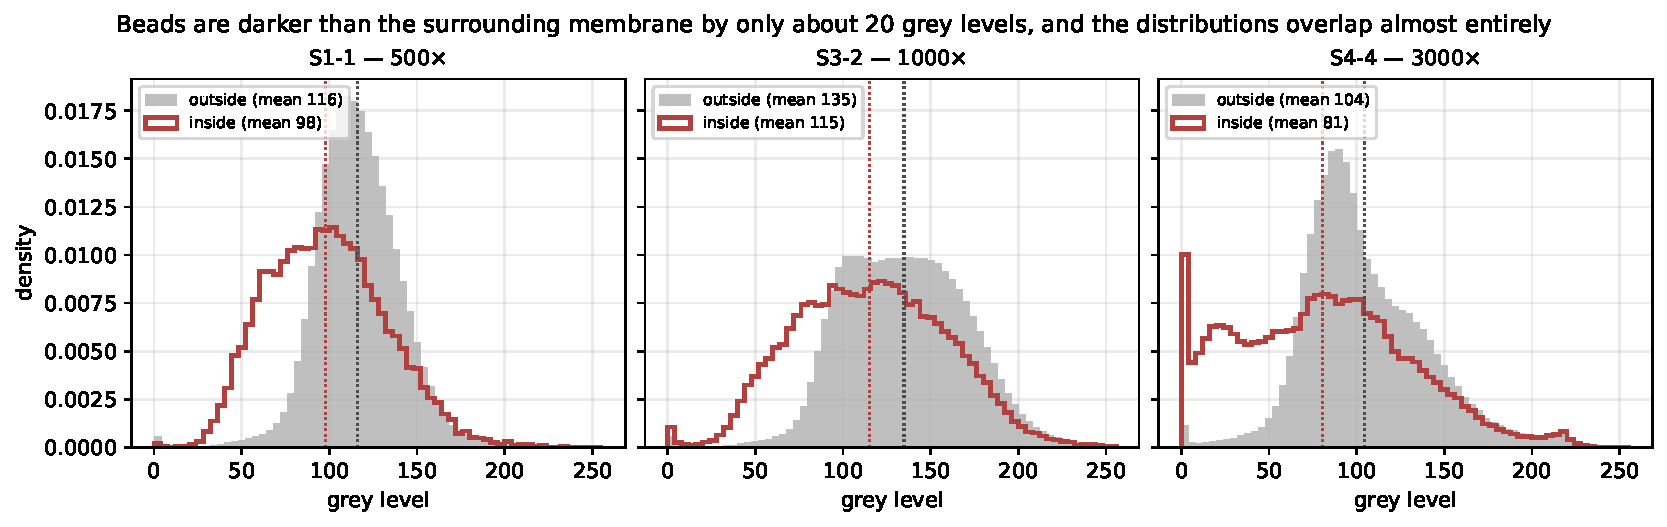
\includegraphics[width=\textwidth]{figures/fig_contrast.pdf}
    \caption{Grey-level distributions inside and outside the annotated beads, for
    one micrograph at each magnification. The means differ by about 20 levels
    while the distributions overlap almost entirely.}
    \label{fig:contrast}
\end{figure}

The parameters were tuned by grid search on the training partition of each fold
over morphological kernel size, minimum accepted object area in $\mu$m$^2$ and
marker suppression distance. The grid brackets the median annotated bead area of
about 38\,$\mu$m$^2$ from well below to well above, and the selected optimum falls
in the interior of the grid for all four folds, so the result is not an artefact
of too narrow a search. Its Segmentation Quality of 0.489 against a Recognition
Quality of 0.021 completes the picture: on the rare occasion it matches a bead the
mask is not unreasonable, but it almost never matches one.

\subsection{Method Comparison}
\label{sec:comparison}

% Generated by code/make_tables.py from results/metrics.json.
% Do not edit by hand: re-run the pipeline instead.
\begin{table}[htbp]
    \centering
    \caption{The mask-predicting methods under an identical protocol, averaged over
    the four leave-one-specimen-out folds. Counting error is the mean absolute
    percentage difference between the predicted and the annotated particle count.
    Detection-only methods are compared in Table~\ref{tab:counting}.}
    \label{tab:method_comparison}
    \begin{tabular}{lrrrr}
        \toprule
        Method & $\mathrm{AP}_{50}$ & AJI & Counting error (\%) & Merge rate (\%) \\
        \midrule
        Otsu + watershed & 0.001 & 0.067 & 580.4 & 17.4 \\
        U-Net + CC       & 0.152 & 0.305 & 44.2 & 48.7 \\
        Mask R-CNN       & 0.306 & 0.320 & 41.1 & 30.0 \\
        YOLOv8           & 0.254 & 0.254 & 93.2 & 34.5 \\
        \bottomrule
    \end{tabular}
\end{table}


Among the mask-predicting methods, Mask R-CNN leads on every metric measured and
the classical pipeline is last on all of them, so the fourth objective of
Section~\ref{sec:objectives} is met. The qualification concerns the two box-only
methods, absent from the mask-level columns. On counting, the only endpoint
defined identically for all six, Faster R-CNN is 1.7 points ahead of Mask R-CNN
(Section~\ref{sec:mask_branch}) while YOLOv5u is ahead of both on three folds and
far behind on the fourth (Section~\ref{sec:yolov5_results}). The ordering in
between depends on which metric is asked for, and that dependence is a result
rather than an inconvenience: YOLOv8 beats the U-Net on average precision, 0.254
against 0.152, and loses to it on counting, 99.3\% against 42.3\%.

The counting column separates the five failure modes more clearly than the
accuracy columns do. The classical pipeline fragments texture into objects,
over-counting by a factor of six. The U-Net fuses neighbours, under-counting by
42\% with an error entirely one-signed. YOLOv8 detects freely and fragments what
it detects, over-counting by 99\% with the highest recall and the highest split
rate, 28.5\%. YOLOv5u is the most accurate counter on three folds and the second
worst of the six on the fourth, its failure a loss of score calibration on one
specimen rather than a bias in one direction. Mask R-CNN errs in both directions:
its mean absolute counting error of 41.2\% is the lowest of the four
mask-predicting methods, while its mean signed error is $+3.0\%$, so most of its
absolute error cancels between micrographs that over- and under-count. That last
distinction matters for the application and is discussed in
Section~\ref{sec:counting}, since a method whose errors partly cancel is useful
for a population estimate in a way a biased method is not, while still being
unreliable for any single micrograph.

Table~\ref{tab:counting} restates the comparison on counting alone, the only
quantity defined identically for a method predicting masks and one predicting
only boxes. Where a row is marked \emph{box}, its average precision is computed on
bounding boxes rather than masks, and the two are not interchangeable.

% Generated by code/make_tables.py from results/metrics.json.
% Do not edit by hand: re-run the pipeline instead.
\begin{table}[htbp]
    \centering
    \caption{Counting accuracy under the leave-one-specimen-out protocol. Counts
    are pooled over the 11 held-out micrographs, while both error columns are
    averaged over them. Positive is an under-count and negative an over-count,
    and the two differ by however much the errors cancel. Methods marked (box)
    predict no masks, so their average precision is computed on boxes.}
    \label{tab:counting}
    \begin{tabular}{lrrrrr}
        \toprule
        Method & Detected & Annotated & Signed (\%) & Absolute (\%) & $\mathrm{AP}_{50}$ \\
        \midrule
        Otsu + watershed & 2205 & 606 & $-495.5$ & 502.1 & 0.001 (mask) \\
        U-Net + CC       & 325 & 606 & $+42.3$ & 42.3 & 0.152 (mask) \\
        Mask R-CNN       & 562 & 606 & $+3.0$ & 41.2 & 0.298 (mask) \\
        Faster R-CNN     & 602 & 606 & $-6.9$ & 39.5 & 0.305 (box) \\
        YOLOv8           & 1223 & 606 & $-90.2$ & 99.3 & 0.254 (mask) \\
        YOLOv5u          & 991 & 606 & $-63.0$ & 67.9 & 0.315 (box) \\
        \bottomrule
    \end{tabular}
\end{table}


Table~\ref{tab:ap_bands} decomposes average precision by object size. This matters
more here than the pooled figure suggests, since 82.8\% of the annotated particles
fall in the small band of COCO and 1.2\% in its large band
(Section~\ref{sec:small_objects}), so the pooled AP is close to an average over
a single band while appearing to describe three. $\mathrm{AP}_S$ is the column that
characterises this dataset, and it is the column that should be compared against the
small-object literature of Table~\ref{tab:coco_size} rather than against the pooled
COCO figures usually quoted.

% Generated by code/make_tables.py from results/metrics.json.
% Do not edit by hand: re-run the pipeline instead.
\begin{table}[htbp]
    \centering
    \caption{Average precision decomposed by object size, under the
    leave-one-specimen-out protocol. The bands are COCO's: small is below
    $32 \times 32$ pixels, large above $96 \times 96$. Since 82.8\% of the
    annotated particles are small and 1.2\% are large, $\mathrm{AP}_S$ is the
    column that describes this dataset; a dash marks a band the held-out ground
    truth does not populate, which cannot be scored.}
    \label{tab:ap_bands}
    \begin{tabular}{lrrrrrr}
        \toprule
        Method & AP & $\mathrm{AP}_{50}$ & $\mathrm{AP}_{75}$ &
        $\mathrm{AP}_S$ & $\mathrm{AP}_M$ & $\mathrm{AP}_L$ \\
        \midrule
        Otsu + watershed & 0.000 & 0.001 & 0.000 & --- & --- & --- \\
        U-Net + CC       & 0.049 & 0.152 & 0.031 & --- & --- & --- \\
        Mask R-CNN       & 0.113 & 0.282 & 0.069 & --- & --- & --- \\
        \bottomrule
    \end{tabular}
\end{table}


Two features of that table are worth stating. Four of the five learned methods
score higher on the medium band than on the small one, the expected direction and
the same effect Section~\ref{sec:magnification} measures against magnification;
the exception is YOLOv5u, at 0.126 against 0.132, a reversal of 0.006 belonging to
the method with the highest $\mathrm{AP}_S$ in the table. The large-band column
rests on the thinnest evidence in the chapter, since 1.2\% of the annotations are
large, fold Z4 contains none, and the column is averaged over three folds rather
than four. Nothing in this work should be concluded from it.

\subsection{Effect of Input Preprocessing}
\label{sec:preprocessing_results}

The four preprocessing variants of Section~\ref{sec:preprocessing_method} can be
characterised before any model is trained, by measuring on the annotations what
contrast each leaves available. Table~\ref{tab:contrast} reports the mean
grey-level separation between particle and mat and that separation divided by the
standard deviation of the background. The second is the one that matters, since a
transform that widens the gap while widening the spread by more has not made the
particles easier to find.

\begin{table}[htbp]
    \centering
    \caption{Particle-to-mat contrast under each preprocessing variant, measured
    over the 606 annotated particles before any training. $\Delta$ is the mean grey
    level outside a particle minus the mean inside and $\sigma$ is the background
    standard deviation.}
    \label{tab:contrast}
    \begin{tabular}{lrrrr}
        \toprule
        Preprocessing & $\Delta$ (grey levels) & $\sigma$ & $\Delta/\sigma$ &
        Change \\
        \midrule
        None (baseline)        & 18.0 & 33.2 & 0.550 & ---      \\
        Median filter, $3\times3$ & 18.3 & 30.5 & 0.612 & $+11\%$ \\
        Background subtraction & 20.3 & 34.9 & 0.593 & $+8\%$  \\
        CLAHE                  & 23.1 & 62.5 & 0.372 & $-32\%$ \\
        \bottomrule
    \end{tabular}
\end{table}

CLAHE is the instructive case. It produces the widest raw separation of the four, at
23.1 grey levels against 18.0 for the baseline, and on that number alone would be
the obvious choice. It also nearly doubles the background standard deviation, from
33.2 to 62.5, because the transform cannot distinguish a particle from the fibre
texture surrounding it and amplifies both. The usable contrast therefore falls by
almost a third. Figure~\ref{fig:preprocessing} shows this directly, as in the CLAHE
panel the fibres are as strongly modulated as the particle.

The other two transforms produce modest gains. The median filter improves
$\Delta/\sigma$ by 11\% by reducing the background spread rather than by increasing
the separation, which is the expected behaviour of a denoising filter on a signal
that it does not otherwise disturb. Background subtraction improves it by 8\%, and
its raw separation rises to 20.3, indicating that some of the measured
particle-to-mat difference in the untransformed images is attributable to
illumination gradient rather than to the particles.

\begin{figure}[htbp]
    \centering
    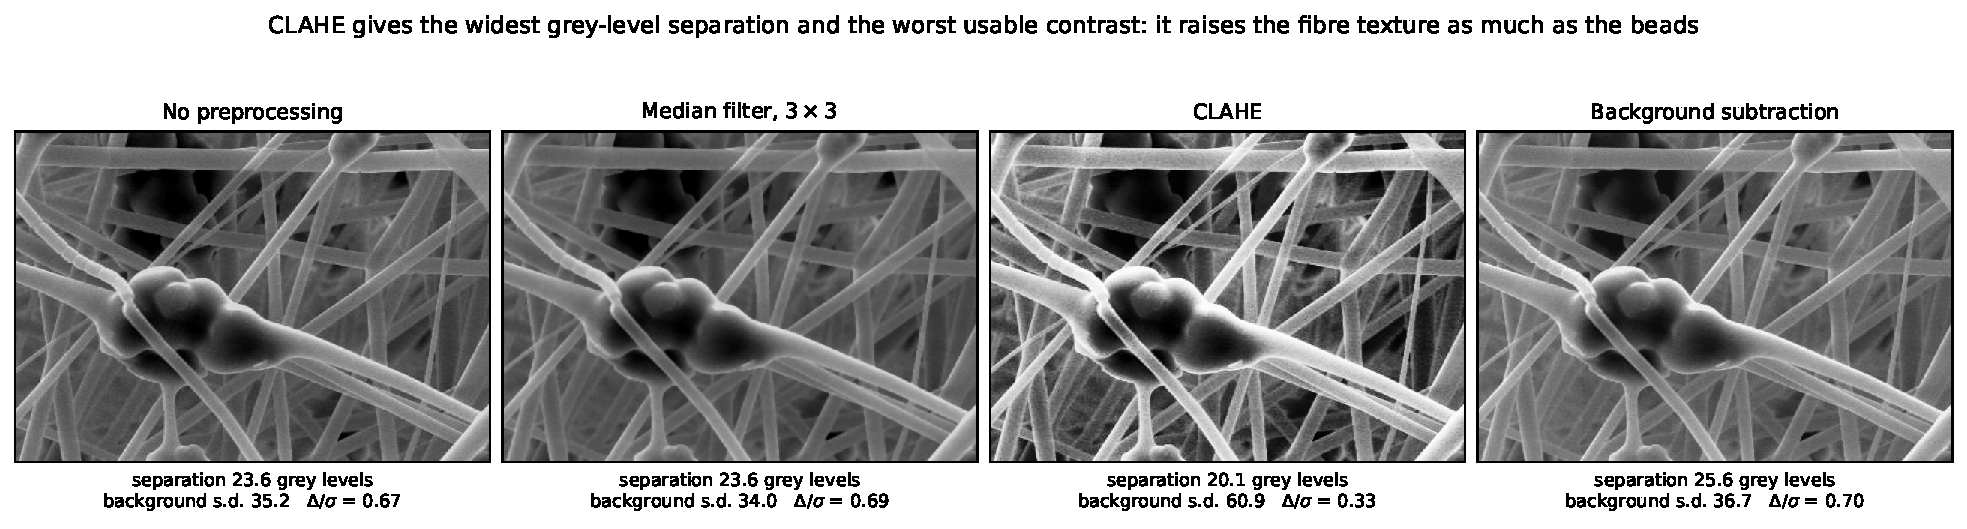
\includegraphics[width=\textwidth]{figures/fig_preprocessing.pdf}
    \caption{One region of Z6-4 under each preprocessing variant, with the
    contrast each yields over the whole dataset. In the CLAHE panel the particle is
    more strongly contrasted than in the baseline, and so is every fibre around
    it.}
    \label{fig:preprocessing}
\end{figure}

Two cautions attach to Table~\ref{tab:contrast}. It measures contrast, not
accuracy, and a convolutional detector is not a threshold, since it exploits
texture and shape this statistic ignores. And the models are initialised from
weights trained on natural images, so a transform moving the intensity statistics
far from that distribution may cost more than the contrast it buys.

% make_tables.py emits table_preprocessing.tex only when at least two variants
% have been evaluated, so this file compiles either way.
\IfFileExists{results/table_preprocessing.tex}{%
    % Generated by code/make_tables.py from results/metrics.json.
% Do not edit by hand: re-run the pipeline instead.
\begin{table}[htbp]
    \centering
    \caption{Effect of input preprocessing on Mask R-CNN, under the
    leave-one-specimen-out protocol. Architecture, schedule, folds and
    threshold-selection rule are identical across rows, so a difference is
    attributable to the input transform alone. The second column is the
    particle-to-mat contrast measured directly on the annotations before any
    training: the mean grey-level separation divided by the standard deviation of
    the background, which is the contrast a filter actually has to work with.}
    \label{tab:preprocessing}
    \begin{tabular}{lrrrrr}
        \toprule
        Preprocessing & Contrast & $\mathrm{AP}_{50}$ & $\mathrm{AP}_S$ &
        AJI & Counting error (\%) \\
        \midrule
        None (baseline)            &  0.55 & 0.306 & 0.116 & 0.320 & 41.1 \\
        Median filter, 3x3         &  0.61 & 0.289 & 0.108 & 0.320 & 36.4 \\
        CLAHE                      &  0.37 & 0.262 & 0.094 & 0.290 & 39.3 \\
        Background subtraction     &  0.59 & 0.263 & 0.104 & 0.307 & 31.3 \\
        \bottomrule
    \end{tabular}
\end{table}
%
}{}

\textbf{No transform improves detection over the untransformed input.} Mask R-CNN
scores $\mathrm{AP}_{50} = 0.298$ on the raw micrographs, against 0.289 with the
median filter, 0.263 with background subtraction and 0.262 with CLAHE, and the
ordering on $\mathrm{AP}_S$ is the same; architecture, schedule, folds and
threshold-selection rule were identical across the four rows. The contrast
statistic therefore succeeded at one of its two jobs: it identified the harmful
transform correctly, since CLAHE loses a third of the usable contrast and is last
or joint-last on every accuracy column, but failed to identify a beneficial one,
having predicted gains of 11\% and 8\% for the median filter and background
subtraction, both of which cost detection accuracy instead. The two cautions
recorded above, before the runs rather than after them, are the likeliest
explanation.

One row points the other way, and it is the row the laboratory cares about most.
Background subtraction gives the lowest counting error of the four variants,
31.5\% against 41.2\%, while losing 0.035 of $\mathrm{AP}_{50}$, and it has the
lowest split rate of any Mask R-CNN variant, 11.6\% against 13.8\%. What separates
the two on counting is not the average instance behaviour but the tails: the two
worst frames of the baseline over-count by 119\% and 83\%, and background
subtraction brings them to 27\% and 21\%, at the cost of turning a near-miss on
the densest micrograph into a 50\% under-count. The reading this supports is
narrow. Removing the illumination gradient does not help the detector find beads
and on this evidence slightly hinders it; what it does is suppress the runaway
over-counts on sparsely populated frames, which is what a mean of per-micrograph
percentage errors rewards most. These runs cannot say which difference would
survive a second seed (Section~\ref{sec:reliability}).

\subsection{Effect of Threefold Magnification}
\label{sec:upsample_results}

Section~\ref{sec:magnification} finds that the model detects best where the beads
occupy the most pixels. That finding suggests an intervention that costs nothing in
acquisition, namely resampling the dataset itself. Each micrograph and its
annotation are magnified threefold with bicubic interpolation, the network is
trained and run at the magnified scale, and its predictions are mapped back to
native resolution before scoring, so both configurations are measured against
the same ground truth in the same coordinate frame.

% Emitted only when the magnified run has been evaluated.
\IfFileExists{results/table_upsample.tex}{%
    % Generated by code/make_tables.py from results/metrics.json.
% Do not edit by hand: re-run the pipeline instead.
\begin{table}[htbp]
    \centering
    \caption{Effect of magnifying the dataset threefold by bicubic
    interpolation, under the leave-one-specimen-out protocol. Image and
    annotation are resampled together and the predictions are mapped back to
    native resolution before scoring, so both rows are measured against the same
    ground truth. Architecture, schedule, folds and threshold-selection rule are
    identical.}
    \label{tab:upsample}
    \begin{tabular}{lrrrr}
        \toprule
        Input scale & $\mathrm{AP}_{50}$ & $\mathrm{AP}_S$ & AJI &
        Counting error (\%) \\
        \midrule
        Native resolution            & 0.298 $\pm$ 0.059 & 0.116 & 0.325 $\pm$ 0.053 & 41.1 \\
        $3\times$ bicubic            & 0.373 $\pm$ 0.039 & 0.158 & 0.359 $\pm$ 0.052 & 42.7 \\
        \bottomrule
    \end{tabular}
\end{table}
%
}{}

The effect is the largest of any input-side intervention reported here.
$\mathrm{AP}_{50}$ rises from 0.298 to 0.373 and $\mathrm{AP}_S$ from 0.116 to
0.158, gains of 0.075 and 0.042 against a between-fold standard deviation of 0.059
and 0.035 respectively. AJI rises from 0.325 to 0.359 and Panoptic Quality from
0.351 to 0.394, and the decomposition says where the gain comes from: Recognition
Quality rises from 0.486 to 0.541 while Segmentation Quality moves only from 0.719
to 0.733. Pooled over the 11 held-out micrographs the model now matches 397 of the
606 annotated beads against 271 before, a recall of 0.655 against 0.447, at an
essentially unchanged precision of 0.493 against 0.482.

Interpolation adds no information, and the result should not be read as though it
did. What changes is the number of pixels per object: the median bead at
$500\times$ goes from 14 pixels across to 42, moving it from the size at which the
finest pyramid level and the smallest anchor are both marginal to one at which
neither is. The gain is therefore evidence for the diagnosis of
Section~\ref{sec:magnification}, obtained by changing only the scale of the input.

The counting endpoint does not follow. Mean absolute counting error is 44.0\%
against 41.2\%, and the aggregate turns from a deficit into a surplus, 806 objects
against 606 annotated where the baseline reported 562. Finding more beads has
meant fragmenting more of them, the split rate rising from 13.8\% to 18.0\% and
the merge rate from 24.9\% to 28.9\%, which is the same trade the instance methods
make against each other in Section~\ref{sec:comparison}, reappearing within one
architecture.

The cost is not negligible. Training takes 26.3 minutes per fold against 10.3, and
inference has to be tiled, since a magnified micrograph is $3072 \times 2208$ and
the mask head allocates one full-resolution mask per detection. For a laboratory
whose endpoint is the size distribution the gain is worth two and a half times the
training time; for one whose endpoint is the count, this run offers nothing.

\subsection{Qualitative Examples}

\begin{figure}[htbp]
    \centering
    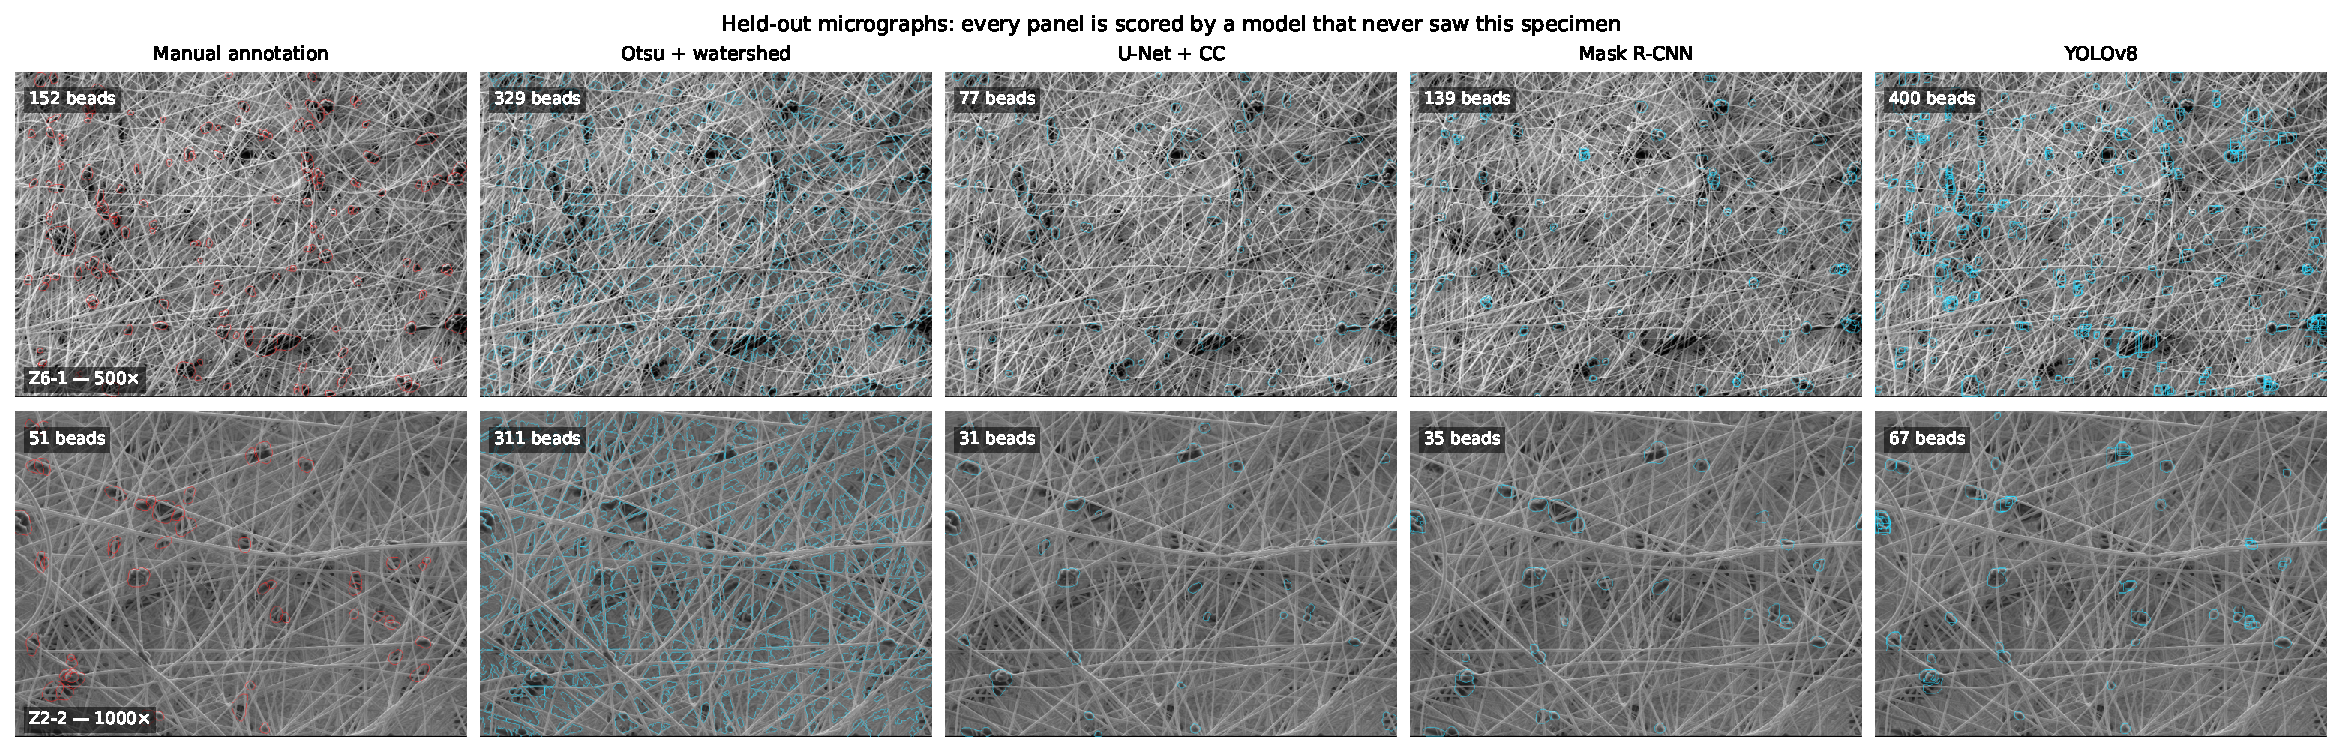
\includegraphics[width=\textwidth]{figures/fig_qualitative.pdf}
    \caption{The four mask-predicting methods on two held-out micrographs, Z6-1
    at $500\times$ and Z2-2 at $1000\times$, each from a model that never saw that
    specimen. Red outlines are the manual annotation, blue the prediction. Faster
    R-CNN predicts no masks and is absent.}
    \label{fig:qualitative}
\end{figure}

Figure~\ref{fig:qualitative} shows the mask-predicting methods on two held-out
micrographs, and each numerical finding above has a visible counterpart in it.

On Z6-1 the annotator marked 152 beads. The classical pipeline returns 329 regions
that tile the frame more or less irrespective of where the beads are, which is the
visual form of an $\mathrm{AP}_{50}$ of 0.001. The U-Net returns 77 regions, half
the true count, visibly larger than individual beads because adjacent beads have
been absorbed into single components: the 48.7\% merge rate made visible. YOLOv8
returns 400, hitting the detection cap, with many small outlines subdividing
single annotated beads. Mask R-CNN returns 139 regions that correspond
recognisably to individual beads, and its errors are of a different kind, beads
missed entirely rather than fused or fragmented. On Z2-2, where the annotator
marked 51 beads, the same pattern holds at a different scale: the classical
pipeline returns 311 regions, the U-Net 31 and Mask R-CNN 35, both under-counting
although the U-Net's regions again span neighbouring beads, while YOLOv8 returns
67.

\section{The Cost of a Naive Split}
\label{sec:leakage}

% Generated by code/make_tables.py from results/metrics.json.
% Do not edit by hand: re-run the pipeline instead.
\begin{table}[htbp]
    \centering
    \caption{The same model under a specimen-wise protocol and under a random
    split over the 11 images, with identical fold sizes.}
    \label{tab:leakage}
    \begin{tabular}{lrrr}
        \toprule
        Protocol & $\mathrm{AP}_{50}$ & AJI & Counting error (\%) \\
        \midrule
        Random split over images & 0.303 & 0.313 & 43.9 \\
        Leave-one-specimen-out   & 0.298 & 0.325 & 41.2 \\
        \midrule
        Difference & 0.005 & -0.012 & 2.7 \\
        \bottomrule
    \end{tabular}
\end{table}


This is a negative result and it is reported as measured.

Evaluating the same model under a random split over the 11 micrographs, with fold
sizes identical to the specimen-wise protocol, gives
$\mathrm{AP}_{50} = 0.303$ against 0.298 for leave-one-specimen-out, a difference
of 0.005 in favour of the random split, against a between-fold standard deviation
of 0.059. The other two metrics run the other way, as AJI is 0.313 against 0.325
and mean absolute counting error 43.9\% against 41.2\%. Only one of the three
differences points in the direction a leak would produce, and it is a twelfth of
the between-fold spread. On this dataset the naive protocol does not measurably
overstate performance.

The second objective of Section~\ref{sec:objectives} asked for a demonstration
that the naive alternative overstates performance, and that demonstration did not
materialise. The protocol remains the correct one, but on the strength of
structural argument rather than of measured inflation. Three factors plausibly
explain the absence of a gap, and the first is the most likely.

\textbf{The leak that mattered had already been removed.} The 132 pre-computed
augmented copies were discarded before any partitioning
(Section~\ref{sec:supplied_aug}). They are near-duplicates of their originals, so
letting them cross a partition boundary would put a transformed version of a test
image directly into training. The remaining dependence between two micrographs of
one specimen at different magnifications is far weaker, being different fields of
view at different scales that share only the general morphology of the specimen.

\textbf{There is little headroom to inflate.} A protocol can only flatter a model
capable of memorising. At $\mathrm{AP}_{50} = 0.30$ and a Recognition Quality of
0.49, this model is under-fitting rather than memorising, and
Section~\ref{sec:generalisation} measures that directly.

\textbf{With 11 images, both protocols are noisy.} The folds of the random split
range from $\mathrm{AP}_{50} = 0.199$ to 0.423, a spread of 0.224, against 0.223
to 0.355 for the specimen-wise folds, a spread of 0.132. The random protocol gave
a mean higher by 0.005 and a fold-to-fold spread 1.7 times as wide, which is
reason to prefer the specimen-wise protocol independently of any bias argument: it
is the more stable estimator, and on four folds stability is worth more than it
would be on forty.

\section{Training Accuracy against Test Accuracy}
\label{sec:generalisation}

Section~\ref{sec:leakage} argues that there is little headroom for a protocol to
inflate, because the model is under-fitting rather than memorising. That argument
can be measured. The model of each fold is scored a second time on the eight
micrographs on which it was trained, by the same code and against the same
annotations.

% Emitted only when at least one method has recorded a training partition.
\IfFileExists{results/table_generalisation.tex}{%
    % Generated by code/make_tables.py from results/metrics.json.
% Do not edit by hand: re-run the pipeline instead.
\begin{table}[htbp]
    \centering
    \caption{Training accuracy against test accuracy under the
    leave-one-specimen-out protocol. Each fold's model is scored on the
    micrographs it was trained on and on the specimen it was held out from, by
    the same code and against the same annotations. The gap is train minus test
    in each metric's own units, so the model favours what it has already seen
    when the $\mathrm{AP}_{50}$ gap is positive and when the counting gap is
    negative. The training figure is not a result in
    its own right -- it is measured on data the optimiser was given -- but the
    distance between the two columns is: it separates a model that has memorised
    its training specimens from one that is limited by the difficulty of the
    task. No pooled figure is given because a micrograph belongs to the training
    partition of three of the four folds, so pooling would weight specimens by
    how often they recur.}
    \label{tab:generalisation}
    \begin{tabular}{lrrrrrr}
        \toprule
        & \multicolumn{3}{c}{$\mathrm{AP}_{50}$} &
        \multicolumn{3}{c}{Counting error (\%)} \\
        \cmidrule(lr){2-4} \cmidrule(lr){5-7}
        Method & Train & Test & Gap & Train & Test & Gap \\
        \midrule
        Mask R-CNN               & 0.437 & 0.298 & +0.139 & 32.6 & 41.1 & -8.5 \\
        Faster R-CNN             & 0.412 & 0.305 & +0.107 & 35.7 & 37.8 & -2.2 \\
        Mask R-CNN, $3\times$ bicubic & 0.459 & 0.373 & +0.086 & 46.0 & 42.7 & +3.3 \\
        \bottomrule
    \end{tabular}
\end{table}
%
}{}

The gap is real and modest. Mask R-CNN scores $\mathrm{AP}_{50} = 0.437$ on data
it has seen against 0.298 on data it has not. The ratio is the wrong way to read
it: what matters is that 0.437 is itself a modest score, so the model does not
come close to fitting even its training partition. A network that had memorised
eight micrographs would score near ceiling on them and this one does not, so the
deficit reported throughout the chapter is one of capacity and training budget
rather than of generalisation.

Two comparisons within the table sharpen that. Faster R-CNN, the same architecture
with the mask head removed, has a smaller gap than Mask R-CNN, 0.107 against
0.139, the expected direction for a model with fewer parameters to fit. The
threefold-magnified model has the smallest gap of the three, 0.086, together with
the highest test score, so its gain is not bought by fitting the training data
harder, which is what a resampling artefact would have looked like.

The counting column is reported for completeness. Mask R-CNN counts better on its
training partition than on its test specimen, 32.5\% against 41.2\%, Faster R-CNN
barely distinguishes the two, 35.7\% against 39.5\%, and the magnified model
counts \emph{worse} on training than on test, 45.6\% against 44.0\%. That
inversion is not a paradox, since the counting figure is an unweighted mean of
per-micrograph percentage errors dominated by the sparsely populated frames. The
training column is not a result in its own right, and it is optimistic twice over,
since the score threshold was itself chosen by maximising $F_1$ on that same
partition. No pooled training figure is given, because a micrograph belongs to the
training partition of three folds.

\section{Behaviour Across Magnification}
\label{sec:magnification}

% Generated by code/make_tables.py from results/metrics.json.
% Do not edit by hand: re-run the pipeline instead.
\begin{table}[htbp]
    \centering
    \caption{Mask R-CNN performance by magnification, pooled over the four
    leave-one-specimen-out folds. Every micrograph is scored by the model that
    did not see its specimen.}
    \label{tab:magnification}
    \begin{tabular}{lrrrrr}
        \toprule
        Magnification & Images & Beads & $\mathrm{AP}_{50}$ & AJI & $|$Counting error$|$ (\%) \\
        \midrule
        $500\times$ & 3 & 325 & 0.227 & 0.233 & 29.1 \\
        $1000\times$ & 4 & 229 & 0.342 & 0.316 & 48.8 \\
        $3000\times$ & 4 & 52 & 0.396 & 0.384 & 42.6 \\
        \bottomrule
    \end{tabular}
\end{table}


Detection improves monotonically with magnification, the opposite of what the
sample sizes alone would predict. The $3000\times$ group is the smallest in the
dataset, 52 beads across four micrographs against 325 at $500\times$, and is
nonetheless the group on which the model detects best, at
$\mathrm{AP}_{50} = 0.396$ and AJI 0.384 against 0.227 and 0.233 at $500\times$.

Object size and not sample size is therefore the binding constraint. The median
bead is 14 pixels across at $500\times$ and 76 at $3000\times$. At 14 pixels a
bead spans roughly the receptive field of the finest pyramid level and is only a
few pixels larger than the smallest anchor, so its boundary is decided by a
handful of pixels, whereas at 76 pixels it is comfortably resolved.
Table~\ref{tab:magnification} shows that the feature pyramid and the rescaled
anchors narrow the gap without closing it.

Counting does not follow the same ordering. The mean absolute counting error is
lowest at $500\times$, 29.1\%, and higher at both other settings, 48.8\% at
$1000\times$ and 42.6\% at $3000\times$. Part of that is an arithmetic property of
the field of view rather than a contradiction of the detection result, since a
$3000\times$ micrograph carries 13 annotated beads on average and as few as four,
so one spurious detection on a four-bead frame is a 25\% error while one on the
152-bead Z6-1 is 0.7\%. The ordering between $1000\times$ and $3000\times$ is not
evidence of anything: each group holds three or four micrographs and the mean of
each is dominated by one of them, the 48.8\% at $1000\times$ carried by Z6-2,
over-counted by 119\%, and the 29.1\% at $500\times$ by Z5-1, under-counted by
75\%, so removing either frame reverses the ranking. The detection columns, which
average over hundreds of objects, are the ones this table supports.

The practical consequence follows from the detection trend alone. High
magnification gives better boundaries and therefore a better size distribution. If
both quantities are wanted from one setting, $1000\times$ is the defensible
compromise, within 0.054 of the best $\mathrm{AP}_{50}$ while framing 229
annotated beads against the 52 available at $3000\times$. What these results
cannot support is a recommendation based on the counting column itself, and with
only 52 beads the $3000\times$ figures should be read as indicative.

\section{Physical Quantification}

\subsection{Bead Count and Areal Density}
\label{sec:counting}

Summed over all 11 held-out micrographs, Mask R-CNN reports 562 beads against 606
annotated, an aggregate under-count of $+7.3\%$. That figure is far more
favourable than the method deserves, since it is the sum of errors that largely
cancel. Per specimen the mean signed error runs from $+40.3\%$ on Z4, the largest
under-count, to $-64.7\%$ on Z6, the largest over-count, and per micrograph from
$+74.5\%$ on Z5-1 to $-119.4\%$ on Z6-2, while the mean absolute error is 41.2\%
against a mean signed error of $+3.0\%$. A single micrograph is therefore not a
reliable measurement, and 7.3\% against 41.2\% is a factor of six, none of which
comes from the model being right.

That cancellation is a property of the method rather than of aggregation. Faster
R-CNN aggregates to $+0.7\%$ against a mean absolute error of 39.5\%, a wider gap
still. YOLOv5u gains nothing, its aggregate of $-63.5\%$ nearly matching its mean
absolute error because its error is one-signed and concentrated on a single
specimen, while the aggregate of $-101.8\%$ for YOLOv8 is worse than its mean
absolute error of 99.3\%. A
laboratory pooling many micrographs would gain roughly a factor of six from Mask
R-CNN, more from Faster R-CNN, and nothing from either YOLO model. That
distinction appears in no accuracy column in this chapter.

Figure~\ref{fig:counting} plots the two counts against each other. Four of the
eleven micrographs fall within 25\% of the annotated count, and the largest errors
lie on both sides: Z5-1, the second most densely populated micrograph, is
under-counted by three quarters, while Z6-2 is over-counted by 119\% and Z6-4 by
83\%. The extremes are at both ends of the density range, which is where a merge
on the dense frames, or a spurious split on the sparse ones, costs most.

\begin{figure}[htbp]
    \centering
    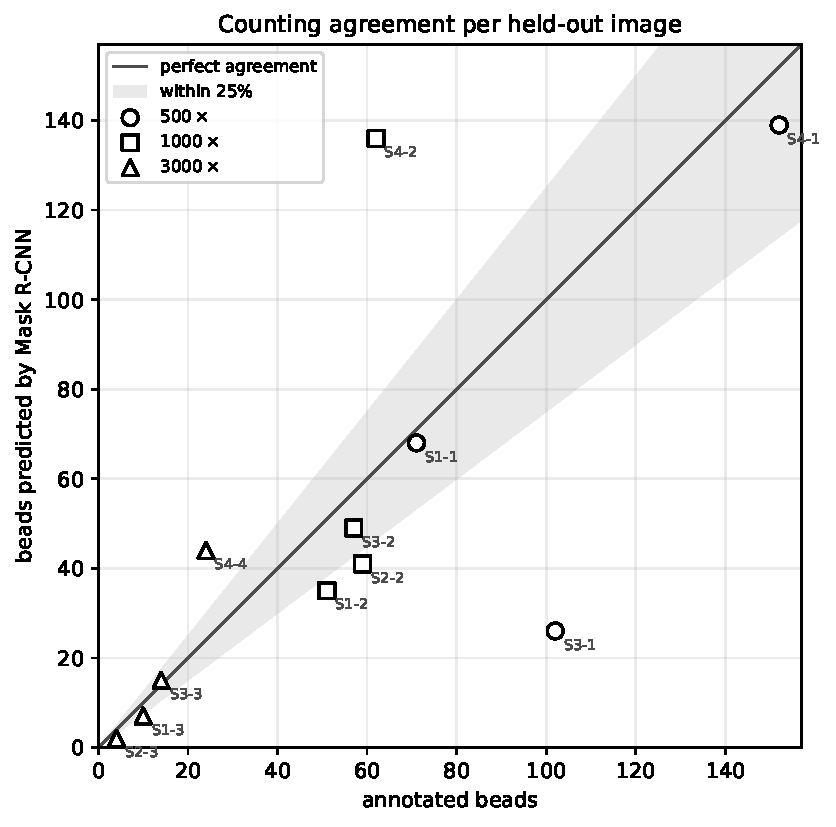
\includegraphics[width=0.78\textwidth]{figures/fig_counting.pdf}
    \caption{Predicted against annotated bead count for each held-out micrograph,
    with marker shape indicating magnification. Points on the diagonal agree
    exactly.}
    \label{fig:counting}
\end{figure}

Areal density inherits this behaviour directly, since it is the count divided by a
known physical area. On Z2-1 the model reports 292 beads\,mm$^{-2}$ against 305
measured manually, on Z5-1 it reports 112 against 438, and on Z6-2, 2338 against
1066. The fifth objective of Section~\ref{sec:objectives} is met in the sense that
these quantities are reported and compared, but the comparison does not support
using the pipeline as a drop-in replacement for manual counting on a single field.

\subsection{Size Distribution Agreement}

% Generated by code/make_tables.py from results/metrics.json.
% Do not edit by hand: re-run the pipeline instead.
\begin{table}[htbp]
    \centering
    \caption{Predicted bead size distribution against the manual ground truth,
    pooled over the 11 held-out micrographs. Diameters are equivalent circular
    diameters in micrometres.}
    \label{tab:physical}
    \begin{tabular}{lrrrrr}
        \toprule
        Source & Beads & Median $d$ ($\mu$m) & IQR ($\mu$m) & KS $D$ & $p$ \\
        \midrule
        Manual annotation & 606 & 7.97 & [6.42, 10.16] & --- & --- \\
        \midrule
        Otsu + watershed & 2205 & 8.58 & [6.72, 10.99] & 0.105 & 4.9e-05 \\
        U-Net + CC       & 325 & 8.78 & [6.48, 12.09] & 0.154 & 7.5e-05 \\
        Mask R-CNN       & 562 & 7.72 & [5.65, 9.14] & 0.139 & 2.4e-05 \\
        YOLOv8           & 1223 & 7.81 & [6.05, 10.39] & 0.075 & 2.0e-02 \\
        \bottomrule
    \end{tabular}
\end{table}


The predicted median diameter of Mask R-CNN is 7.72\,$\mu$m against 7.97\,$\mu$m
measured manually, a difference of 3.2\%, with an interquartile range of 5.65 to
9.14\,$\mu$m against 6.42 to 10.16\,$\mu$m. The predicted distribution is narrower
and smaller, consistent with a detector that misses the beads hardest to delineate
and trims the boundaries of those it keeps.

All four two-sample Kolmogorov--Smirnov tests reject the hypothesis that the
predicted and manual distributions are the same, three at $p < 10^{-3}$ and that
of YOLOv8 at $p = 0.02$. That should not be over-read, since with hundreds of
samples on each side the test is sensitive to differences far smaller than those
that matter for process optimisation, and a 3.2\% error in median bead diameter is
smaller than the 15\% spread the same annotation shows across magnifications.
Figure~\ref{fig:size_agreement} shows that Mask R-CNN tracks the manual
distribution closely through its bulk and falls short in the tail above roughly
15\,$\mu$m.

\begin{figure}[htbp]
    \centering
    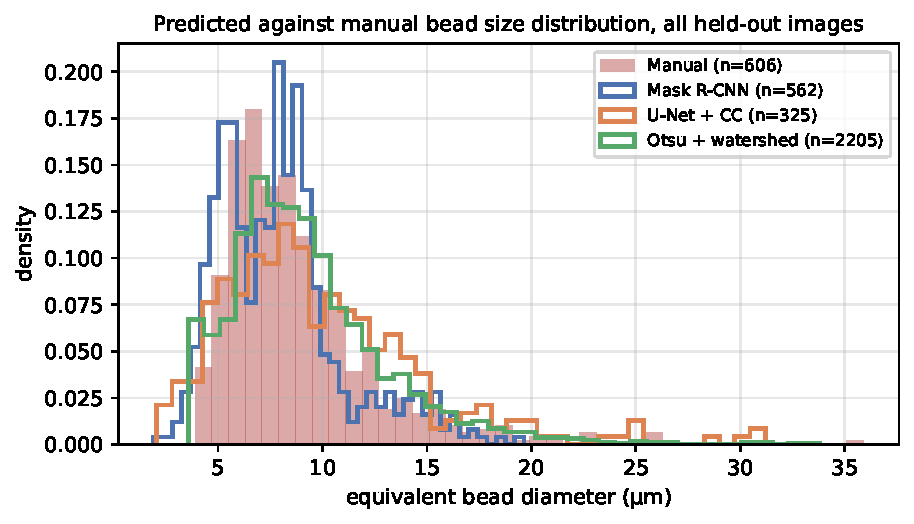
\includegraphics[width=0.9\textwidth]{figures/fig_size_agreement.pdf}
    \caption{Predicted against manual bead size distributions, pooled over all
    11 held-out micrographs.}
    \label{fig:size_agreement}
\end{figure}

Two rows of Table~\ref{tab:physical} are a warning rather than a finding. Of the
four methods, YOLOv8 has the \emph{lowest} KS statistic at $D = 0.075$ and the
classical pipeline the second lowest at $D = 0.105$, and these are the two that
over-count by 99\% and 495\%. Both achieve their agreement by reporting far more
objects than exist, whose sizes happen to span a similar range to the real beads,
while Mask R-CNN, the best method by every other measure here, has a worse $D$ than
both.

Distributional agreement alone is therefore not a sufficient criterion, since a
method can reproduce the size distribution of a population that it has substantially
failed to identify. Had this work reported only the size distribution, which is one
of the two quantities that the laboratory asked for, it would have ranked the two
worst methods first.

\section{Discussion}

\subsection{Key Findings}

\textbf{Instance segmentation is the right formulation, and the reason is
separation rather than accuracy.} Mask R-CNN and the U-Net differ by 0.020 in AJI
but by 0.157 in Panoptic Quality and by 23.8 percentage points in merge rate, and
the annotation itself contains 8.8\% overlapping bead pixels. The formulation
trades one error for another rather than eliminating error: the U-Net merges
48.7\% of beads and splits none, Mask R-CNN merges 24.9\% and splits 13.8\%, and
YOLOv8 merges 34.5\% and splits 28.5\%.

\textbf{Counting can be far more accurate than the mean figures suggest, and the
obstacle is score calibration rather than detection.} YOLOv5u counts three of the
four held-out specimens to within 8.2\%, 15.0\% and 18.3\% and misses the fourth
by 212.5\%, mostly because the training partition set a threshold of 0.10 on that
fold against 0.20 to 0.35 on the others.

\textbf{Small objects, not scarce labels, are the binding constraint on
detection.} Detection is best where the data are scarcest and the objects largest,
and magnifying the dataset threefold raises $\mathrm{AP}_{50}$ from 0.298 to 0.373
and recall from 0.447 to 0.655 without adding information, which is precisely why
it is evidence. The model under-fits rather than memorises, reaching 0.437 on the
micrographs it trained on, so the shortfall is one of capacity and training budget.

\textbf{The absolute performance is not yet sufficient for unattended use.} An
$\mathrm{AP}_{50}$ of 0.298 and a per-micrograph counting error of 41.2\% do not support
replacing a human operator on a single micrograph, although the aggregate error
over eleven micrographs is 7.3\%. Classical thresholding is not viable at all, at
$\mathrm{AP}_{50} = 0.001$, for a reason measurable in the micrographs: about 20
grey levels separate a bead from the surrounding mat.

\textbf{Preprocessing did not improve detection, and one variant improved
counting.} No transform beat the raw input on $\mathrm{AP}_{50}$, while background
subtraction cut counting error from 41.2\% to 31.5\%. And the specimen-wise
protocol did not change the headline number, but reduced the fold-to-fold spread
by a third, which is a weaker claim than the one anticipated in
Section~\ref{sec:objectives} and the one the data support.

\subsection{Comparison with the Literature}

A direct numerical comparison with published work is not possible, since no public
benchmark for beads in electrospun mats exists and the AP values reported
here are specific to this annotation and protocol. Three qualitative comparisons
can be made.

The merge behaviour of semantic segmentation with connected-component
post-processing is well documented in the nuclei segmentation literature, and
motivates the shape-prior methods of Schmidt et al.\ \cite{schmidt2018stardist}
and Stringer et al.\ \cite{stringer2021cellpose} and the weighted-boundary loss of
the original U-Net \cite{ronneberger2015unet, falk2019unet}. The 48.7\% merge rate
measured here is a direct instance of that effect.

The difficulty of small objects for region-based detectors is likewise a known
property of the architecture, and is what the feature pyramid
\cite{lin2017feature} was introduced to address. The one-stage weakness on small
objects reported for the YOLO family \cite{redmon2016yolo, lin2020focal} appears
in one of the two models tested and not the other: YOLOv8 reaches an
$\mathrm{AP}_S$ of 0.091 against 0.116 for Mask R-CNN, while YOLOv5u reaches
0.132, the highest of the six. At this object size the weakness is therefore not a
property of the family as such, and four folds cannot establish whether the
backbone or the mask branch accounts for the gap.

The absolute values are well below those reported on nuclei benchmarks such as the
dataset of Kumar et al.\ \cite{kumar2017dataset}, and the relevant difference is
training set size: those results rest on tens of thousands of annotated objects
against 606 here from four specimens.

\subsection{Limitations}
\label{sec:limitations}

The limitations below follow from the dataset and from the experimental design.

\textbf{Four specimens.} The strongest claim this dataset can support is
generalisation across four specimens of what appears to be one material system. It
cannot establish generalisation to a different polymer, solvent or instrument.

\textbf{Fifty-two beads at $3000\times$.} The highest magnification is represented
by only 52 annotated objects, so the per-magnification result for $3000\times$,
which is also the most striking finding of Section~\ref{sec:magnification}, rests
on a small sample and should be read as indicative.

\textbf{One annotator.} All 606 annotations come from a single source, so
annotator bias cannot be distinguished from ground truth and no inter-annotator
agreement can be reported. At $\mathrm{AP}_{50} = 0.298$ it is not known how much
of the shortfall is model error and how much is disagreement that a second
annotator would also show.

\textbf{Single class.} The annotation does not distinguish beads from locally
thickened fibre segments, so the boundary between the two rests on the implicit
judgement of the annotator. Several of the false positives on visual inspection
are objects of this ambiguous kind.

\textbf{No hyperparameter search.} Every model was trained once, with the
configuration of Table~\ref{tab:training_config}, for 1500 iterations. The
reported figures are what that configuration produces and not the best achievable.

\textbf{Neither YOLO model was given a matched input budget.} Both were trained on
whole $1024$-pixel micrographs where the region-based models saw
$512 \times 512$ crops, because their data pipeline expects a fixed image
directory. Their accuracy figures are therefore not a like-for-like architectural
comparison, and their threefold training cost is largely a consequence of that
difference.

\textbf{The detection cap binds for YOLOv8 on one micrograph.} It returns exactly
400 objects on Z6-1, so its over-count there, and hence its pooled counting error,
is a lower bound rather than a measurement. It does not bind for any other method,
the largest output of YOLOv5u on the same micrograph being 292.

\textbf{The YOLOv5u counting figure averages two different behaviours.} Its mean
of 67.9\% describes neither, since three folds fall between 8.2\% and 18.3\% and
the fourth at 212.5\%. The threshold diagnostic of
Section~\ref{sec:yolov5_results} is labelled a diagnostic for the same reason, as
it re-scores held-out predictions.

\subsection{Reliability of the Reported Numbers}
\label{sec:reliability}

Each configuration was run \emph{once}, with a fixed seed of 0. No seed was varied
and no configuration was repeated, so every figure in this chapter is a single-run
point estimate and none of the reported standard deviations measures run-to-run
variability. They are between-fold spreads over four folds, which is a different
and weaker quantity: they describe how much the result depends on which specimen
was held out. Counting error is the exception, summarised over the eleven
micrographs rather than the four folds; a between-fold spread of it is named as
such where one is quoted.

With four folds, a standard deviation is itself estimated from four numbers and is
not a confidence interval. Varoquaux \cite{varoquaux2018crossvalidation} shows
that cross-validated estimates from small samples carry error bars far wider than
is usually assumed, and that differences well below them are routinely reported as
findings. Two comparisons here are the most exposed. The protocol comparison of
Section~\ref{sec:leakage} turns on 0.005 in $\mathrm{AP}_{50}$, about a twelfth of
the between-fold spread, so the correct reading is that no difference was detected
rather than that the protocols were shown equivalent. The preprocessing comparison
turns on differences of 0.009 to 0.036 against a spread of 0.059, where the
direction is consistent across the three variants but no single pairwise
difference is resolved.

The magnification ablation of Section~\ref{sec:upsample_results} is the one
input-side comparison not in that position. Its gain of 0.075 in
$\mathrm{AP}_{50}$ exceeds the between-fold standard deviation of the baseline and
holds on three folds, by 0.059, 0.181 and 0.096 on Z2, Z5 and Z6. The exception is
Z4, where the magnified model scores 0.317 against 0.355, this being the fold of
63 beads across two micrographs. These runs resolve that difference in the sense
that its size exceeds the noise, but cannot put an interval on it.

What can be stated robustly is the ranking of the classical pipeline against the
learned methods, consistent across every metric and every fold; the direction and
magnitude of the merge, split and counting biases, which are large and
systematically signed; and the factor of six between per-micrograph and aggregate
counting error. What cannot is any small difference between two similar numbers,
including the ordering of Mask R-CNN against YOLOv8 on average precision and that
of YOLOv5u against Faster R-CNN, where 0.315 against 0.305 is set against
between-fold spreads of 0.049 and 0.073.

\section{Summary}

Mask R-CNN leads the mask-predicting alternatives on every metric, at
$\mathrm{AP}_{50} = 0.298 \pm 0.059$, AJI $0.325 \pm 0.053$ and a counting error
of 41.2\%, and reaches neither criterion of Section~\ref{sec:objectives}. The
comparison locates what the instance formulation contributes, the separation of
touching objects rather than mask accuracy, and what it does not: the mask branch
is worth every mask-level measurement and nothing on the count, while the two
box-only methods clear the 0.30 criterion on the quantity it was originally
measured on. YOLOv5u counts three specimens better than anything else here and the
fourth far worse, for a reason that is score calibration rather than detection.

On the input side, object size in pixels is the binding constraint: detection
improves with magnification although the highest magnification holds the fewest
beads, and resampling the dataset threefold reproduces the gain without adding
information. No preprocessing variant improved detection, one improved counting,
and the naive partitioning protocol did not measurably overstate performance.
Predicted bead diameters agree with the manual measurement to 3.2\% in the median,
while counting remains too variable per micrograph, 41.2\% against an aggregate
7.3\% over eleven, for unattended use.

\chapter{CONCLUSION AND FUTURE WORK}
\label{ch:conclusion}

\section{Conclusion}

This thesis addressed the automated quantification of bead defects in SEM
micrographs of electrospun nanofibre mats, a measurement currently performed by
hand and therefore slow and difficult to reproduce.

The dataset work is reported in Chapter~\ref{ch:methodology}. Eleven micrographs
of four specimens at three magnifications, carrying 606 manually delineated
beads, were characterised and placed on a physical scale from each micrograph's
burned-in scale bar, and the calibration was validated against the data
themselves: the median equivalent bead diameter agrees to within 15\% across the
three magnifications, which holds only if calibration and annotation are both
consistent.

Two properties of the dataset determine how it must be used. The 143
image--annotation pairs supplied are 11 originals and 132 transformed copies, so
the effective sample size is 11 and the copies cannot cross a partition boundary;
and the eleven micrographs derive from only four specimens, so the specimen
rather than the image is the unit of partitioning. Both are reflected in the
leave-one-specimen-out protocol adopted throughout.

Under that protocol, Mask R-CNN outperforms the mask-predicting alternatives on
every metric measured, reaching $\mathrm{AP}_{50} = 0.298 \pm 0.059$, an
Aggregated Jaccard Index of $0.325 \pm 0.053$ and a mean absolute counting error
of 41.1\%. It reaches neither success criterion of Section~\ref{sec:objectives}:
far short of the $\mathrm{AP}_{50} \geq 0.70$ recorded at the proposal stage, and
two thousandths short of the 0.30 a standard detector reaches on a published
benchmark matched to this object size -- a figure measured on boxes, which the
two detection-only methods here do clear, at 0.305 and 0.315, and which is kept
at the stricter mask level because the objective was stated there. The pipeline
is therefore not yet a replacement for a human operator. Its decomposed Panoptic
Quality -- Segmentation Quality 0.719 against Recognition Quality 0.486 --
locates the deficit: the model delineates well the beads it finds and finds fewer
than half of them, matching 271 of 606 at an overlap of 0.5. Scored on the
micrographs it trained on it reaches 0.437, a gap of 0.139 but still far short of
the criterion, so the shortfall is capacity and training budget rather than
generalisation.

The comparison against the five alternatives answers the question the thesis was
built around, and each of them fails in a way that isolates a different component.

The U-Net semantic baseline merges 48.7\% of ground-truth beads and never splits
one, so it under-counts by 44\% with a bias that never changes sign, while its
mask accuracy differs from Mask R-CNN's by only 0.020 in AJI. What the instance
formulation contributes is therefore not boundary accuracy but the separation of
objects that touch -- and 8.8\% of annotated bead pixels lie in a region claimed
by more than one bead, so touching is common rather than exceptional here.

Faster R-CNN, which is Mask R-CNN with the mask branch removed and everything
else held fixed, counts as well as the full model: 37.8\% against 41.1\%, far
inside the fold-to-fold spread of either, for 15\% less training time. The mask
branch is not what makes the count work; it is what makes the size distribution
measurable at all, and since size in micrometres is one of the two quantities the
laboratory asked for, it is not optional despite contributing nothing to the
count.

YOLOv8 finds more of the real beads than any other method tested -- a recall of
0.696 against Mask R-CNN's 0.447 -- and reports 1223 objects against 606
annotated, for a counting error of 93.2\%. A method can be the best detector
measured and the worst instrument measured, and this one is both.

YOLOv5u, the second model of that family, gives the clearest result of the
comparison and the least usable one. It reaches the highest box
$\mathrm{AP}_{50}$ in the study, $0.315 \pm 0.049$, and the highest
$\mathrm{AP}_S$ of any method, 0.132, and counts three of the four held-out
specimens to within 8.2\%, 15.0\% and 18.3\%, each better than any other method
achieves on any fold. On the fourth it reports 591 objects for 238 beads, an
error of 212.5\%. Re-scoring that fold at the threshold the others selected cuts
the error by half, and no threshold brings it below 34.7\%, because the
specimen's three magnifications need different cuts. The obstacle is not that the
model cannot find these particles but that its confidence scores are not
comparable across magnifications within a specimen -- a solvable problem, and a
different one from the rest of this work.

The classical Otsu-plus-watershed pipeline fails outright at
$\mathrm{AP}_{50} = 0.001$, for a reason measurable in the micrographs: beads are
separated from the surrounding mat by only about 20 grey levels.

Three findings were not anticipated. Detection improves monotonically with
magnification, from $\mathrm{AP}_{50} = 0.227$ at $500\times$ to 0.396 at
$3000\times$, even though the $3000\times$ group holds only 52 of the 606 beads:
object size in pixels, not the number of training examples, is the binding
constraint. The same constraint can be relieved without returning to the
microscope: magnifying the dataset threefold with bicubic interpolation, image and
annotation together, raises $\mathrm{AP}_{50}$ to 0.373 and recall from 0.447 to
0.655, for two and a half times the training cost and no gain in counting. Since
resampling adds no information, the gain is itself the evidence for the diagnosis.
And the naive partitioning protocol did not measurably overstate performance: a
random split over the 11 micrographs gave $\mathrm{AP}_{50} = 0.303$ against 0.298
for the specimen-wise protocol, a difference of 0.005 against a between-fold
standard deviation of 0.059, while AJI and counting error both ran the other way.
It did, however, produce a fold-to-fold spread 1.7 times as wide, which is a
reason to prefer the specimen-wise protocol as the more stable estimator even
though no bias was detected.

A fourth result is negative in a narrower sense. None of the three preprocessing
transforms improved detection: Mask R-CNN scores $\mathrm{AP}_{50} = 0.298$ on
raw micrographs against 0.289, 0.263 and 0.262 with a median filter, background
subtraction and CLAHE, and the contrast measured before any training predicted
the harmful transform correctly and the helpful ones wrongly. One did improve the
laboratory endpoint: background subtraction cut counting error from 41.1\% to
31.3\% by suppressing the runaway over-counts on sparsely populated frames --
the clearest evidence here that detection accuracy and counting accuracy are not
the same objective.

\section{Research Contributions}

\begin{enumerate}
    \item A characterised and physically calibrated dataset of 606 bead defects
    across 11 SEM micrographs of four electrospun specimens, with per-magnification
    pixel sizes recovered from the instrument's own scale bars and validated for
    internal consistency to within 15\%.

    \item An evaluation protocol matched to the hierarchical structure of small
    microscopy datasets, in which the specimen is the unit of partitioning,
    together with a measurement of what a naive split actually costs on such a
    dataset. That measurement returned no resolvable difference in the mean and a
    fold-to-fold spread 1.7 times as wide, which is a more useful result to report
    than the inflation that was expected.

    \item A controlled comparison of six methods -- two-stage instance
    segmentation, the same detector without its mask branch, two one-stage
    alternatives from the same family, semantic segmentation with connected
    components, and classical thresholding -- on identical micrographs under an
    identical protocol. It
    isolates object separation, rather than mask accuracy, as what instance-level
    modelling contributes on this modality, and quantifies it as a 23.8
    percentage point difference in merge rate; and it isolates the mask branch as
    worth every mask-level measurement and nothing at all on the count.

    \item A measurement of preprocessing as an experimental factor rather than as
    a default, on a material whose background carries structure at the same
    spatial scale as the objects, showing that the transform which most improves
    the raw particle-to-mat separation is the one that most harms detection.

    \item A demonstration that the binding constraint on this modality is pixels
    per object rather than the number of annotated objects, obtained by magnifying
    the dataset threefold with bicubic interpolation and holding everything else
    fixed, and separately by scoring each fold's model on its own training
    partition and finding a model that under-fits rather than one that memorises.

    \item An open implementation covering annotation conversion, scale
    calibration, training, evaluation, and the reporting of bead count, areal
        density and size distribution in physical units, in which every table in
    Chapter~\ref{ch:results} is generated from the stored metrics rather than
    transcribed, and whose complete set of results regenerates in 10.8 hours on a
    single freely available GPU.
\end{enumerate}

\section{Limitations}

The limitations are set out in Section~\ref{sec:limitations} and summarised here:
four specimens of a single material system; only 52 annotated beads at the
highest magnification; a single annotator, so annotator bias cannot be separated
from ground truth; a single class, so the distinction between a bead and a
locally thickened fibre segment rests on the annotator's implicit judgement; two
one-stage methods that were not given an input budget matched to the
region-based models, so their accuracy is not a like-for-like architectural
comparison; and a single training run per configuration at a fixed seed, so every
figure is a point estimate and the reported spreads describe sensitivity to the
held-out specimen rather than run-to-run variability.

\section{Future Work}
\label{sec:futurework}

\subsection{Short-term}

\textbf{Address the recognition deficit directly.} A Segmentation Quality of
0.719 against a Recognition Quality of 0.486 says effort should go into finding
beads rather than refining masks. The first steps are a longer schedule than the
1500 iterations the available GPU time allowed, a hyperparameter search this work
did not perform, and a loss that up-weights recall; the train-versus-test
comparison of Section~\ref{sec:generalisation} argues this is the right place to
spend, since the model scores 0.437 on data it has already seen. YOLOv8's recall
of 0.696 gives the target, and the magnified run of
Section~\ref{sec:upsample_results} reaches 0.655 with the same architecture as
the baseline's 0.447.

\textbf{Calibrate the score threshold per magnification, not per fold.} This is
the cheapest experiment suggested by any result here and the one with the largest
measured headroom. YOLOv5u's single catastrophic fold is mostly an operating
point: one threshold was selected for a specimen whose three magnifications need
different ones, and that fold's error halves at the value the other folds chose.
Selecting per magnification group, still on training data only, is a few lines of
change to the existing selection code and costs no additional training.

\textbf{Suppress false positives rather than chase recall.} The complementary
reading of the same comparison is that YOLOv8's recall advantage is bought with
801 spurious detections. A post-hoc classifier over detections would test whether
the recall of one method and the precision of another can be had together.

\textbf{Extend the specimen count.} The most valuable addition to the data is
more specimens rather than more images of the same ones. Four support four folds;
ten would support a materially stronger claim, at an annotation cost per specimen
this work has already measured, and would give the protocol comparison of
Section~\ref{sec:leakage} the resolution these four folds lacked.

\textbf{Measure inter-annotator agreement.} A second annotator re-delineating a
subset would convert the largest stated limitation into a measured quantity and
establish the ceiling against which any model should be judged. At
$\mathrm{AP}_{50} = 0.298$ it is not known how much of the shortfall is model
error and how much is disagreement a second human would also show, and a model
that matches inter-annotator agreement has reached the useful limit of the task.

\textbf{Use the unannotated micrographs.} If further micrographs exist without
annotations, they can be used for self-training or consistency-based
semi-supervised learning, both of which are well suited to a regime with abundant
images and scarce labels.

\textbf{Shape-prior architectures.} Bead defects are approximately ellipsoidal and
convex, which is exactly the assumption behind StarDist
\cite{schmidt2018stardist} and the flow-based representation of Cellpose
\cite{stringer2021cellpose}. Both are designed for the touching-object problem
that Section~\ref{ch:results} identifies as the central difficulty, and are a
natural extension of the comparison.

\subsection{Long-term}

\textbf{Image at the magnification the measurement needs.} The magnification
result suggests a change in acquisition practice rather than in modelling. Higher
magnification gives more reliable per-bead measurements while a count is only as
good as the number of objects in the field, so a mixed protocol -- a wide field
for density, several high-power fields for size -- may measure both better than
any single setting. Testing it needs micrographs acquired for the purpose, which
would also give the counting comparison across magnifications the sample size
three or four micrographs per group denied it here.

\textbf{Joint fibre and bead analysis.} Bead quantification is one half of the
morphological characterisation of a nanofibre mat; fibre diameter distribution is the
other, and tools such as DiameterJ \cite{hotaling2015diameterj} address it
separately. A single model reporting both from one micrograph would cover the
characterisation a laboratory actually needs.

\textbf{From measurement to process feedback.} If bead statistics could be linked to
the spinning parameters that produced them, the pipeline would move from
characterisation towards prediction -- estimating, from a micrograph, which parameter
is out of range. This requires micrographs labelled with their process conditions,
which the present dataset does not carry.

\textbf{Annotation assistance from foundation models.} The Segment Anything Model
\cite{kirillov2023segment} cannot recognise beads on its own, but prompted with a
detector's boxes it could refine mask boundaries, or accelerate the annotation of
new specimens by turning a click into a polygon. Given that annotation effort is the
binding constraint on this problem, this is the intervention with the highest
leverage.

\section{Final Remarks}

The pipeline built here does not yet replace the operator with the mouse. At an
$\mathrm{AP}_{50}$ of 0.298 and a per-micrograph counting error that ranges from
$-75\%$ to $+119\%$, no laboratory should report its output on a single field as a
measurement without checking it.

What the work does establish is where the difficulty lies, which is worth more at
this stage than a higher number would have been. It is not segmentation accuracy:
the masks overlap their targets by 0.72 on average. It is not the size
distribution: the predicted median diameter agrees with the manual measurement to
3.2\%. It is detection of small, low-contrast objects that touch one another, and
the measurements that isolate it are the recognition-versus-segmentation split of
Panoptic Quality, the merge and split rates that separate the instance model from
the semantic one, the magnification trend, and the threefold resampling that
reproduces that trend without adding a single new observation.

One methodological result deserves to outlive the specific numbers. Across this
comparison, the ranking of the methods depends on which quantity is asked for.
YOLOv8 beats the U-Net on average precision and loses to it on counting. YOLOv5u
posts the best detection scores in the study and a counting error that is either
the best measured or the second worst, depending on which specimen is held out.
The two methods with the best agreement to the manual size distribution, by the
Kolmogorov--Smirnov statistic, are the two that over-count most severely. A study
of this problem that reported a single accuracy figure would have ranked the
methods wrongly for the laboratory that has to use them, and would not have been
able to tell.

Three of the results reported here are negative: the accuracy criterion was not
met, the data-leakage effect the protocol was designed to prevent did not appear,
and no preprocessing transform improved detection. All are reported as measured
rather than reframed, and the second in particular is the more useful finding,
because it tells the next person working on a dataset of this shape that the
expensive precaution matters for the variance of their estimate rather than for
its mean. A thesis that reported only the comfortable half of its results would
have given a worse account of what this dataset can and cannot support.


% Bibliography
\bibliography{references}

% Appendices (if any)
\appendix
\chapter{SOURCE CODE}
\label{app:code}

This appendix lists the three places where a design decision is embedded in the
code rather than in prose. The complete repository, including the training,
evaluation, partitioning and reporting scripts together with the Colab notebook
used to run them, is available at
\url{https://github.com/ErlindSkura/Erlind_Skura_Thesis}.

The listings are trimmed to their substantive parts, since imports and argument
parsing add pages without adding information.

\section*{A.1 \quad Polygon Area and Physical Calibration}

The object area is computed analytically from the polygon vertices rather than
from a rasterised mask, for the reason given in Section~\ref{sec:parsing}.

\begin{lstlisting}[language=Python, caption={Calibration constants and shoelace area (\texttt{code/config.py}, \texttt{code/prepare\_data.py})}]
# Calibrated from the burned-in scale bars: the field width is 284.4 um
# at 1000x and scales inversely with magnification, over 1024 px.
NM_PER_PX = {500: 555.6, 1000: 277.8, 3000: 92.6}

BANNER_H = 32  # burned-in Zeiss info bar at the bottom of every micrograph


def polygon_area(points):
    """Shoelace area of a closed polygon, in px^2."""
    n = len(points)
    return abs(
        sum(
            points[i][0] * points[(i + 1) % n][1]
            - points[(i + 1) % n][0] * points[i][1]
            for i in range(n)
        )
    ) / 2.0
\end{lstlisting}

\section*{A.2 \quad Augmentation Geometry}

Augmentation transforms the polygon vertices and the image together and
rasterises only afterwards, so overlapping beads remain separable. Vertices
are continuous coordinates, so a reflection is $x \mapsto W - x$ and not
$x \mapsto W - 1 - x$. The check below is the one that found that error
(Section~\ref{sec:challenges}): it rasterises the transformed polygons and
compares them against the directly transformed raster mask, and the two agree to
an intersection over union of 0.9995 under the correct convention and of only
0.87 under the incorrect one.

\begin{lstlisting}[language=Python, caption={Vertex-space reflection and the check that verifies it (\texttt{code/data\_io.py})}]
def flip_h(img, polys):
    w = img.size[0]
    return (img.transpose(Image.FLIP_LEFT_RIGHT),
            [np.column_stack([w - p[:, 0], p[:, 1]]) for p in polys])


for name, transform in [("flip_h", flip_h), ("flip_v", flip_v),
                        ("rot90", rot90)]:
    moved_img, moved_polys = transform(image, record.polys)
    from_vertices = rasterise(moved_polys, *moved_img.size).any(0)
    from_raster = np.asarray(
        transform(mask_as_image, [])[0].convert("L")) > 127
    print(name, iou(from_vertices, from_raster))
\end{lstlisting}

\section*{A.3 \quad Instance-Level Agreement}

The listing below gives the Aggregated Jaccard Index together with the merge and
split rates that make the counting failure modes explicit. Intersections are
computed only for pairs whose bounding boxes overlap, since a micrograph can hold
152 annotated beads and several hundred predictions, so evaluating every
pair over the full frame would be prohibitive while almost every pair is
disjoint.

\begin{lstlisting}[language=Python, caption={AJI and merge/split rates (\texttt{code/metrics.py})}]
def aji(gts, preds):
    """Aggregated Jaccard Index (Kumar et al., 2017)."""
    inter, iou, ga, pa = iou_matrix(gts, preds)
    union = ga[:, None] + pa[None, :] - inter
    c = u = 0.0
    used = set()
    for i in range(len(gts)):
        j = int(iou[i].argmax())
        if iou[i, j] > 0:
            c += inter[i, j]
            u += union[i, j]
            used.add(j)
        else:
            u += ga[i]
    u += sum(pa[j] for j in range(len(preds)) if j not in used)
    return float(c / u)


def merge_split(gts, preds, thr=0.5):
    """A merge is one prediction holding half or more of two or more
    ground-truth beads; a split is one ground-truth bead holding half or
    more of two or more predictions."""
    inter, _, ga, pa = iou_matrix(gts, preds)
    cov_gt = inter / np.maximum(ga[:, None], 1.0)
    cov_pr = inter / np.maximum(pa[None, :], 1.0)

    merged = set()
    for j in range(len(preds)):
        absorbed = np.nonzero(cov_gt[:, j] >= thr)[0]
        if len(absorbed) >= 2:
            merged.update(absorbed.tolist())

    n_split = sum(1 for i in range(len(gts))
                  if np.count_nonzero(cov_pr[i] >= thr) >= 2)
    return {"merge_rate": 100.0 * len(merged) / len(gts),
            "split_rate": 100.0 * n_split / len(gts)}
\end{lstlisting}

% \input{chapters/appendixB.tex}

\end{document}
